% Institute of Computer Science thesis template
% authors: Sven Laur, Liina Kamm
% last change Tõnu Tamme 03.05.2019
%--
% Compilation instructions:
% 1. Choose main language on line 55-56 (English or Estonian)
% 2. Compile 1-3 times to get refences right
% pdflatex bachelors-thesis-template
% bibtex bachelors-thesis-template
%--
% Please use references like this:
% <text> <non-breaking-space> <cite/ref-command> <punctuation>
% This is an example~\cite{example}.
\documentclass[12pt]{article}

% A package for setting layout and margins for your thesis 
\usepackage[a4paper]{geometry}

%%=== A4 page setup ===
%\setlength{\paperwidth}{21.0cm} 
%\setlength{\paperheight}{29.7cm}
%\setlength{\textwidth}{16cm}
%\setlength{\textheight}{25cm}
%float package
\usepackage{float}
\usepackage[section]{placeins}
%to remove the boxes around the hyperlinks
%package for under script
\usepackage{accents}

% When you write in Estonian then you want to use text with right character set
% By default LaTeX does not know what to do with õäöu letters. You have to specify
% a correct input and font encoding. For that you have to Google the Web     
%
% For TexShop under MacOS X. The right lines are 
%\usepackage[applemac]{inputenc}
%\usepackage[T1]{fontenc} %Absolutely critical for *hyphenation* of words with non-ASCII letters.
%
% For Windows and Linux the right magic lines are   
% \usepackage[latin1]{inputenc}
% \usepackage[latin5]{inputenc}
%
\usepackage[utf8x]{inputenc} %standard encoding since 2018 (can be commented out?)
\usepackage[T1]{fontenc} %Absolutely critical for *hyphenation* of words with non-ASCII letters.

% Typeset text in Times Roman instead of Computer Modern (EC)
\usepackage{times}

% Suggested packages:
\usepackage{microtype}  %towards typographic perfection...
\usepackage{inconsolata} %nicer font for code listings. (Use \ttfamily for lstinline bastype)


% Use package babel for English or Estonian 
% If you use Estonian make sure that Estonian hyphenation is installed 
% - hypen-estonian or eehyp packages
%
%===Choose the main language in thesis
\usepackage[estonian, english]{babel} %the thesis is in English 
%\usepackage[english, estonian]{babel} %the thesis is in Estonian
\usepackage{lipsum}  

\usepackage{blindtext}

% Change Babel document elements 
\addto\captionsestonian{%
  \renewcommand{\refname}{Viidatud kirjandus}%
  \renewcommand{\appendixname}{Lisad}%
}

%natbib for vancouver style biblography
\usepackage[numbers]{natbib} 

% If you have problems with Estonian keywords in the bibliography
%\usepackage{biblatex}
%\usepackage[backend=biber]{biblatex}
%\usepackage[style=alphabetic]{biblatex}
%% plain --> \usepackage[style=numeric]{biblatex}
%% abbrv --> \usepackage[style=numeric,firstinits=true]{biblatex}
%% unsrt --> \usepackage[style=numeric,sorting=none]{biblatex}
%% alpha --> \usepackage[style=alphabetic]{biblatex}
%\DefineBibliographyStrings{estonian}{and={ja}}

% General packages for math in general, theorems and symbols 
% Read ftp://ftp.ams.org/ams/doc/amsmath/short-math-guide.pdf for further information
\usepackage{amsmath} 
\usepackage{amsthm}
\usepackage{amssymb}

% Optional calligraphic fonts    
% \usepackage[mathscr]{eucal}

% Print a dot instead of colon in table or figure captions
\usepackage[labelsep=period]{caption}

% Packages for building tables and tabulars 
\usepackage{array}
\usepackage{tabu}   % Wide lines in tables
\usepackage{xspace} % Non-eatable spaces in macros
% Including graphical images and setting the figure directory
\usepackage{graphicx}
\usepackage{subcaption}

% Packages for getting clickable links in PDF file
%\usepackage{hyperref}
\usepackage[hidelinks]{hyperref} %hide red (blue,green) boxes around links
\usepackage[all]{hypcap}


% Packages for defining colourful text together with some colours
\usepackage{color}
\usepackage{xcolor} 
%\definecolor{dkgreen}{rgb}{0,0.6,0}
%\definecolor{gray}{rgb}{0.5,0.5,0.5}
\definecolor{mauve}{rgb}{0.58,0,0.82}


% Standard package for drawing algorithms
% Since the thesis in article format we must define \chapter for
% the package algorithm2e (otherwise obscure errors occur) 
\let\chapter\section
\usepackage[ruled, vlined, linesnumbered]{algorithm2e}

% Fix a  set of keywords which you use inside algorithms
\SetKw{True}{true}
\SetKw{False}{false}
\SetKwData{typeInt}{Int}
\SetKwData{typeRat}{Rat}
\SetKwData{Defined}{Defined}
\SetKwFunction{parseStatement}{parseStatement}


% Nice todo notes
\usepackage{todonotes}

% comments and verbatim text (code)
\usepackage{verbatim}


% Proper way to create coloured code listings
\usepackage{listings}
\lstset{ 
  %language=python,                % the language of the code
  language=C++,
  basicstyle=\footnotesize,        % the size of the fonts that are used for the code
  %numbers=left,                   % where to put the line-numbers
  %numberstyle=\footnotesize,      % the size of the fonts that are used for the line-numbers
  numberstyle=\tiny\color{gray}, 
  stepnumber=1,                    % the step between two line-numbers. If it's 1, each line 
                                   % will be numbered
  numbersep=5pt,                   % how far the line-numbers are from the code
  backgroundcolor=\color{white},   % choose the background color. You must add \usepackage{color}
  showspaces=false,                % show spaces adding particular underscores
  showstringspaces=false,          % underline spaces within strings
  showtabs=false,                  % show tabs within strings adding particular underscores
  frame = lines,
  %frame=single,                   % adds a frame around the code
  rulecolor=\color{black},		   % if not set, the frame-color may be changed on line-breaks within 
                                   % not-black text (e.g. commens (green here))
  tabsize=2,                       % sets default tabsize to 2 spaces
  captionpos=b,                    % sets the caption-position to bottom
  breaklines=true,                 % sets automatic line breaking
  breakatwhitespace=false,         % sets if automatic breaks should only happen at whitespace
  %title=\lstname,                 % show the filename of files included with \lstinputlisting;
                                   % also try caption instead of title
  keywordstyle=\color{blue},       % keyword style
  commentstyle=\color{dkgreen},    % comment style
  stringstyle=\color{mauve},       % string literal style
  escapeinside={\%*}{*)},          % if you want to add a comment within your code
  morekeywords={*,game, fun}       % if you want to add more keywords to the set
}


% Obscure packages to write logic formulae and program semantics
% Unless you do a bachelor thesis on program semantics or static code analysis you do not need that
% http://logicmatters.net/resources/ndexamples/proofsty3.html <= writing type rules => use semantic::inference
% ftp://tug.ctan.org/tex-archive/macros/latex/contrib/semantic/semantic.pdf
\usepackage{proof}
\usepackage{semantic} 
\setlength{\inferLineSkip}{4pt}
\def\predicatebegin #1\predicateend{$\Gamma \vdash #1$}

% If you really want to draw figures in LaTeX use packages tikz or pstricks
% However, getting a corresponding illustrations is really painful  


% Define your favorite macros that you use inside the thesis 
% Name followed by non-removable space
\newcommand{\proveit}{ProveIt\xspace}

% Macros that make sure that the math mode is set
\newcommand{\typeF}[1] {\ensuremath{\mathsf{type_{#1}}}\xspace}
\newcommand{\opDiv}{\ensuremath{\backslash \mathsf{div}}\xspace} 

% Nice Todo box
\newcommand{\TODO}{\todo[inline]}

% A way to define theorems and lemmata
\newtheorem{theorem}{Theorem}
%\renewcommand{\baselinestretch}{1.5}
\linespread{1.4} % Line spacing between each line



%%% BEGIN DOCUMENT
\begin{document}

%===BEGIN TITLE PAGE
\thispagestyle{empty}
\begin{center}

\iflanguage{english}{%
\large
UNIVERSITY OF TARTU\\%[2mm]
Institute of Computer Science\\
Computer Science Curriculum\\%[2mm]
}{%
TARTU ÜLIKOOL\\
Arvutiteaduse instituut\\
Informaatika õppekava\\%[2mm]
}%\iflanguage

%\vspace*{\stretch{5}}
\vspace{25mm}

\Large Nishant Poddar

\vspace{4mm}

\huge Coverage Analysis of Sigfox and NB-IoT in Estonia: Case study in Taltech Campus and University of Tartu, Delta and Paabel Building

%\vspace*{\stretch{7}}
\vspace{20mm}

\iflanguage{english}{%
\Large Master's Thesis (30 ECTS)
}{%
\Large Bakalaureusetöö (9 EAP)
}%\iflanguage

\end{center}

\vspace{2mm}

\begin{flushright}
 {
 \setlength{\extrarowheight}{5pt}
 \begin{tabular}{r l} 
  \sffamily \iflanguage{english}{Supervisor}{Juhendaja}: & \sffamily Jakob Mass, Msc, University of Tartu\\
  \sffamily \iflanguage{english}{Co-Supervisor}{Juhendaja}: & \sffamily Sikandar Khan, Msc, Taltech University, Tallinn\\
   \sffamily \iflanguage{english}{Advisor}{Juhendaja}: & \sffamily Petri Makela, Network Engineer, Connected Finland OY
  
  
 \end{tabular}
 }
\end{flushright}

%\vspace*{\stretch{3}}
%\vspace{10mm}

\vfill
\centerline{Tartu 2020}

%===END TITLE PAGE

% If the thesis is printed on both sides of the page then 
% the second page must be must be empty. Comment this out
% if you print only to one side of the page comment this out
%\newpage
%\thispagestyle{empty}    
%\phantom{Text to fill the page}
% END OF EXTRA PAGE WITHOUT NUMBER


%===COMPULSORY INFO PAGE
\newpage

%=== Info in English
\newcommand\EngInfo{{%
\selectlanguage{english}
\noindent\textbf{\large Coverage Analysis of Sigfox and NB-IoT in Estonia: Case study in Taltech Campus and University of Tartu, Delta and Paabel Building}

\vspace*{3ex}

\noindent\textbf{Abstract:}

\noindent
Low Power Wide Area Networks (LPWANs) have become an important technology for the Internet of Things, as they provide radio coverage in the order of kilometers and enable battery-powered devices to operate for years.
This thesis presents the results of an in-field investigation of the coverage analysis of two LPWAN technologies i.e., NB-IoT and Sigfox, conducted on university campuses in the two main cities of Estonia, i.e. Tartu and Tallinn.  The experiments consider two commercially available NB-IoT operators and the single Sigfox operator in Estonia. 
Most of the existing literature on NB-IoT coverage is replete with RSSI-based coverage analyses. However, RSSI is most of the time not sufficient for evaluating LTE-based technologies including NB-IoT. Thus, our investigation of NB-IoT coverage considers three parameters: RSSI, RSRP, and RSRQ such that in situations where RSSI values are unavailable, the coverage analysis is based on RSRP and RSRQ. For Sigfox coverage, we base our analysis only on the RSSI factor as for a Sigfox network the RSSI is rarely lost. Both technologies are evaluated in indoor, outdoor and deep-indoor/underground environments so as to provide an understanding of their coverage in various propagation and penetration conditions. Our results indicate that in outdoor scenarios, both Sigfox and NB-IoT achieve good to excellent coverage with almost 0\% packet losses. However, in indoor scenarios, few packet losses were observed in Sigfox while no packet losses were observed in NB-IoT, even with a weaker coverage, and possibly due to re-transmissions that is a salient feature of the NB-IoT making it more reliable than its competitive LPWAN technologies. However, in deep-indoor or underground scenarios, coverage outages were recorded for NB-IoT, especially in Tartu area, indicating its weaker coverage in that city.

\vspace*{1ex}

\noindent\textbf{Keywords:}\\
LPWAN, NB-IoT, Sigfox, coverage, network-testing, 
%Layout, formatting, template

\vspace*{1ex}

\noindent\textbf{CERCS:} P170 Computer science, numerical analysis, systems, control
%\TODO{CERCS code and name:~\url{https://www.etis.ee/Portal/Classifiers/Details/d3717f7b-bec8-4cd9-8ea4-c89cd56ca46e}}

\vspace*{1ex}
}}%\newcommand\EngInfo


%=== Info in Estonian
\newcommand\EstInfo{{%
\selectlanguage{estonian}
\noindent\textbf{\large Tüübituletus neljandat järku loogikavalemitele}
\vspace*{1ex}

\noindent\textbf{Lühikokkuvõte:} 

%\noindent ...

\TODO{One or two sentences providing a basic introduction to the field, comprehensible to a scientist in
any discipline.}
\TODO{Two to three sentences of
more detailed background, comprehensible to scientists in related disciplines.}
\TODO{One sentence clearly stating the general problem being addressed by this particular
study.}
\TODO{One sentence summarising the main result (with the words ``here we show´´ or their equivalent).}
\TODO{Two or three sentences explaining what
the main result reveals in direct
comparison to what was thought to be the case previously, or how the main result adds to previous knowledge.}
\TODO{One or two sentences to put the results into a more general context.}
\TODO{Two or three sentences to provide a
broader perspective, readily
comprehensible to a scientist in any
discipline, may be included in the first paragraph
if the editor considers that the accessibility of
the paper is significantly enhanced by their inclusion.}

\vspace*{1ex}

\noindent\textbf{Võtmesõnad:}\\
\TODO{List of keywords}
%Layout, formatting, template

\vspace*{1ex}

\noindent\textbf{CERCS:}
%\TODO{CERCS kood ja nimetus:~\url{https://www.etis.ee/Portal/Classifiers/Details/d3717f7b-bec8-4cd9-8ea4-c89cd56ca46e}}

\vspace*{1ex}
}}%\newcommand\EstInfo


%=== Determine the order of languages on Info page
\iflanguage{english}{\EngInfo}{\EstInfo}
\iflanguage{estonian}{\EngInfo}{\EstInfo}


\newpage
\tableofcontents
%To remove the red boxes around the hyperlinks
\hypersetup{hidelinks}
\newpage

%Table of abbreviation 
\Large{\textbf{Terms and Notion}}
\newpage

%List of figures
\listoffigures
\newpage

%List of tables
\listoftables


% Remember to remove this from the final thesis version
%\newpage
%\listoftodos[Unsolved issues]
% END OF TODO PAGE 


\newpage
\section{Introduction}
\TODO{re-write the whole Intro}
The term Internet of Things (IoT) refers to swamp of physical devices equipped with various sensors that are interconnected to each other or connected to global internet infrastructure. This enables them to collect and  exchange the value-added data which is beneficial for a wide range of services associated with various industries like transportation,healthcare, smart cities, real estate and utilities etc. IoT devices communicate either by wired (device-to-device) through Constrained Access Protocol (CoAP),Message Queue Telemetry Transport(MQTT) and MQTT-SN (for sensor networks)~\cite{singh2015secure} and wireless communication depending upon the use case.\par
By year 2020 it is projected 50 billion devices will be connected to network worldwide, considering EU it is estimated around 6 Billion devices will be connected itself in EU \cite{EUIoT} and the IoT market will grow to \$8.9 trillion \cite{liu2019privacy}.In recent years the development of IoT has led to many different applications in different industries of the world. Figure\ref{fig:IoT generic scenario} shows the different scenarios of IoT. Therefore, IoT will be unlock many services and application that are beyond our imagination \cite{IoTfuture}. 
%figure1: 
\begin{figure}[H]
  \includegraphics[width=\columnwidth,height=7cm,keepaspectratio]{Images/iot_generic_scenario.pdf}
  \centering
  \caption{IoT generic scenario}
  \label{fig:IoT generic scenario}
\end{figure}
\TODO{re-structure the entire paragraph}
In recent years, focus has been shifted to wireless IoT communication where Low Power Wireless Network (LPWAN) is viewed as one of the empowering influencer. According to research published by NOKIA \cite{nokiaresource}, a quarter of them will be connected to Internet using the LPWAN. Figure \ref{fig:Projected Growth of LPWAN} depicts the trend of IoT and LPWAN device deployment from 2015 to 2025. Unlike to other short-range wireless IoT communication technologies like Zig-Bee \cite{zigbeeAliance}, Z-wave \cite{zwave}, Bluetooth \cite{bluetooth}, wireless local area networks W-LANs etc. LPWAN is unique and offers long range,low-cost operations, long battery life (>10Yrs) and ability of mobility are few advantages of LPWAN over legacy IoT technologies and thus be considered as future solution in industrial IoT \cite{Msc_Thesis_IIoT_LundU}.
%figure2: 
\begin{figure}[h!]
  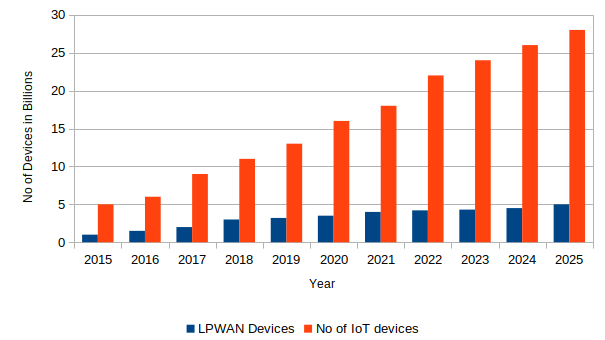
\includegraphics[width=\linewidth,height=9cm]{Images/LPWAN_growth.png}
  \centering
  \caption{Projected growth of LPWAN by Nokia \cite{nokiaresource}}
  \label{fig:Projected Growth of LPWAN}
\end{figure}
\newpage

\subsection{Motivation and Research Objectives}\label{motivation}

The promising prospects of LPWAN has encouraged the industries to adopt this technology in industrial IoT applications. \par
NB-IoT offers high; QOS, reliability, scalability, payload length but at the same time compromises with Sigfox in terms of coverage range, cost efficiency, network deployment and battery life \cite{mekki2019comparative}. Both these technologies holds a competitive market in Estonia but unfortunately, currently does not have uptake yet due to very minimum technological awareness among the application users. Application users demand strong network coverage before they are interested in developing business use cases, and LPWAN operators require consumers and enterprises demands or business cases before deploying and strengthening the current network. This leads to a paradoxical situation where both parties don't come to agreement. These situations can be jointly mitigated by strong understanding of the technology. These understandings don't come by the fact from great theoretical and simulations analysis, absence of empirical evidence largely contribute to general uncertainty of understanding the technology and results in slower adoption rate towards the technology. This thesis also focuses on advantages, disadvantages and challenges of LPWAN primarily Sigfox and NB-IoT in different deployment scenarios. By conducting bridging this gap by providing the empirical results by focusing on below research objectives. 
\renewcommand{\labelenumi}{\roman{enumi}}
\paragraph{Research Objectives}
\begin{enumerate}
    \item Evaluation of the radio frequency parameters for e.g., RSSI, RSRP, RSRQ, SINR, and packet loss among NB-IoT Vs Sigfox or licensed Vs Unlicensed frequency spectrum in different deployment scenarios are the key focus of this end point experiment.
    \item Evaluate two mobile network operator (MNO) performance in guard-band NB-IoT scheme.
    \item Behaviour of UEs in respect to co-axial interference.
\end{enumerate}
 Consequently, the above objectives defines the stability, robustness, and capabilities of both technologies which in turn will help application user in decision making.
\subsection{Thesis Structure}
The remainder of this thesis is divided into 5 chapters. Chapter \ref{technology background} describes the technology overview of LPWAN technologies - Sigfox and NB-IoT explaining them in the depth; Chapter \ref{related work} presents the previous research contributions done on this topic. Chapter \ref{Results and Methodology} describes the experimental setup followed with the results and finally, Chapter \ref{conclusion} concludes this thesis with future works.

\newpage
\section{Technology Background}\label{technology background}
\TODO{re-write this para}

\subsection{Low Power Wide Area Network (LPWAN)}
The paradigm LPWAN has emerged in recent years therefore not every IoT application matches to one specific requirement,same is the case with the IoT connectivity which does not match for all the application.LPWAN fits well to those applications which aim to have low cost of operation, long battery life , low throughput, wide area connectivity which enables devices to send tiny data over large geographical region and low power consumption so that deployed devices are operational for many years (>10 yrs). According to reports the coverage range can reach up to 5km in urban areas and up to 15km in rural areas \cite{centenaro2016long} and some even pointing to 30km range in rural areas \cite{petajajarvi2016evaluation} Figure \ref{fig:LPWAN Vs Other Wireless Technologies} compares LPWAN with other wireless technologies.

%figure3: 
\begin{figure}[H]
  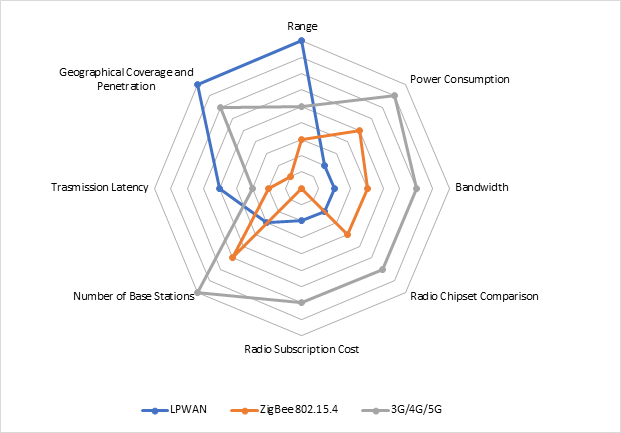
\includegraphics[trim={3cm 0 4cm 0},width=\columnwidth,height=8.5cm,keepaspectratio]{Images/lpwan_radar_2.png}
  \centering
  \caption{LPWAN Vs Other Wireless Technologies \cite{lpwanradar}}
  \label{fig:LPWAN Vs Other Wireless Technologies}
\end{figure}

The technology is broadly classified into two categories: Licensed (e.g., NB-IoT, LTE-M-IoT) and Non licensed (e.g.,Sigfox,Telensa,LoRa, RPMA, NB-Fi, Weightless) based on frequency spectrum \cite{8612009} and further Non-Licensed are sub categorised as Ultra Narrow Band (UNB) (e.g., Sigfox) and Spread Spectrum (SS) (e.g.,LoRa) based on physical layer communication \cite{8544414}. Table \ref{table:LPWAN comparison} is extracted from \cite{LPWANspecs}, illustrates the comparison of specification among various LPWAN technologies. \par

% Please add the following required packages to your document preamble:
% \usepackage[table,xcdraw]{xcolor}
% If you use beamer only pass "xcolor=table" option, i.e. \documentclass[xcolor=table]{beamer}
\begin{table}[H]
\caption{Technical specification comparison of LPWAN technologies \cite{LPWANspecs}.}
\resizebox{\textwidth}{!}{%
\begin{tabular}{|c|c|c|c|c|}
\hline

Feature                                & Sigfox UNB      & LoRa            & LTE-M              & NB-IoT               \\ \hline
\textbf{Frequency}                     & Sub-GHz ISM     & Sub-GHz ISM     & Licensed           & Licensed             \\ \hline
\textbf{Minimum Bandwidth}             & 100 Hz or 600Hz & 125 kHz         & 180 kHz            & 3.75 kHz             \\ \hline
\textbf{Effective Bandwidth}           & 300 Hz          & 3 khz           & 10 kHz             & 3 khz                \\ \hline
\textbf{Data Rate}                     & 100 bps         & 0.3-38.4 kbps   & Up to 1000kbps     & Up to 100 kbps       \\ \hline
\textbf{Modulation}                    & D-BPSK          & CSS, GFSK       & BPSK, QPSK, 16 QAM & $\pi$/2-BPSK, $\pi$/4-QPSK \\ \hline
\textbf{Media Access Control (MAC)}    & Unslotted ALOHA & Unslotted ALOHA & SC-FDMA            & SC-FDMA              \\ \hline
\textbf{Receiver Senstivity}           & -147dBM         & -137 dBm        & 23 dBm             & -137 dBm             \\ \hline
\textbf{Default Transmitted Power}     & 15 dBm          & 20 dBm          & 23 dBm             & 23 dBm               \\ \hline
\textbf{Maximum Coupling Loss}         & 162 dB          & 157 dB          & 155 dB             & 160 dB               \\ \hline
\textbf{Bi- Directional Communication} & No              & Yes             & Yes                & Yes                  \\ \hline
\textbf{Over the Air Update (OTA)}     & Yes             & Yes             & Yes                & Yes                  \\ \hline
\textbf{Roaming}                       & Yes             & Yes             & Yes                & Yes                  \\ \hline
\textbf{Standard}                      & No              & LoRaWAN         & LTE (Release 12)   & LTE (Release 13)     \\ \hline
\end{tabular}}

\label{table:LPWAN comparison}
\end{table}

% Overview of LPWAN in Estonia
\subsection{Overview of LPWAN Technologies Across Estonia} \label{Overview of LPWAN in Estonia}

There are four main public LPWAN service providers in Estonia i.e. Telia Eesti AS, Elisa Eesti AS, Connected Baltics OÜ, and Levikom Eesti OÜ; each providing a different LPWAN technology across Estonia. Telia and Elisa operate the NB-IoT technology and cover around 90\% of the whole territory of Estonia by providing service to the entire population of Estonia. This covered geography is indicated by the large shaded ellipsoid in Figure \ref{fig:Overview of coverage of NB-IoT and Sigfox in Estonia}. Connected Baltics is the exclusive Sigfox operator in Estonia and covers the major cities of Estonia: Tallinn, Tartu, Pärnu and Narva by covering around 70\% of the Estonian population \cite{connected}. The geographic coverage of Sigfox across the major cities of Estonia from the Connected Baltics is indicated by small heated circles (red, blue and green) as shown in Figure \ref{fig:Overview of coverage of NB-IoT and Sigfox in Estonia} (\cite{connected}). LEVIKOM \cite{levikom} provides LoRaWAN services but no details about their coverage in Estonia and thus we have omitted showing their coverage in Figure \ref{fig:Overview of coverage of NB-IoT and Sigfox in Estonia}. \par \begin{figure}[H]
    \centering
    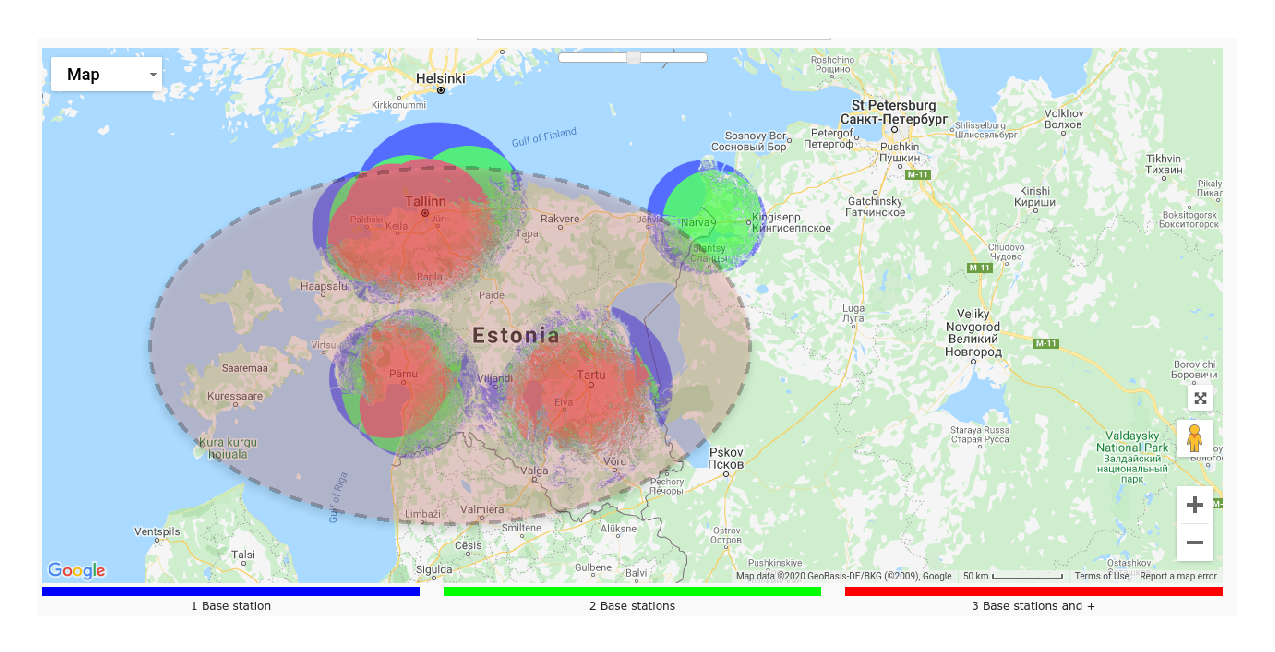
\includegraphics[width=0.9\columnwidth,height=7cm, keepaspectratio]{Images/coverage.pdf}
    \caption{Sigfox (red, blue, green smaller circles) and NB-IoT(large shaded ellipsoid) coverage in Estonia}
    \label{fig:Overview of coverage of NB-IoT and Sigfox in Estonia}
\end{figure}


%Modulation techniques in LPWAN

\subsection{Modulation Techniques in LPWAN }
In this section, we will briefly discuss the different modulations techniques and will cover the popular modulation techniques used in Sigfox and NB-IoT which is mainly focused in this thesis.
\subsubsection{Fundamentals of Modulation}
Modulation is a process of changing the characteristics of the data wave that needs to be transmitted by impressing the message signal with the high frequency.There are three main characteristics of every wave by which modulation can be achieved: frequency, amplitude and phase.Frequency in waveform refers to how many times the wave has repeated in given interval of time, Amplitude refers to the power or the strength of wave and phase refers to state of wave in particular point in time.The main objective of the modulation in telecommunication is to squeeze as much data in spectrum available. As discussed in \cite{raza2017low} LPWAN achieves long range communication by a modulating the signal with high data rate and decreasing the modulation rate in order to put more energy on each transmitted bit. The rate is measured in bits per seconds per Hz (b/s/Hz).

The two basic types of modulation used more often are:
\begin{enumerate}
    \item Analog Modulation
    \begin{itemize}
        \item Amplitude Modulation: In amplitude modulation the amplitude of the carrier wave is changed according to the signal wave. The modulating wave as a result achieves high frequency.Figure \ref{Fig:Amplitude Modulation}, signal wave that need to be transmitted is shown on top. In the middle is the carrier wave to which signal wave will be super imposed and the last one is the result.
       
% -----fig amplitude modultaion----
 \begin{figure}[H]
\begin{subfigure}[t]{\linewidth}
  \centering
  % include first image
  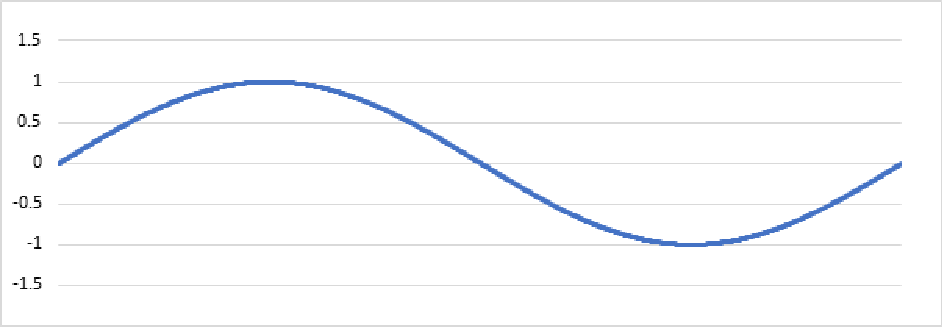
\includegraphics[width=.5\linewidth]{Images/signalWave.pdf}  
  \caption{Signal Wave}
\end{subfigure}
\begin{subfigure}[t]{\linewidth}
  \centering
  % include second image
  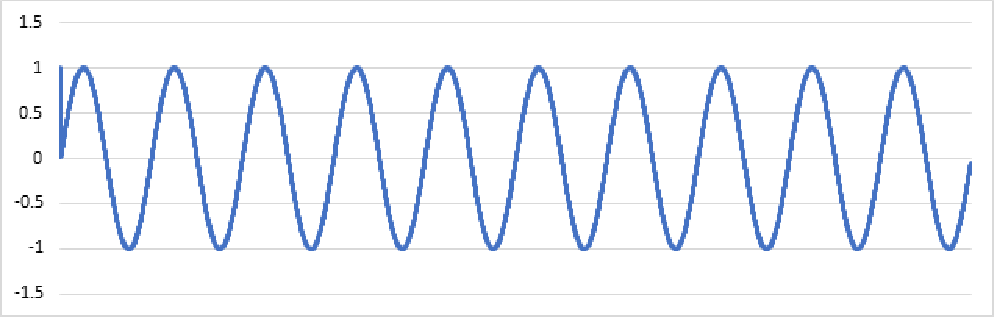
\includegraphics[width=.5\linewidth]{Images/carrierWave.pdf}  
  \caption{Carrier Wave}
  
\end{subfigure}
\begin{subfigure}[t]{\linewidth}
  \centering
  % include third image
  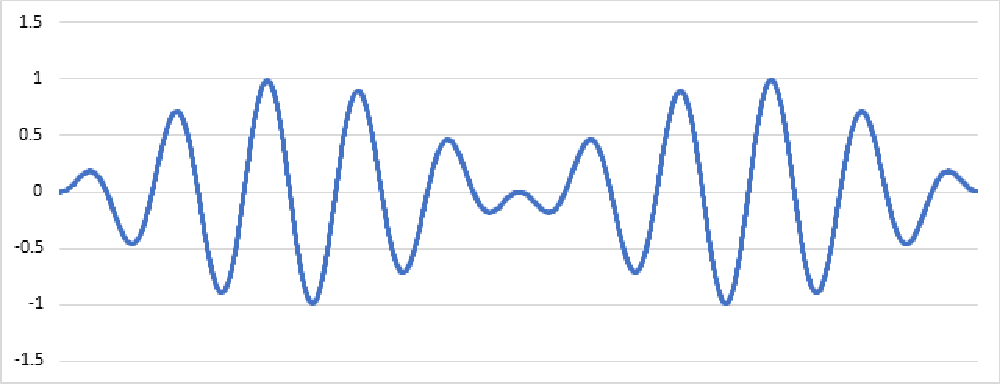
\includegraphics[width=.5\linewidth]{Images/AMwave.pdf}  
\caption{Amplitude Modulated Wave}
 \end{subfigure}
\caption{Amplitude Modulation}
 \label{Fig:Amplitude Modulation}
\end{figure}

% -----fig amplitude modultaion ends here----






        \item Frequency Modulation: In frequency modulation frequency of carrier wave is changed according to signal wave and this changed carrier wave is super imposed with the signal.The result is with signal with variable frequency. Figure \ref{fig:Frequency Modulation}, signal wave that need to be transmitted is shown on top. In the middle is the carrier wave to which signal wave will be super imposed and the last one is the result.
        
           %----figure fm modulation--- 
 \begin{figure}[H]
\begin{subfigure}[t]{\linewidth}
  \centering
  % include first image
  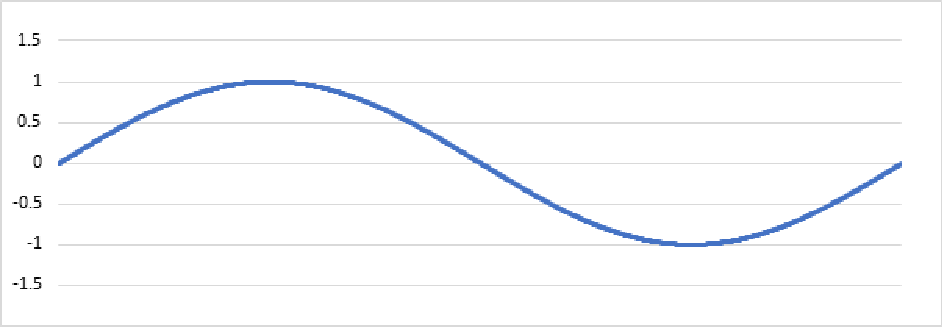
\includegraphics[width=.5\linewidth]{Images/signalWave.pdf}  
  \caption{Signal Wave}
\end{subfigure}
\begin{subfigure}[t]{\linewidth}
  \centering
  % include second image
  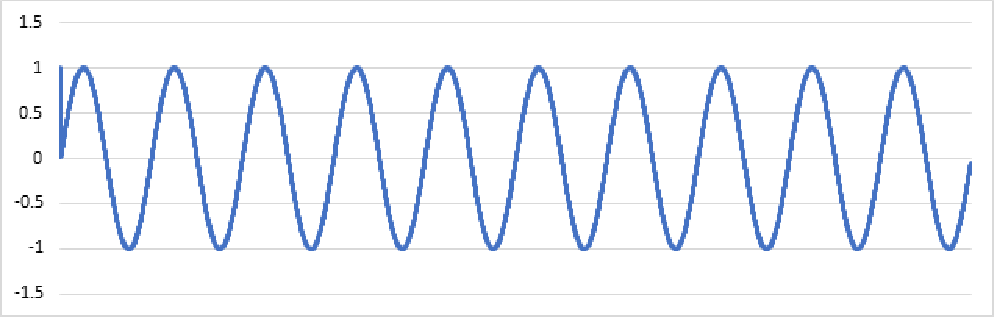
\includegraphics[width=.5\linewidth]{Images/carrierWave.pdf}  
  \caption{Carrier Wave}
  
\end{subfigure}
\begin{subfigure}[t]{\linewidth}
  \centering
  % include third image
  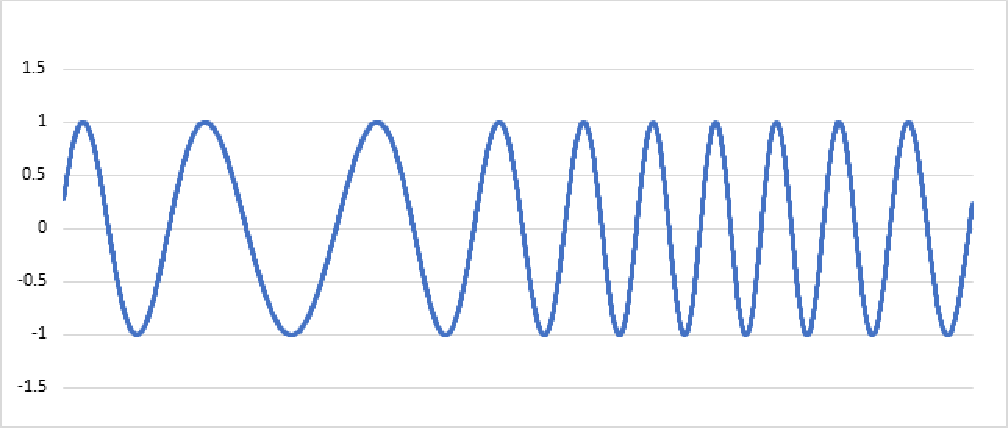
\includegraphics[width=.5\linewidth]{Images/FMwave.pdf}  
\caption{Frequency Modulated Wave}
 \end{subfigure}
\caption{Frequency Modulation}
 \label{fig:Frequency Modulation}
\end{figure}
        %----figure fm modulation ends here--- 
These above two modulation are mainly used for analog signals that are raw data and they do not represent 0's and 1's. For such digital data we use digital modulations.
    \end{itemize}
    \item Digital Modulation \newline In case of digital data change in amplitude, phase, or frequency is represented by the help of 0's and 1's and therefore it is sub-divided into to three modulations schemes i.e., amplitude shift keying (ASK), phase shift keying (FSK), and frequency shift keying (FSK). Figure \ref{fig:Digital Modulation} illustrates FSK, PSK, and ASK for the bit sequence 1010.
   
   %---fig digital modulation begins----
   \begin{figure}[H]
       \centering
       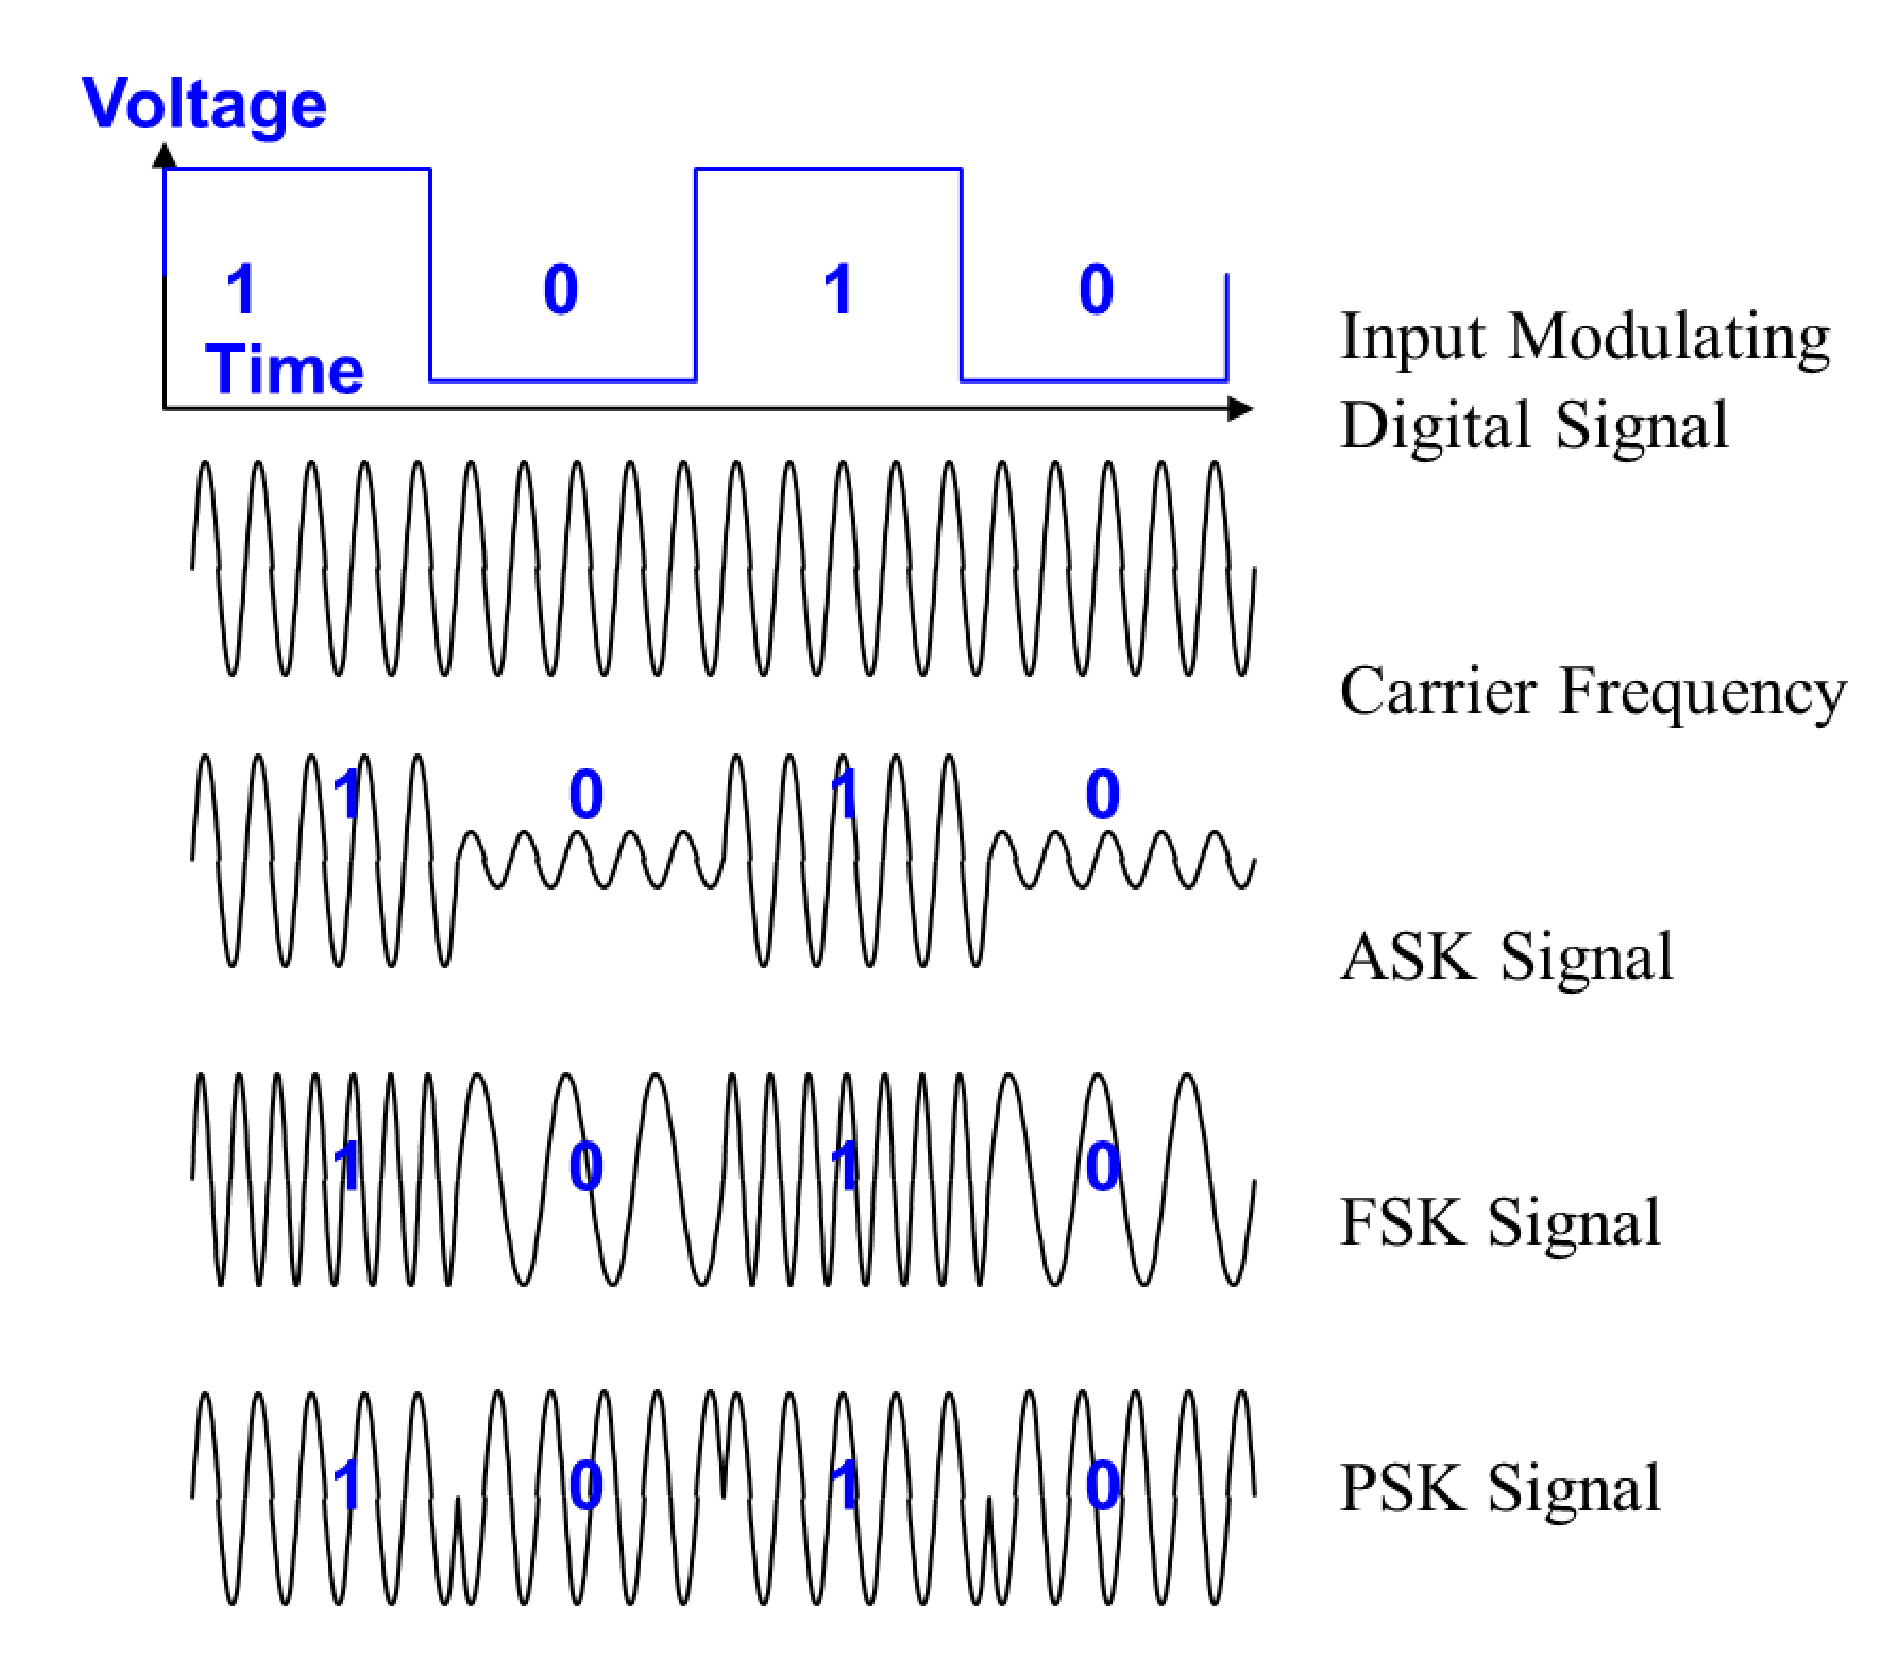
\includegraphics[width=0.5 \columnwidth]{Images/digitalModulation.pdf}
       \caption{Digital modulation}
       \label{fig:Digital Modulation}
   \end{figure}
 \end{enumerate}
 
  Sigfox uses Differential Binary Phase Shift Keying (D-BPSK) modulation in uplink and Gaussian Frequency Shift Keying (GFSK) in downlink communication. DPSK is a powerful modulation, takes only 1 Hz of the operation band to transmit 1 bit/s, this reduces the possibility of invalid translations and gives more time to demodulate, large link budget and high receiver sensitivity for the base stations; for 100 bps, sensitivity of base station is -142 dBM and at 600 bps it is -134 dBM. Furthermore, since the range of the signal weakens over distance, having only two states enhances the range and gives robustness to the signal \cite{gaddam2018comparative}.
  
  %----- fig QPSK constellation graph---
  \begin{figure}[H]
      \centering
      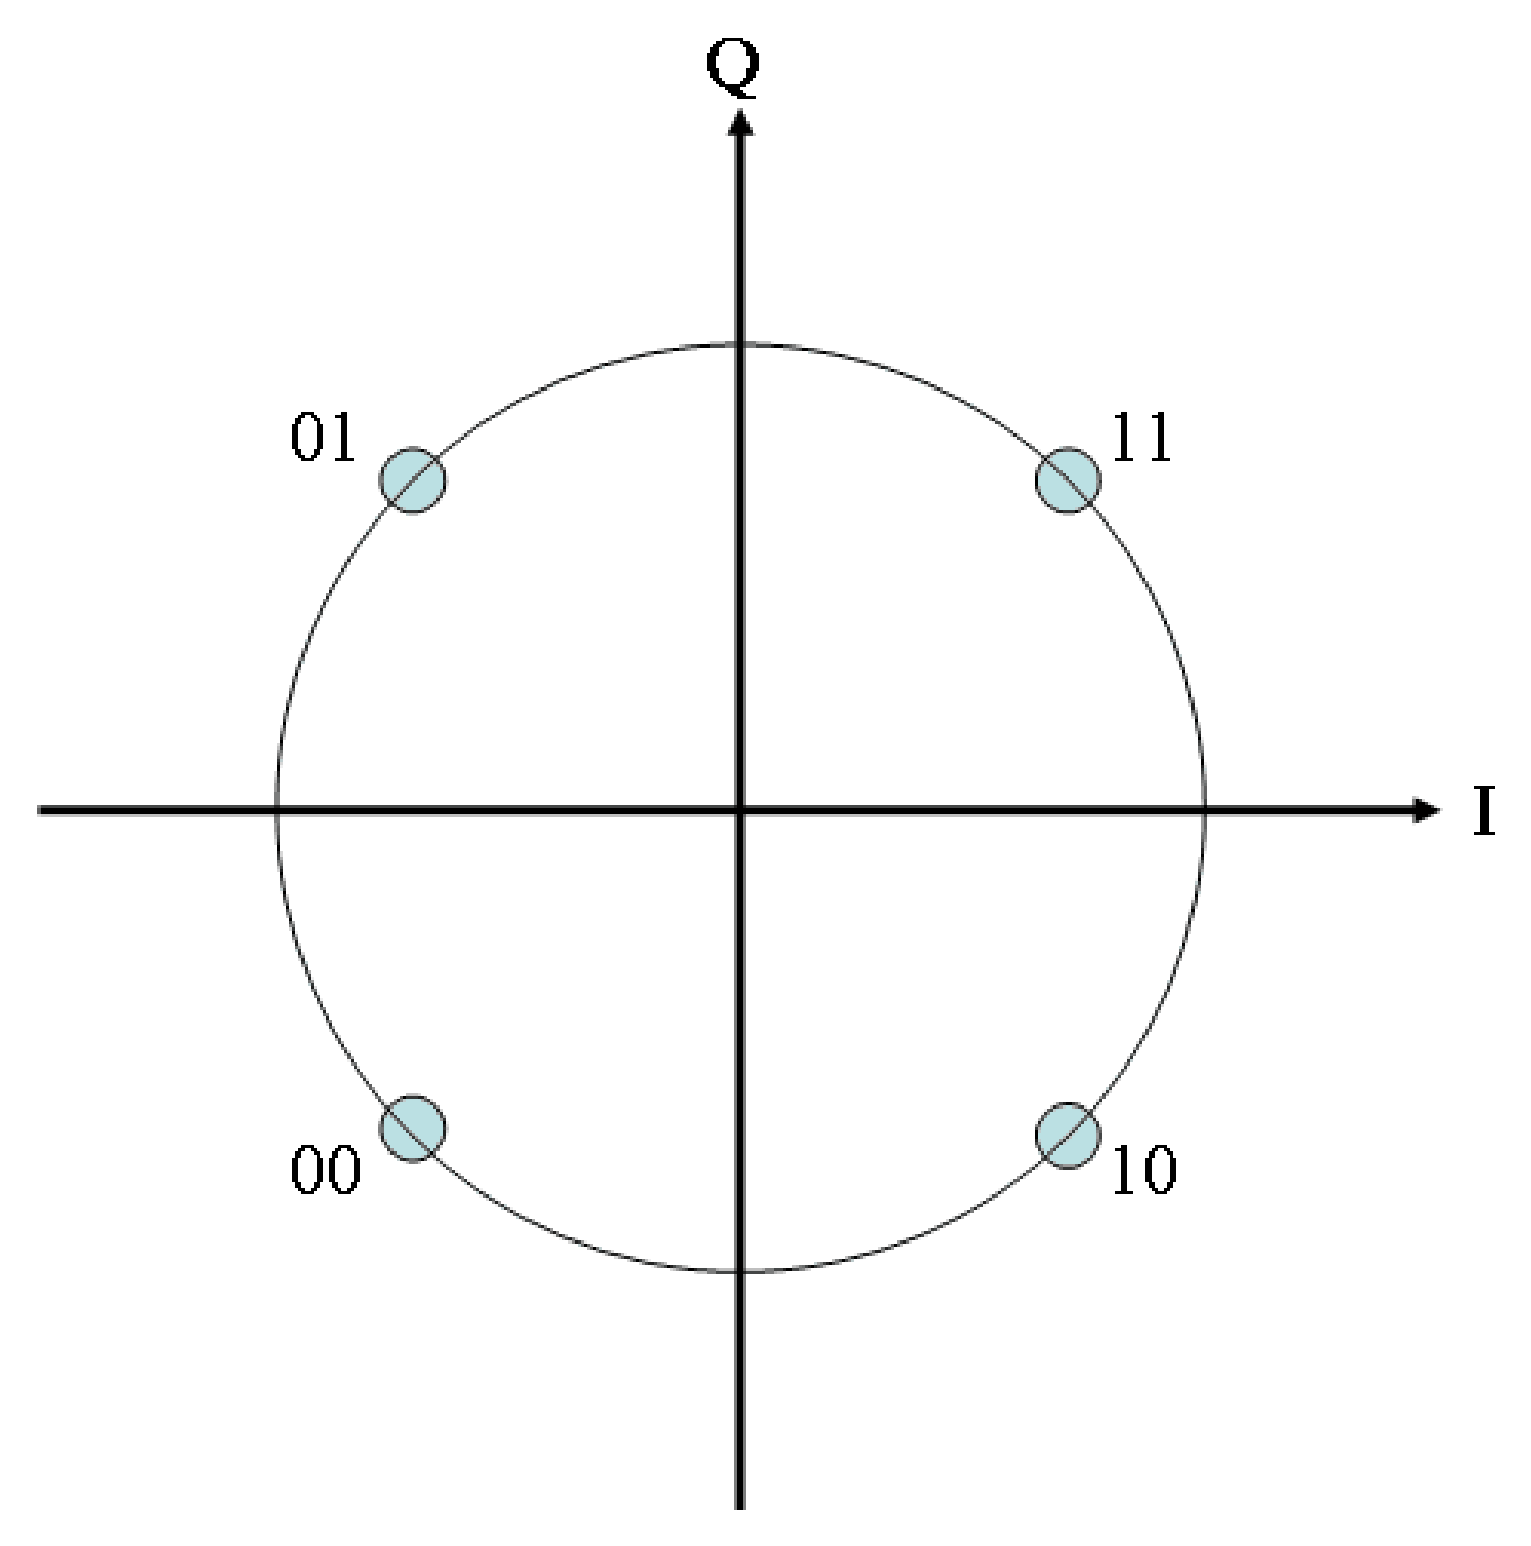
\includegraphics[width=0.5 \columnwidth, height=5cm, keepaspectratio
      ]{Images/QPSK.pdf}
      \caption{QPSK constellation graph}
      \label{fig:QPSK constellation graph}
  \end{figure}
    %----- fig QPSK constellation graph ends here ---
  NB-IoT together with other modulations scheme uses both Binary Phase Shift Keying (BPSK) and Quadrature Phase Shift Keying (QPSK) for uplink and downlink respectively. Basically in BPSK, there are two states 1 and 0, and they are often transmitted by modulating the phase of the carrier wave. Therefore, with respect to the reference  signal, a cosine wave correlates to 1, whereas sine wave correlates to 0.
  
   Furthermore, Digital modulation can also be represented in a form of constellation graph, where amplitude is distance from the origin. Figure \ref{fig:QPSK constellation graph}, represent constellation graph of Quadrature Phase Shift Keying (QPSK). The phase of the signal is denoted by angled formed with 'I' axis and it can have up to four data points 00, 01, 10 and 11.

 To summarise everything, almost all the LPWAN technologies reduces their modulation rates to maintain high energy of each transmitted bit. By doing this, the base stations are able to translate even the weakest signals without any errors.


   



\subsection{Overview of Sigfox}
\subsubsection{Introduction}
The technology was founded in 2009 in France in a city Toulouse which is also known as IoT Valley of France.At the time of writing this thesis Sigfox is spread in 70 countries \cite{SigfoxCoverage} and it is operating in collaborations with different operators in these countries.It is speculated by 2020, Sigfox will complete its WAN coverage in partnership with Eutelsat by sending constellation of nano-satellites \cite{SigfoxSatellite}.These satellite constellation will deliver connectivity across the entire globe.
Sigfox is considered to be one of the cheapest solution among all LPWAN technologies \cite{hernandez2017energy} which gives them advantage over other existing LPWAN technologies. 
\subsubsection{Technology}
As far as technology is concerned Sigfox operates in ISM and Short-Range Devices (SRD860) bands worldwide from 862 to 928 MHz.To be precise it utilizes 192kHz of SRD860 to deliver the messages using the Ultra Narrow Band Modulation.Radio configuration are divided geographically into RC zone. Table \ref{table:SigfoxRCZone} shows the radio frequencies distribution of Sigfox worldwide.

% Please add the following required packages to your document preamble:
% \usepackage[table,xcdraw]{xcolor}
% If you use beamer only pass "xcolor=table" option, i.e. \documentclass[xcolor=table]{beamer}
\begin{table}[H]
\caption{Radio Frequency distribution of Sigfox worldwide \cite{SigfoxRCZone}}
\resizebox{\textwidth}{!}{%
\begin{tabular}{|c|c|c|c|}
\hline

                         & \begin{tabular}[c]{@{}c@{}}Zone 1\\ EMEA\end{tabular} & \begin{tabular}[c]{@{}c@{}}Zone 2\\ AMERICAS/APAC 1\end{tabular} & \begin{tabular}[c]{@{}c@{}}Zone 3\\ APAC 2 (JAPAN,South Korea)\end{tabular} \\ \hline
\textbf{Frequency (MHz)} & 862-876                                                & \multicolumn{2}{c|}{902-928}                                                                                                                   \\ \hline
\textbf{RC}              & RC1                                                    & RC2,4                                                            & RC3a,RC3c,RC5                                                               \\ \hline
    \end{tabular}}

\label{table:SigfoxRCZone}
\end{table}
\newpage
\paragraph{Ultra-Narrow Band}

Ultra Narrow Band employs an ultra-narrow spectrum channel (<1KHz) to provide higher sensitivity and ultra-long distance connectivity between transmitter and receiver at the expense of maximum throughput data rates 100 bps \cite{raza2017low,bardyn2016iot,mekki2019comparative}.The demodulated spectrum is much wider than the individual transmission so that multiple devices can send message simultaneously consuming low power thus enabling the devices to have long battery life.Addition to this it offers a very good link budget due to the concentration of power in a narrow frequency band thus filtering most of the noise \cite{naik2018lpwan,7417420}, enabling the Sigfox base stations to communicate over long distances without being impacted by the noise \cite{SigfoxTechnicalDoc} Figure \ref{fig:Sigfox Technology based on UNB} depicts distribution of Sigfox in UNB.Also, UNB decreases the device's cost due to simpler and cost effective transceivers \cite{roth2018physical}.
\newline

\begin{figure}[H]
  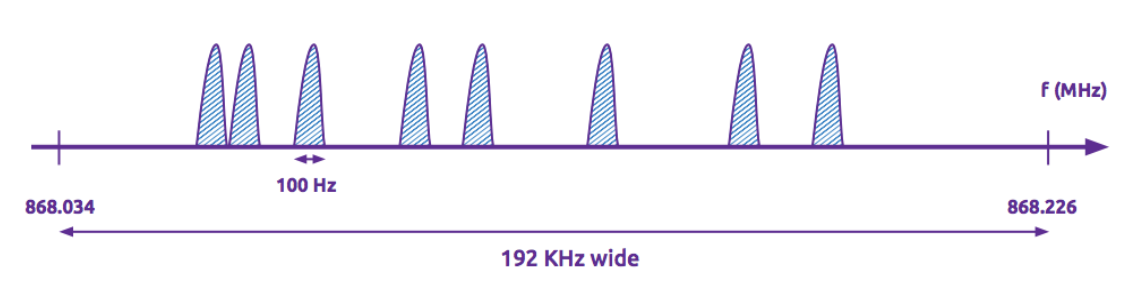
\includegraphics[width=\textwidth]{Images/sigfox_unb.png}
  \centering
  \caption{Sigfox technology based on Ultra-Narrow Band  \cite{SigfoxTechnicalDoc}.}
  \label{fig:Sigfox Technology based on UNB}
\end{figure}

Aforementioned, Sigfox is bi-directional technology there are two terminologies involved Uplink and Downlink; Uplink, refers to communications from an end device to a network server or application via one or more gateways; Downlink, refers to communications from a network server or application via one gateway to a single end device or a group of end devices \cite{farrell2018low}. Sigfox uses Differential Binary-Shift Keying (DBPSK) for uplink transmission and Gaussian Frequency-Shift Keying (GFSK) in case of downlink transmission \cite{explainingSigfox}. Downlink messages are limited in Sigfox protocol, and therefore there is a asymmetry; downlink message is sent only when device has made a downlink request in the uplink, Figure \ref{Fig:Sigfox frame structure} illustrates Sigfox uplink and downlink frame structure and Table \ref{sigfoxplan} describes the limitations and payload offerings across various subscription plans.

\begin{figure}[h]
\begin{subfigure}[t]{\columnwidth}
  \centering
  % include first image
  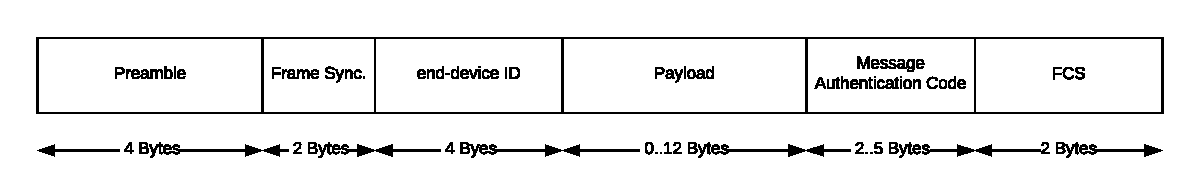
\includegraphics[width=.8\columnwidth]{Images/SigfoxUplinkFrame.pdf}  \caption{Sigfox uplink frame structure }
\end{subfigure}

\begin{subfigure}[t]{\columnwidth}
  \centering
  % include second image
  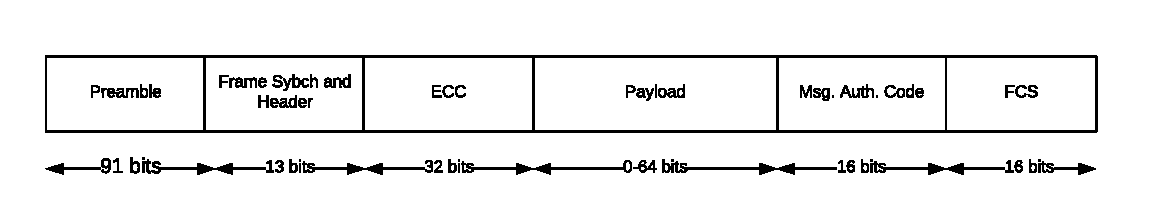
\includegraphics[width=0.8\columnwidth]{Images/SigfoxDownlinkFrame.pdf}  
  \caption{Sigfox downlink frame structure}
\end{subfigure}

\caption{Sigfox frame structure}
\label{Fig:Sigfox frame structure}
\end{figure}


\begin{table}[]
\caption{Sigfox offerings and limitations across it's subscription plans}
\centering
\resizebox{0.8\columnwidth}{!}{%
\begin{tabular}{|c|c|c|}
\hline
Plan     & Number of messages        & Max. bytes per day \\ \hline
Platinum & 140 uplinks + 4 downlinks & 1680               \\ \hline
Gold     & 100 uplinks + 2 downlinks & 1200               \\ \hline
Silver   & 50 uplinks + 1 downlink   & 600                \\ \hline
One      & 2 uplinks + no downlink   & 24                 \\ \hline
\end{tabular}%
}

\label{sigfoxplan}
\end{table}

\paragraph{Duty cycle \& Sleep Mode}
As per European Telecommunications Standards Institute (ETSI) regulations there are restrictions imposed to the technology in terms of payload transmission, according to it Sigfox can utilize 1\% of sub-band in the 868 MHz EU ISM band \cite{etsi2012electromagnetic} allowing it to send maximum 140 uplink messages and 4 downlinks consisting of 12 bytes and 8 bytes of maximum length respectively.Therefore, this roughly concludes Sigfox device may only transmit 36 seconds per hour allowing the time on air to be ~6 sec \cite{vejlgaard2017coverage}.This argument also hold valid for Sigfox that for every uplink message there cannot be downlink message as acknowledgement. Figure \ref{fig:ETSI duty Cycle and Power restriction} illustrates the duty cycle and power restriction by ETSI for various un-licensed frequencies.\\

%duty-cycle defined by ETSI
\begin{figure}[H]
  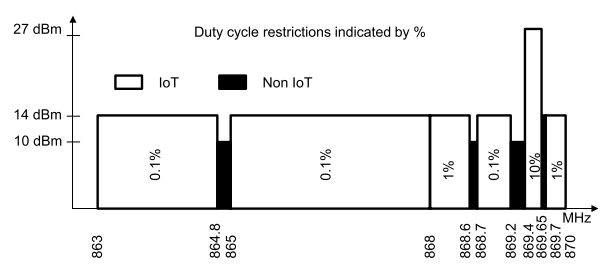
\includegraphics[width=\textwidth]{Images/duty_cycleLPWAN.png}
  \centering
  \caption{868 MHz ISM EU power and duty cycle restriction  \cite{etsi2012electromagnetic}.}
  \label{fig:ETSI duty Cycle and Power restriction}
\end{figure}

However, not able to use the channel 99\% of the time allows the device to be in deep sleep most of the time which enables them to save lot of battery and cost which in return leads to long operation (>10Yrs), Figure \ref{fig:Idle-Active states in Sigfox} .
\begin{figure}[H]
\centering
  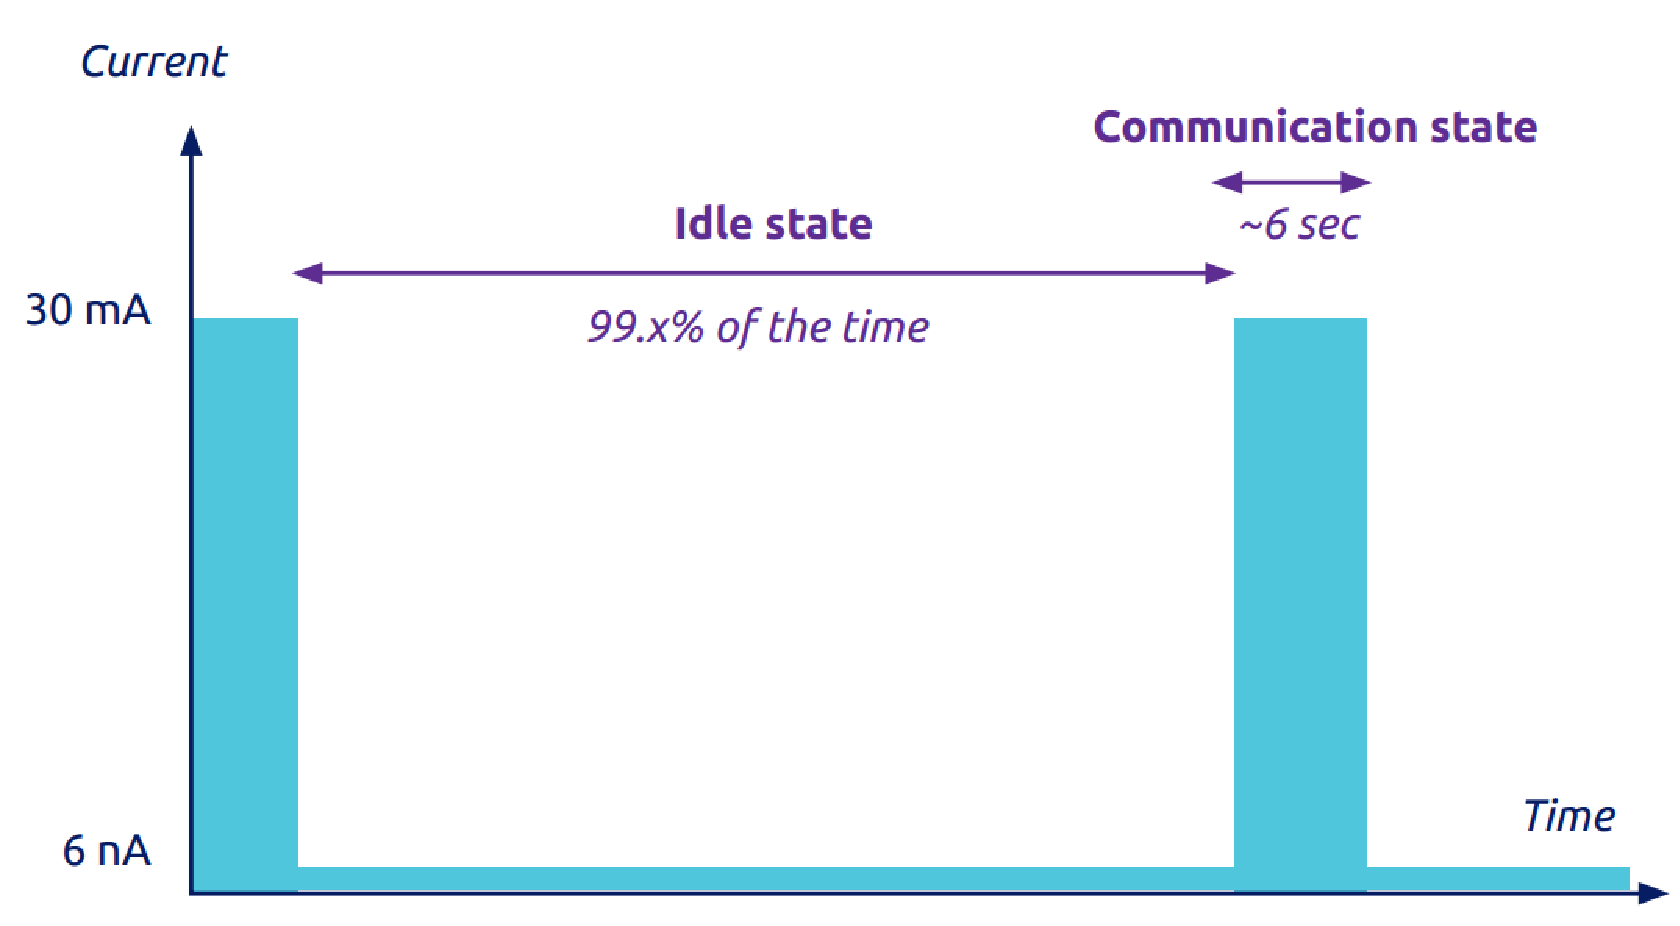
\includegraphics[width=\columnwidth, height=7cm, keepaspectratio]{Images/ActiveSleepSigfox.pdf}
  \centering
  \caption{Idle-Active states in Sigfox  \cite{SigfoxTechnicalDoc}.}
  \label{fig:Idle-Active states in Sigfox}
\end{figure}

\paragraph{Frequency and Time Diversity}
To overcome the packet loss and acknowledgement for each transmitter message Sigfox uses frequency and time diversity technique where each time the device has payload to send it transmits at three subsequent frequencies at three different slots as shown in Figure \ref{fig:Frequency and Time Diversity}.

\begin{figure}[H]
\centering
  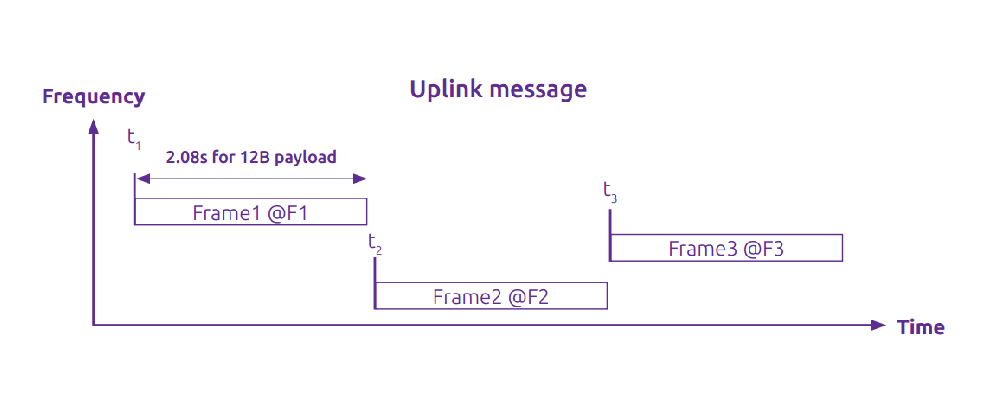
\includegraphics[width=\columnwidth]{Images/frequency_time_diversity.pdf}
  \centering
  \caption{Frequency and Time Diversity  \cite{SigfoxTechnicalDoc}}
  \label{fig:Frequency and Time Diversity}
\end{figure}

\paragraph{Spatial Diversity in Sigfox}
Spatial diversity in Sigfox defines that devices are never associated to the base stations.The emitted message is received by any near by base station and on a average the number of base station receiving the message is 3 \cite{SigfoxTechnicalDoc}. Fig \ref{fig:Spatial Diversity in Sigfox} illustrates the spatial diversity in Sigfox.

%---fig sigfox spatial diversity----
\begin{figure}[H]
  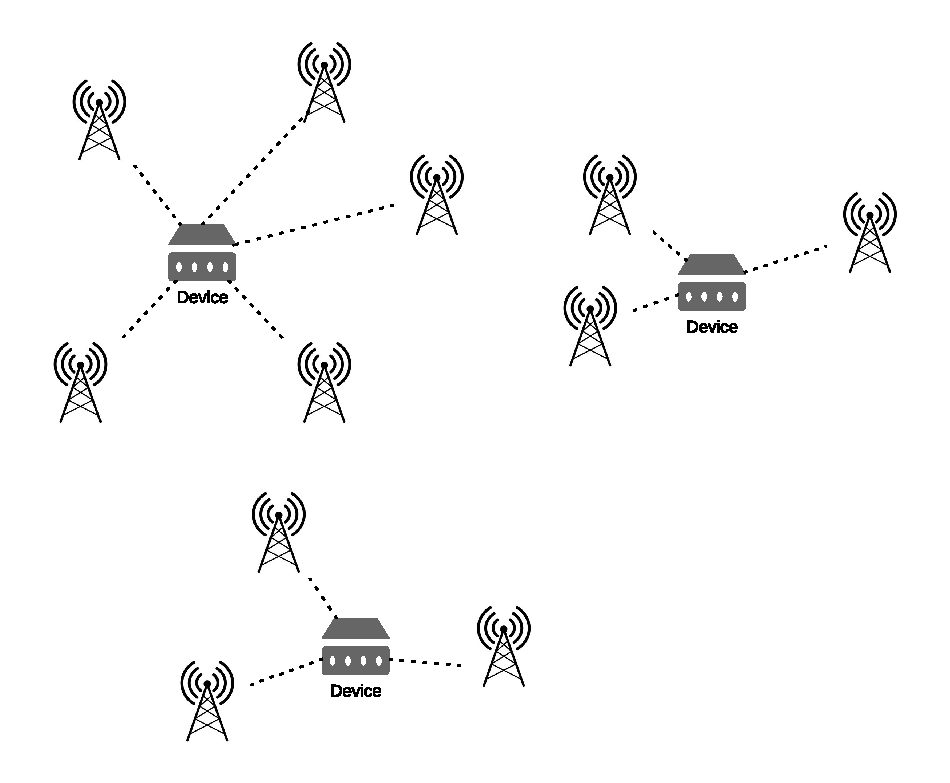
\includegraphics[width=0.5 \columnwidth, height=5cm,keepaspectratio]{Images/spatial_diversity.pdf}
  \centering
  \caption{Spatial Diversity in Sigfox, adapted from \cite{SigfoxTechnicalDoc}}
  \label{fig:Spatial Diversity in Sigfox}
\end{figure}
%---fig sigfox spatial diversity ends----


\subsubsection{Network Architecture}\label{Network Architecture}
\TODO{re-structure the sentence seq}

Sigfox architecture comprises of devices,base stations and Sigfox core network. Devices transmit their data by sending it to the nearest base stations. In this scenario, a device is not associated to the particular base station therefore at the time of communication the device transmits it's data at three different frequencies which is received by the nearest base station, upon receiving the message the base station transfers the message to the Sigfox support system which consists of the Sigfox cloud and other backend services. This approach avoids handover procedures to support device mobility.


\begin{figure}[H]
  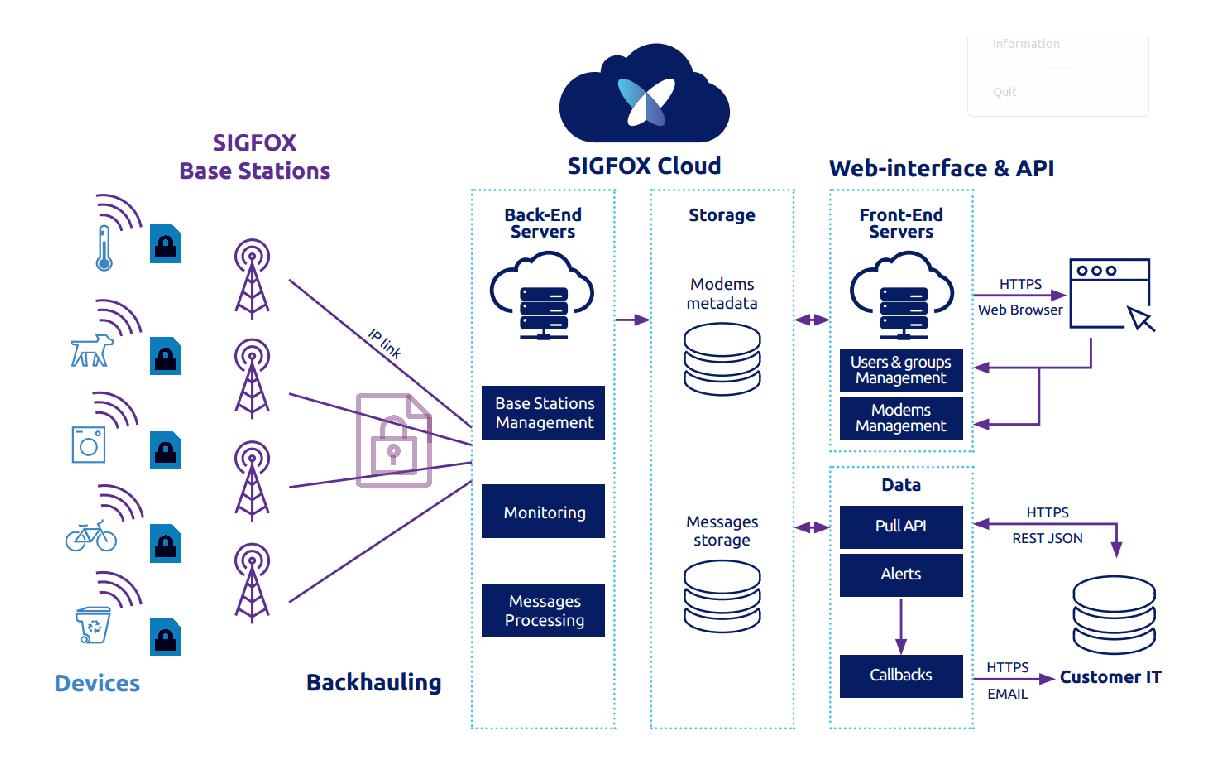
\includegraphics[width=\textwidth]{Images/sigfox_architecture.pdf}
  \centering
  \caption{Sigfox Network Architecture, adapted from \cite{SigfoxTechnicalDoc}}
  \label{fig:Sigfox Network Architecture}
\end{figure}


The back-end takes care of message processing, there can be scenario where potentially lots of replicates of the same message arrives at back-end; Sigfox cloud manages these replicas and stores one entry.The core network The core network is composed of the Service Center and the Registration Authority. The service center controls and manages the base stations and the devices. The registration authority is responsible for authorizing the network access of devices servers also monitor the status of the network and manages the base stations globally.Finally, the web interface and the API allow customers to interact and access their data with the Sigfox. As aforementioned, Sigfox does not allow acknowledgement therefore Sigfox back-end is the only platform to validate the success of message received by base station  \cite{SigfoxTechnicalDoc,gomez2019sigfox}, see Figure \ref{fig:Device's message history at Sigfox backend} which illustrates the message history of device 1B28FA5 which contains the timestamps, latency of message, data, signal quality and location of device.

\begin{figure}[h]
    \centering
    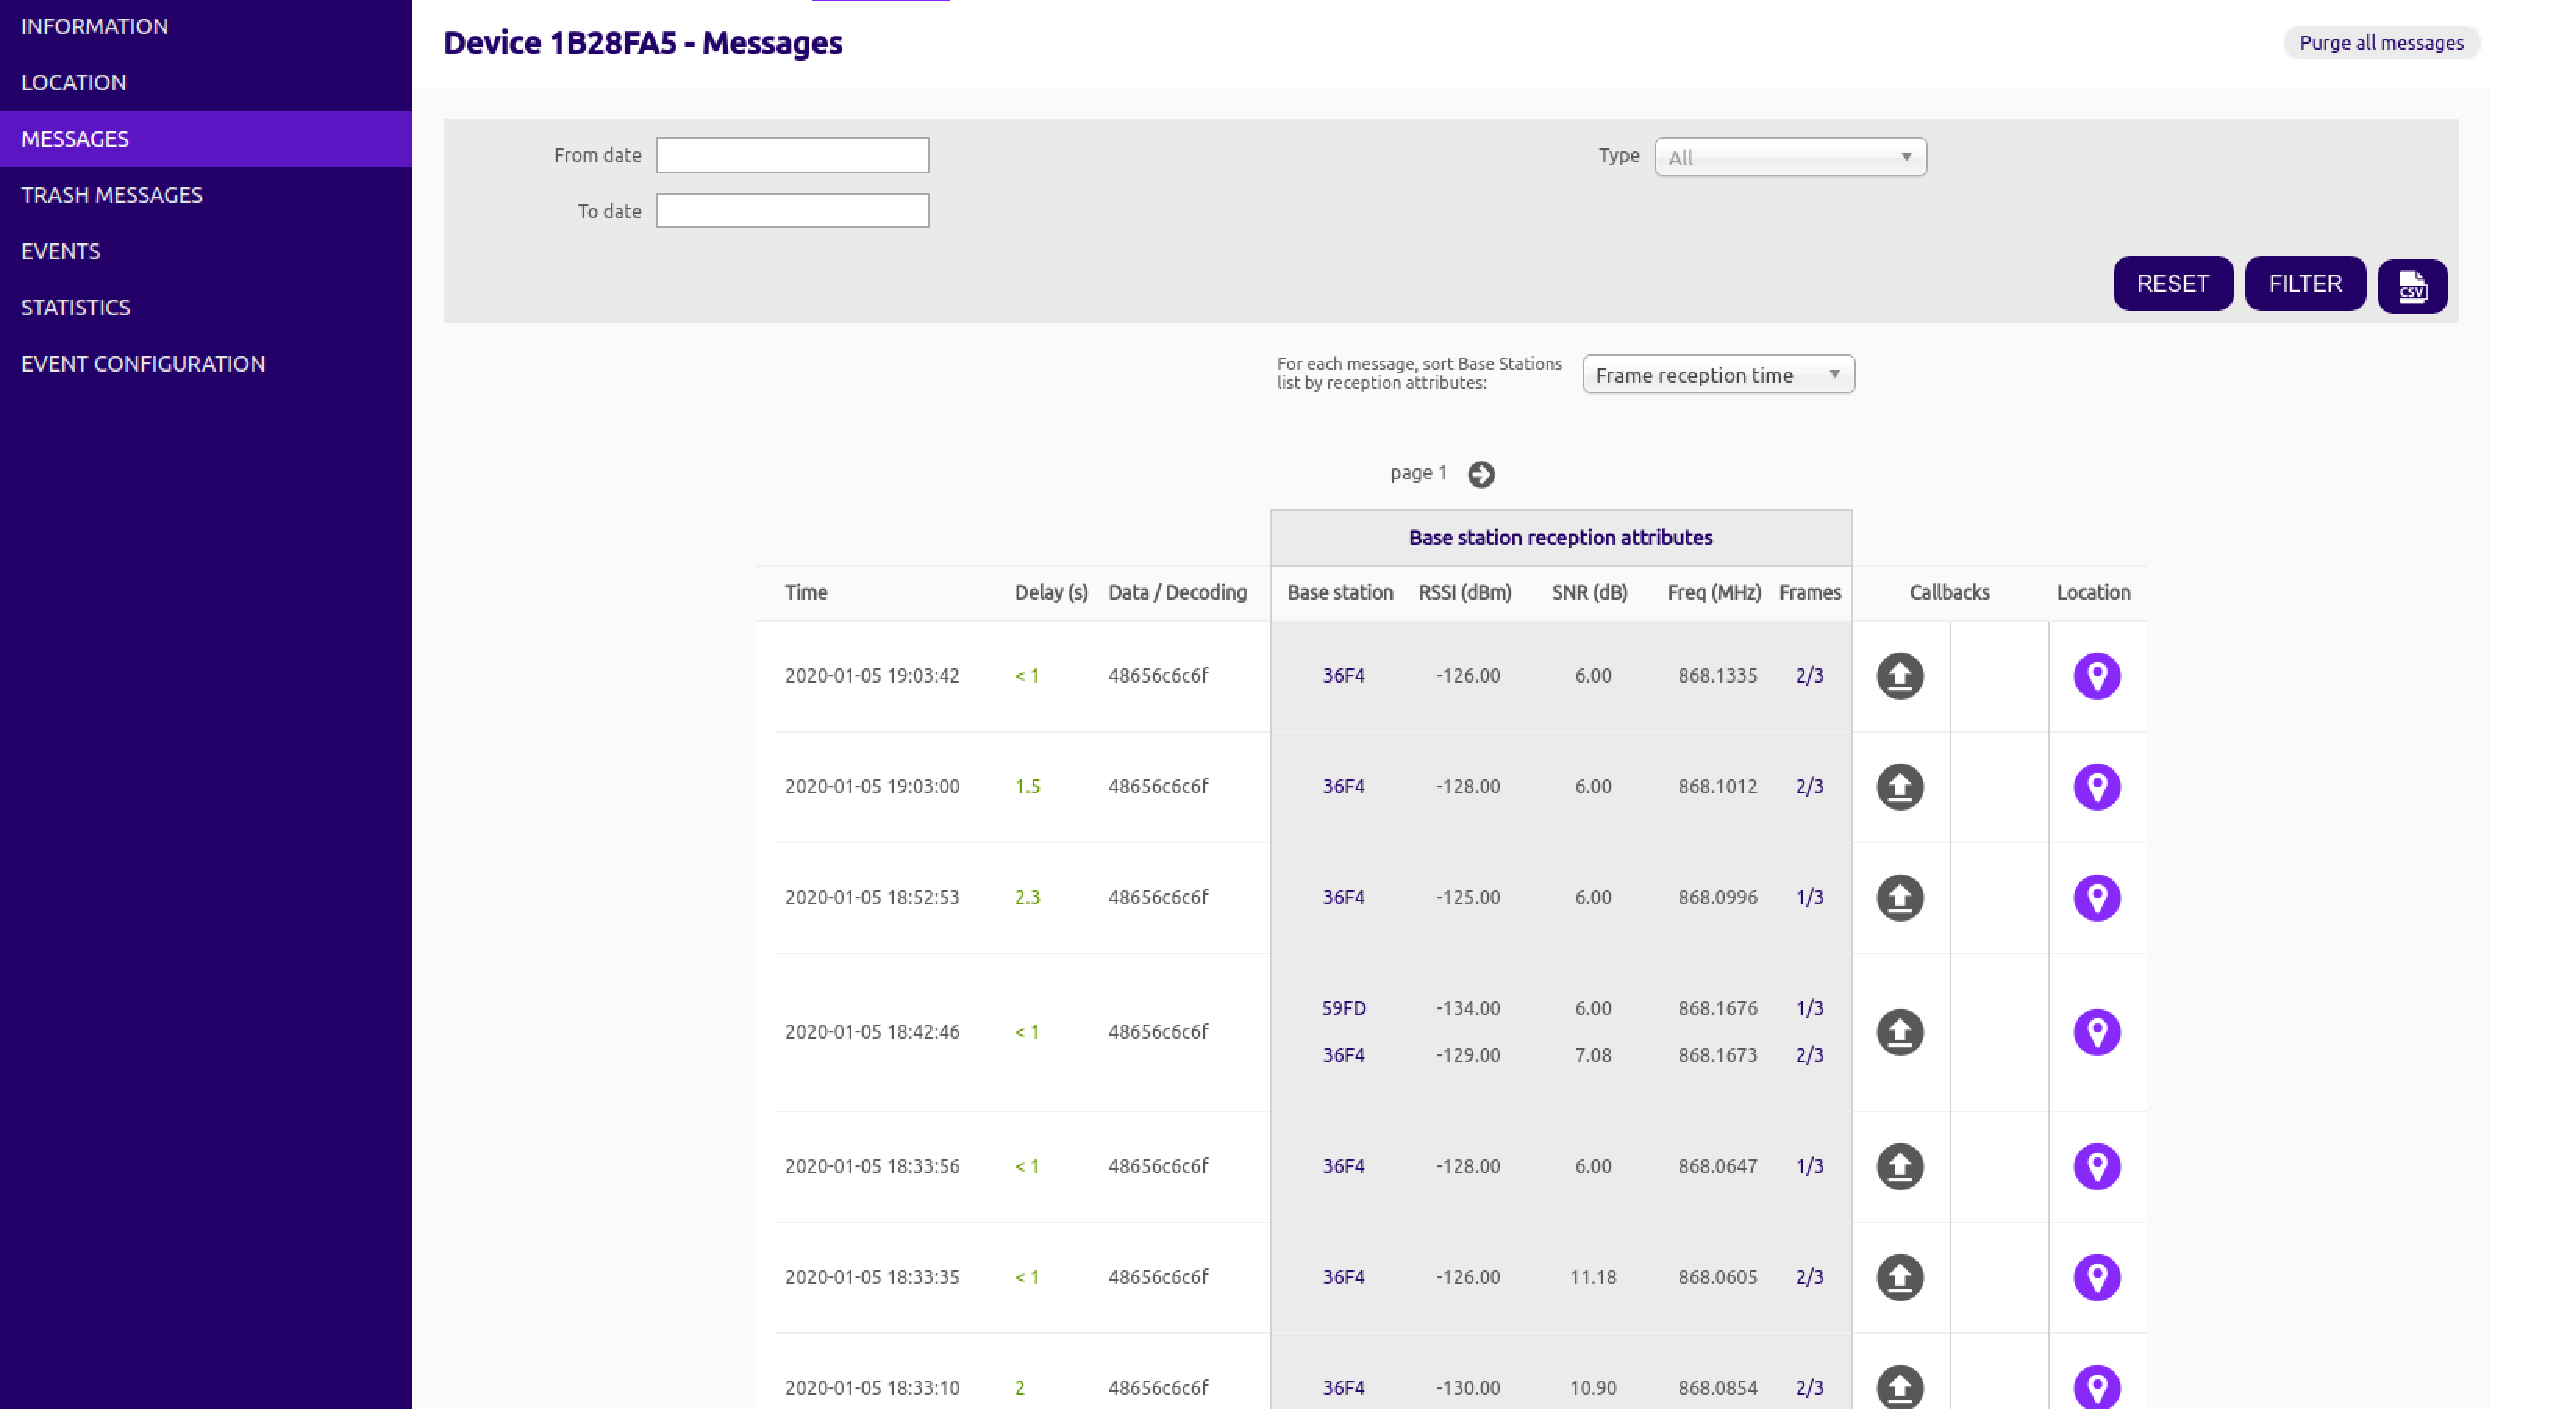
\includegraphics[width=0.8\columnwidth]{Images/sigfoxHistory.pdf}
    \caption{Message history of device at Sigfox backend}
    \label{fig:Device's message history at Sigfox backend}
\end{figure}



\subsubsection{Security}\label{Sigfox Security}
Security is one of the main challenging issue of IoT and security of one single business application is not enough. With the IoT, multiple applications
across multiple industries can share and exchange data across
different types of networks, transmitted data from the devices must have a certain security fundamentals such as integrity, confidentiality, and authentication to avoid fatal and catastrophic security attacks, and  all this should be addressed holistically.\par


%---commented Sigfox security figure, not using---
\begin{comment}
\begin{figure}[h]
    \centering
    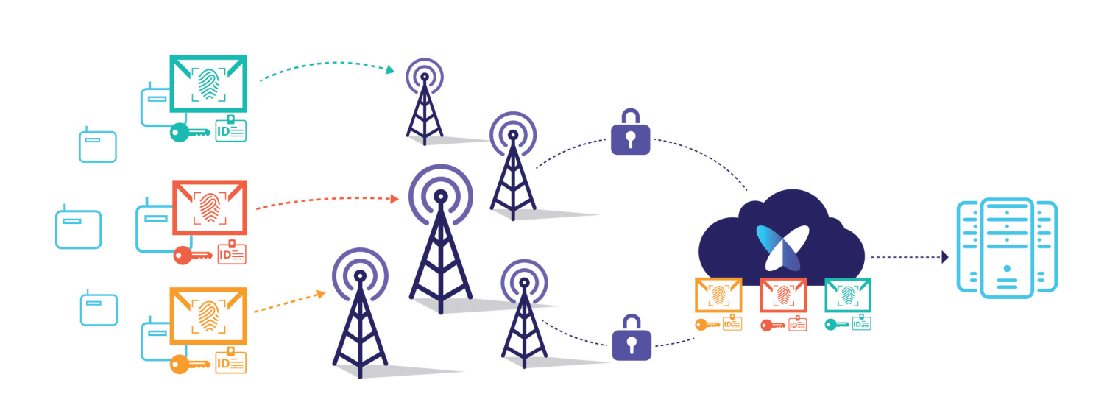
\includegraphics[width=0.9\columnwidth]{Images/sigfoxSecurity.pdf}
    \caption{Sigfox security schematics \cite{securitysigfoxwhitepaper}}
    \label{fig:Sigfox security schematics}
\end{figure}
\end{comment}
%---commented Sigfox security figure, not using---


\newpage Sigfox applies several layers of security this encompasses the complete IoT chain including devices, network infrastructure, and cloud-based services which covers the device layer to the application layer as can be seen Sigfox architecture in Figure \ref{fig:Sigfox Network Architecture}. Since, Sigfox devices are not directly connected to the internet protocol (TCP/IP); they have built-in-firewall mechanism that protects itself from denial-of-service-attacks (DDoS) and device cloning.In order to secure device's transmission and communication with the Sigfox
cloud, a Sigfox device is most of the time in sleep mode, this makes the devices immune to any possible hackers and eavesdroppers;  data is transmitted to or received from the internet which has unique authentication key, then the device broadcasts it's radio message using this unique key creating a unique signature of each message. In order to prevent duplication of message the device also adds a sequence number in the message frame. This message is picked up by several base stations and is forwarded to the Sigfox core network, which delivers it to a predefined destination, typically an IoT application. If the Sigfox device requires a response, a small limited time window is open to deliver the response to the device through the Sigfox Core Network. Thus, this design safeguards Sigfox devices, the ability to send arbitrary data entities via internet through very strict built-in-firewall.
%---end of sigfox security----------


\subsection{Overview of NB-IoT}\label{Overview of NB-IoT}

\subsubsection{Introduction}
Narrow Band IoT (NB-IoT) is a licensed LPWAN narrow band radio technology and is a extention of long-term evolution (LTE) which is designed specifically for IoT. It was developed as part of 3rd Generation Partnership Project (3GPP) project in June,2016. The journey began in May,2014 when Huawei and Vodafone proposed Narrowband Machine to Machine (NB-M2M) to 3GPP as a part of the study to cope the demands of LPWAN market; new telecom industrial players like Qualcomm also got interested, and in same year they proposed Narrowband Orthogonal Frequency Division Multiplexing (NB-OFDM) and with the result of this, in May 2015, 3GPP incorporated two proposals (i.e., NB-M2M and NB-OFDM) and formed the Narrowband Cellular IoT (NB-CIoT). In September 2015, 3GPP merged all the proposals as a work item for Release 13 which resulted in formation and recognization of NB-IoT. Since then, many telecommunication players like Ericsson, Nokia, Intel and Huwaei have been active part of standardization process \cite{5GUK,malik2018radio,mwakwata2019narrowband}.


\subsubsection{Technology}\label{NB-IoT Technology}
\paragraph{Low Channel Bandwidth}

Like LTE, NB-IoT is based on orthogonal frequency-division multiple access (OFDMA) that occupies frequency bandwidth with 180 kHz system bandwidth, which corresponds to one physical resource block (PRB) in LTE transmission. With 180 kHz of minimum spectrum requirement, NB-IoT can be deployed in three possible operational modes,i.e, i) as standalone, ii) in the guard carriers of existing LTE/UMTS spectrum, iii) within an existing LTE carrier (inband) by replacing one or more PRBs, see Figure \ref{fig:NB-IoT operational modes}. In order to support such flexible deployment scenarios, NB-IoT reuses the LTE design extensively, such as OFDM in downlink and single carrier frequency-division multiple access (SC-FDMA) in uplink \cite{8612009,malik2018radio,sinha2017survey,boisguene2017survey}. All three operational modes are only deployed  in licensed frequency bands. The maximum transmission power is either 20 or 23 dBm for uplink transmissions, while for downlink transmission, the base station may have higher transmission power, up to 46 dBm depending on the deployment \cite{farrell2018low}.\par
\begin{figure}[H]
    \centering
    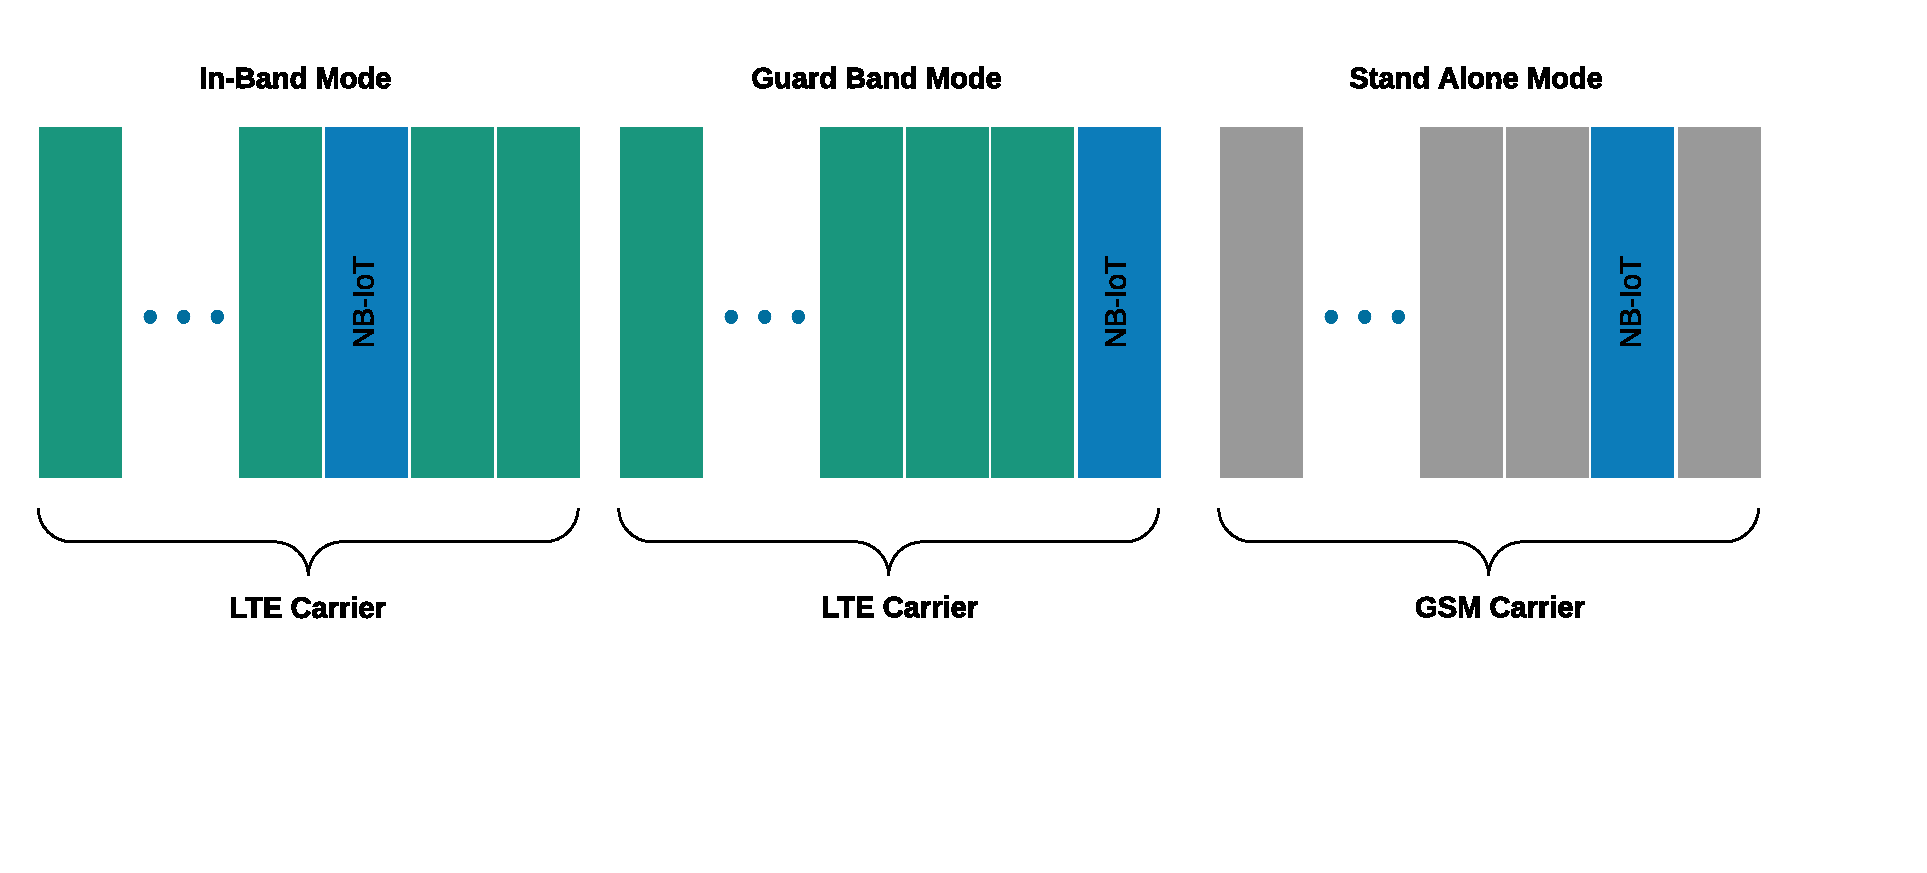
\includegraphics[width=0.9\columnwidth, height=5cm, keepaspectratio]{Images/nbiotModes.pdf}
    \caption{NB-IoT operational modes, adapted from \cite{xu2017narrowband}}
    \label{fig:NB-IoT operational modes}
\end{figure}
%---end of the NB-IoT operational mode----
The three operational modes are briefly explained below:
\renewcommand{\labelenumi}{\roman{enumi}}
\begin{enumerate}
    \item In-Band Operation Mode\newline
    In-band deployment means that the narrowband is deployed inside the LTE band and radio resources are flexibly shared between NB-IoT and normal LTE carrier \cite{farrell2018low}.
    \item  Guard Band Operation Mode\newline
    In Guard- band deployment, the narrowband uses the unused resource blocks between two adjacent LTE carriers \cite{farrell2018low}.
    \item Stand Alone Operation Mode\newline
    Standalone deployment is also supported, where the narrowband can be located alone in dedicated spectrum, which makes it possible, for example, to reframe a GSM carrier at 850/900 MHz for NB-IoT \cite{farrell2018low}.
\end{enumerate}

\paragraph{Resource grid of NB-IoT}
NB-IoT only uses 180 kHz bandwidth for both uplink and downlink, and two different carrier spacing in uplink i.e., 3.75 kHz, and 15kHz,for downlink it has only 15 kHz. In order to serve many devices it supports two schemes 1) optional multi-tone transmission and 2) mandatory single-tone transmission \cite{xu2017narrowband,malik2018radio}.Uplink, can be either single-tone or multi-tone. The 3.75kHz spacing is single-tone, and 15 kHz frequency can be utilized for both single and multi-tone.The detailed frame structure of both downlink and uplink with control channels from TR45.820 \cite{TR45.820,malik2018radio}, are as follows:

\subparagraph{Downlink Transmission:}
The frame structure of NB-IoT downlink is similar to conventional LTE, in the short time frequency of 10ms, each frame holds 10 sub-frames of 1 ms length and each sub-frame holds two slots with the length of seven OFDMs. In frequency domain it holds one PDR with 12 sub-carriers each having 15 kHz of spacing and normal cyclic prefix (CP). One symbol x of sub-carrier equals to one resource element (RE), the smallest transmission unit. RE in general is equivalent to one modulation symbol of sub-carrier i.e., 2 bits of QPSK, 4 bits of 16-QAM , and 6 bits of 64-QAM. Additionally, unlike LTE, the NB-IoT downlink physical channels and signals are primarily multiplexed in time \cite{malik2018radio}. These two physical signals and three physical channels are discussed below that are taken from  \cite{malik2018radio,ratasuk2016overview}:
%---- downlink Frame Structure----

\begin{figure}[!h]
    \centering
    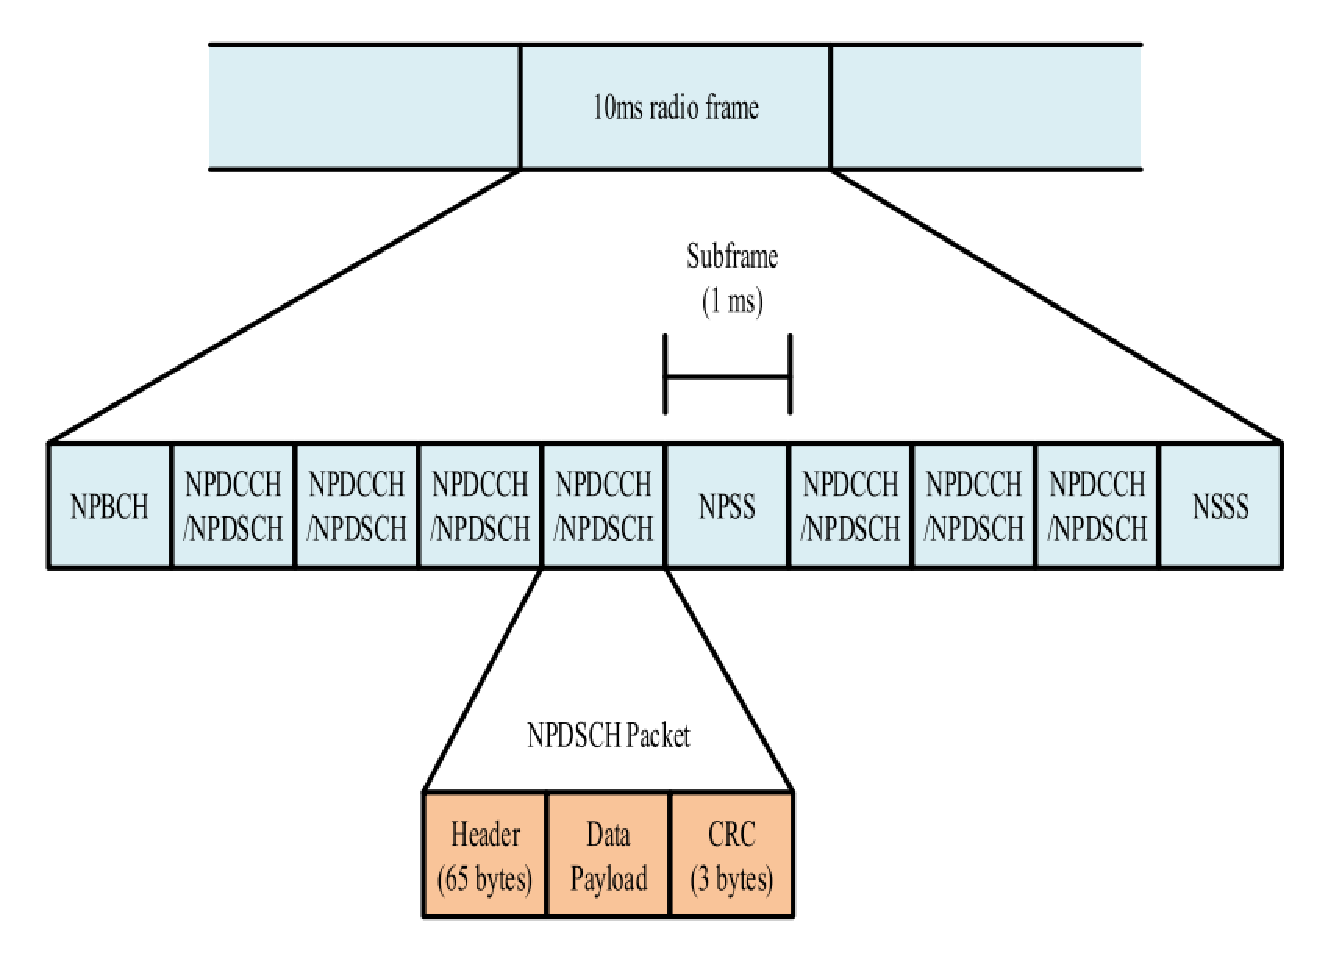
\includegraphics[width=0.9\columnwidth]{Images/nbiotDownlinkFrame.pdf}
    \caption{NB-IoT downlink frame structure \cite{malik2018radio}}
    \label{fig:NB-IoT downlink frame structure}
\end{figure}
\renewcommand{\labelenumi}{\roman{enumi}}
\begin{enumerate}

    \item \textbf {Narrowband reference signal (NRS):}
    It is used to provide phase reference at the time of demodulation of downlink channel. NRS is transmitted in all sub-frames that might be used to broadcast or downlink transmission using eight REs per antenna port.In case of in-band operation, LTE's reference signals (CRS) are also transmitted with the NB-IoT band, which is not the case in standalone and guard band operations.

    \item \textbf{ Narrowband primary and secondary synchronization signals (NPSS and NSSS):}
    NPSS transmits 5 sub-frames every 10 ms, whereas NSSS transmits 9 sub-frames periodically; these signals are used for cell search using time and frequency synchronization and cell identity detection.
    
    \item \textbf{Narrowband physical broadcast channel (NPBCH):} It stores the master information block (MIB) and it is transmitted in every sub-frame 0. In whole duration of transmission MIB is remains constant for 640 ms transmission time interval (TTI).
    
    \item \textbf{Narrowband physical downlink control channel (NPDCCH):} It is considered to be the core element of the downlink as it holds control informations like paging, random access channel (RACH) response, type of modulation being used for transmission, power control, and so on. Addition to this, it controls the data transmission between the device and the base stations (BS). The size of the control information is 23 bits which is fixed in all scenarios.
    
    \item \textbf{Narrowband physical downlink shared channel (NPDSCH)} It is considered to be main data bearing channel; holds user unicast data, some control information and the system information block (SIB). If SIB occupies the frame, it usually occupies the subframe 4 in the 16 continuous frames \cite{malik2018radio}.
 \end{enumerate}

 \subparagraph{Uplink Transmission:} As aforementioned, in NB-IoT, uplink supports both single-tone and multi-tone transmission. Multi-tone uses 15 KHz sub carrier spacing with SC-FDMA scheme and total 180 KHz bandwidth with 0.5 ns slot and 1ms sub-frame similar to LTE. However, single-tone uses both 15 kHz and 3.75 kHz sub-carrier spacing and is four times longer compared to 15 kHz with slot length of 2 ms. Each 2 ms slot contains 7 OFDM symbols with 48 sub carriers. Addition to this, in NB-IoT there is resource mapping unit (RU) which is combination of total sub-carriers (frequency domain) and number of slots (time domain). In uplink, we have two physical channels, as illustrated in Figure \ref{fig:NB-IoT uplink frame structure}.
 
 \begin{figure}[!h]
     \centering
     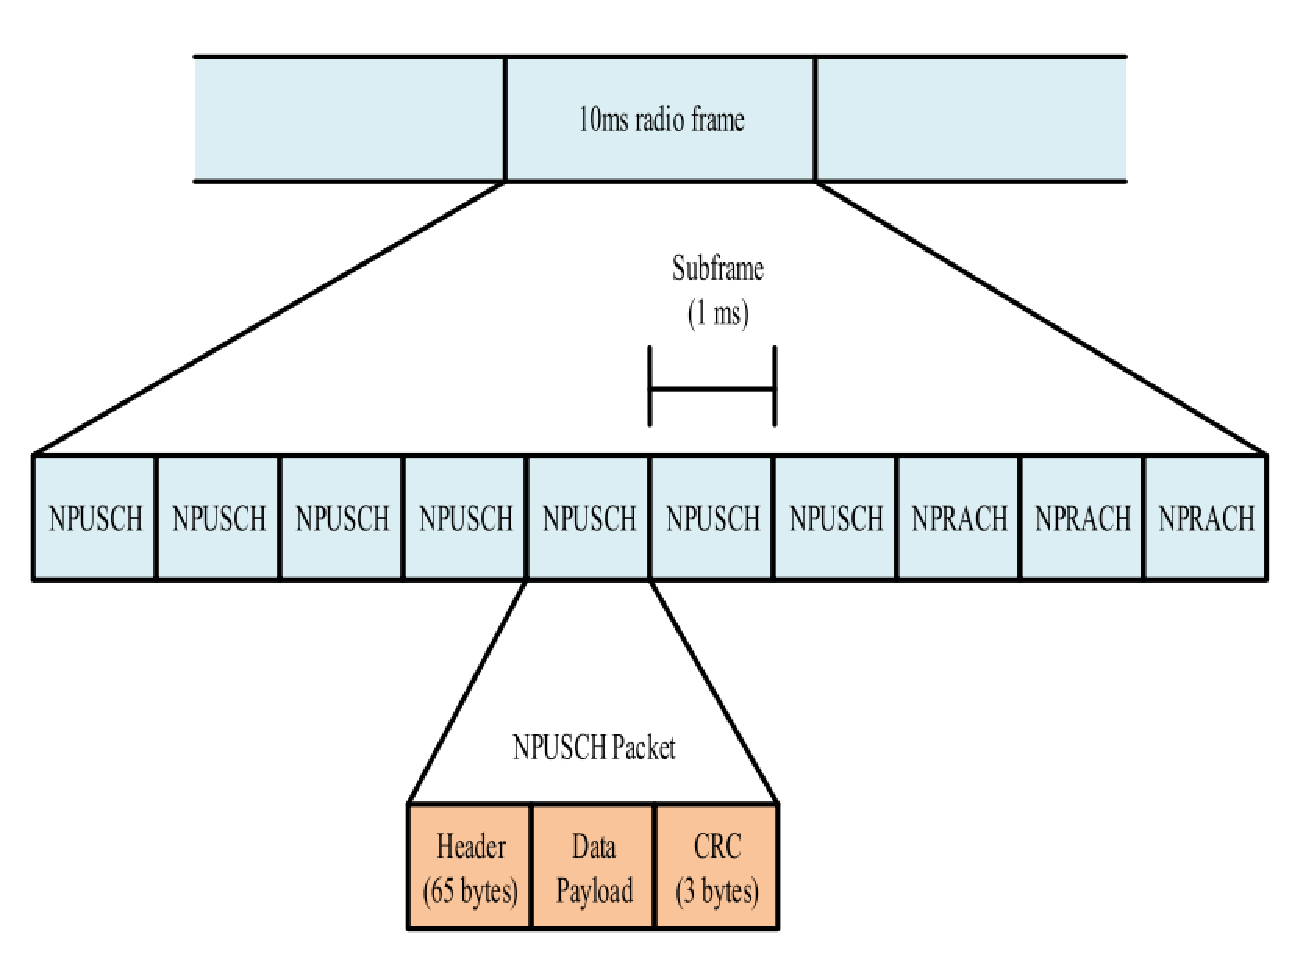
\includegraphics[width=0.9\columnwidth]{Images/nbiotUplinkFrame.pdf}
     \caption{NB-IoT uplink frame structure \cite{malik2018radio}}
     \label{fig:NB-IoT uplink frame structure}
 \end{figure}
 
 \begin{enumerate}
     \item \textbf{Demodulation Reference Signal (DMRS):} DMRS is multiplexed with uplink data therefore it is only transmitted in RUs.
     \item \textbf{Narrow Physical Random Access Channel (NPRACH):} It helps devices to connect to the base stations.The base stations estimates the uplink timings by taking help of random access preamble which is sent by user terminal, it is necessary to issue a timing advance command just to maintain uplink orthogonality among various users.  
     \item \textbf{Narrow Uplink Shared Channel (NPUSCH):} 
     
      Unlike LTE, both the data and control information are carried over the uplink shared channel in 10 RU block size. This channel co-exist with two formats; Format 1, is used for carrying uplink data and uses turbo code for error correction. Format 2, is used for hybrid automatic repeat request (HARQ) acknowledgment for downlink data with maximum 128 repetitions \cite{malik2018radio}.
    
 \end{enumerate}
 
\paragraph{Power saving mechanism}
In order to extend the battery life of NB-IoT devices up to 10 years, 3GPP adopts two features Power Saving Mode (PSM) and Extended Discontinuous Reception (eDRx) , see Figure \ref{fig:Power saving in NB-IoT}.\par

eDRX, is a mechanism that enables device to turn-off part of it's circuitry to save power \cite{el2018evaluating}; the eDRX cycle can last up to 3 hours \cite{farrell2018low} and during this cycle the device can listen to the downlink control channel for downlink messages, also known as by term  $Narrowband\  Physical\  Downlink\  Channel\  (NPD-CCH)$. This listening process is referred as paging \cite{sultania2019implementation}.\par 

\begin{figure}[H]
    \centering
    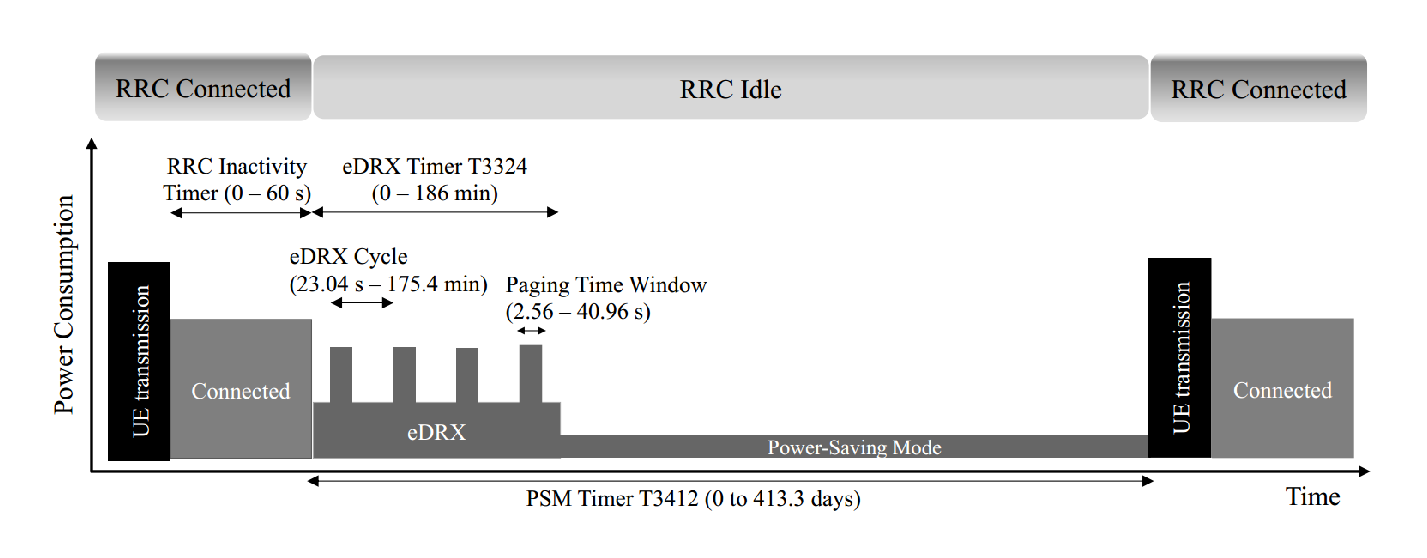
\includegraphics[width=0.9\columnwidth]{Images/nbiotDRXcycle.pdf}
    \caption{Power saving in NB-IoT \cite{sultania2019implementation} }
    \label{fig:Power saving in NB-IoT}
\end{figure}

PSM, is a mechanism which enables the device to go in a deep sleep state by turning-off it's radio up to maximum 413 days \cite{sultania2019implementation}; and wakes up only for uplink transmission. In order to update the network about it's availability, the device performs periodic tracking area up- dates (TAU) after a configurable TAU timer has expires. The device then remains reachable and connected for paging during the paging time window (PTW) which is configurable. Once the PTW expires, it again enters into  deep sleep mode (PSM mode) and becomes dormant and unreachable until the next periodic TAU occurs. During PSM mode, the device switches off its circuitry yet is still registered to the network. The advantage of such an approach lies in the fact that the device can wake up immediately from PSM mode without having to re-establish the network and PDN connections. This prevents extra power consumption due to additional signaling messages transmission. PSM feature also maximizes the downtime of the device, which significantly reduces battery consumption \cite{rohdepowernbiot}.\par
%--end _-------

\paragraph{Coverage Enhancement}
As per 3GPP release 13, NB-IoT offers 164dB coverage with a potential to add 50k devices per cell and also has ability to scale up by just adding more NB-IoT carriers \cite{raza2017low,farrell2018low}, which gives ten times coverage enhancement to indoor and deep indoor scenarios compared to GPRS. In order to achieve +20dB coverage extension, repetition is the main solution in given bandwidth. NB-IoT offers maximum 128 repetition considering 21dB gain in theoretical \cite{bao2018coverage,mwakwata2019narrowband}. In the study done in Tallinn University of Technology by author \cite{malik2019nb}; a total of 20 nodes were deployed in different locations and scenarios, study concluded with the claim of +20 dB extension with a areal coverage of 700m in urban scenario. However in \cite{mekki2019comparative}, author claims that NB-IoT is not suitable technology when it comes to rural deployment due to it's lowest range and coverage capabilities (i.e., range <10 km).

\subsubsection{Network Architecture}

A basic architecture of NB-IoT is shown in Figure \ref{fig:NB-IoT Architecture} and NB-IoT is divided into three main parts:


\renewcommand{\labelenumi}{\roman{enumi}}
\begin{enumerate}

    \item End Devices: These devices benefit the IoT application by sending the valuable data to the customer platforms.They all are connected through the proper NB-IoT network using narrow band sim-cards from telecom operators.
    \item Base stations: These base stations are usually owned and managed by local telecom operators and base stations are often referred as eNodeB or eNB.
    \item NB-IoT core network: It provides the interface between the NB-IoT base stations and NB-IoT cloud. NB-IoT uses the same network architecture as conventional LTE network; similar to LTE, NB-IoT core network depends on the evolved-packet-system (EPS) and two optimizations for cellular IoT (CIoT).
\end{enumerate}
%--fig nb-iot acrhitecture---
\begin{figure}[H]
    \centering
    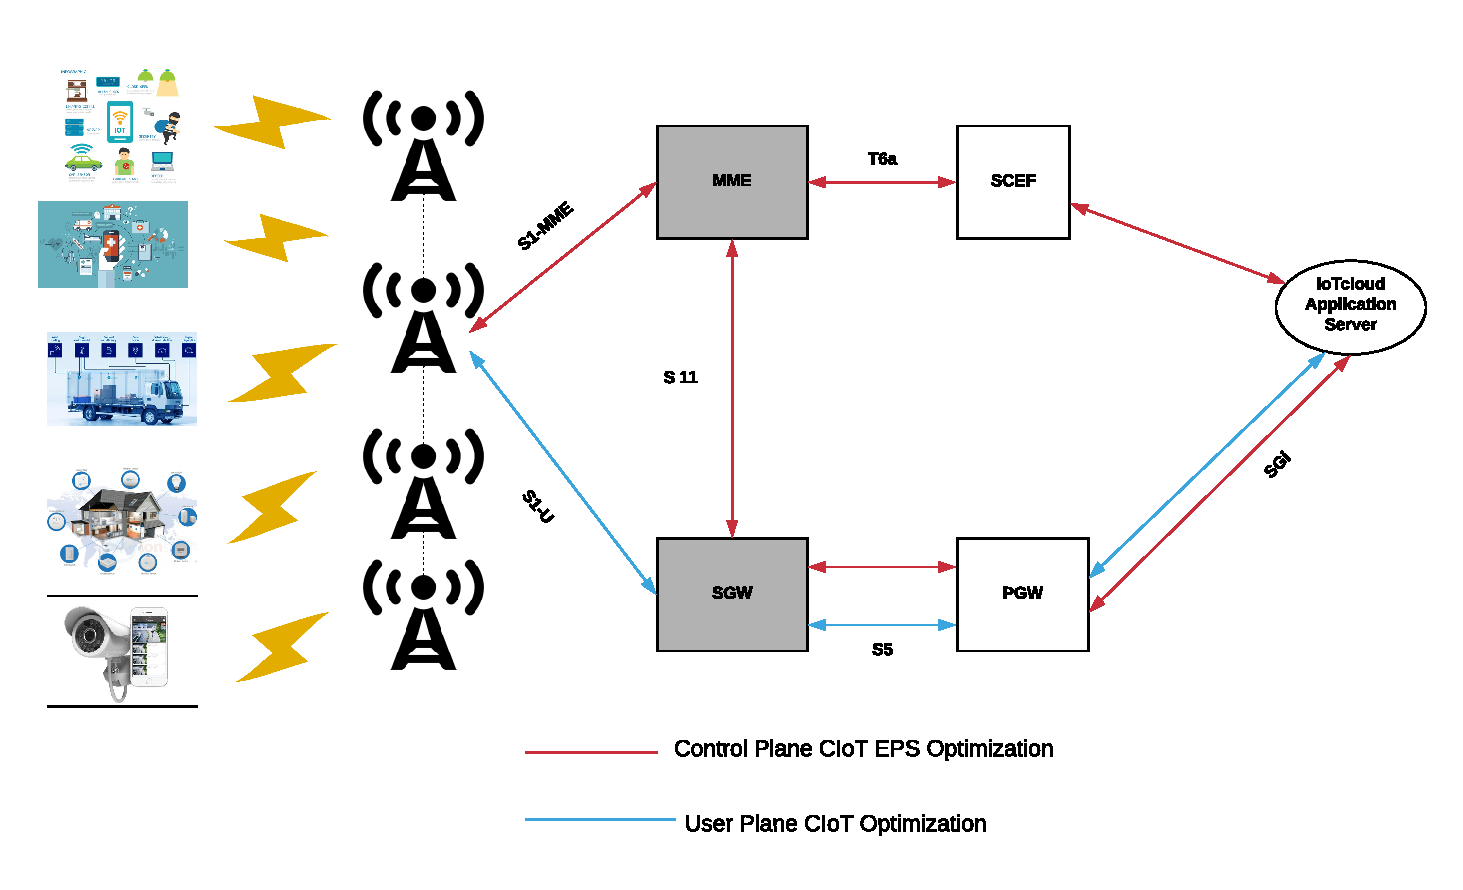
\includegraphics[width=\columnwidth, height=7cm, keepaspectratio]{Images/nb-iotArchitecture.pdf}
    \caption{Architecture of NB-IoT, adapted from \cite{jaber2019study}}
    \label{fig:NB-IoT Architecture}
\end{figure}
%--fig nb-iot acrhitecture---
\paragraph{$Control \ plane\ CIoT\ optimization$}

This optimization adopts the control plane to transmit device's data packets. In order to do that, the data packets are transmitted encapsulated in Non Access Stratum (NAS) signaling messages to the Mobility Management Entity (MME).
Since control plane manages to send data packets, the transmission or reception of messages is sent as NAS signaling messages between the device and MME. Compared to conventional SR procedure, the device avoids AS security setup and user plane bearers establishment required in each data transfer. Hence, it is more suitable for short data transactions.
After the device has transmitted the uplink data , the NAS signaling message encapsulates the data packet that includes Release Assistance Information (RAI) field. This RAI filed holds the additional data for MME to further notify the incoming uplink or downlink data.In such case, the MME can immediately trigger the S1 Release procedure (unless user plane bearers between eNB and Serving Gateway (SGW) are established). Therefore, the RAI field enables the MME to reduce the period the device is in DRX waiting for possible additional transmissions. It is to note, control panel does not currently allow the application servers to notify the MME if no further data transmissions are expected \cite{andres2017narrowband}.\par

\paragraph{$User\  plane\  CIoT\  optimization$}\par

User plane (UP) optimization is a alternative data transmission procedure. It requires an initial RRC connection to be established that configures the radio bearers and the AS security context between network and device. After this, UP enables the RRC connection to be suspended and resumed by means of two new control procedures: Connection Suspend and Resume.\par
As device moves to RRC idle state, the connection suspend procedure enables to retain device's context at eNB, and MME. Later, at the time of new message, the device is able to resume connection without sending the initial overheads. To resume the RRC connection, the device provides a Resume ID to the eNB to query the last stored context. By means of storing the context, the device avoids AS security setup and RRC reconfiguration in each data transmission, compared to conventional SR procedure \cite{farrell2018low,andres2017narrowband,popli2018survey}, see Figure \ref{fig:Sequence diagram of RRC resume cycle}.

\begin{figure}[h]
    \centering
    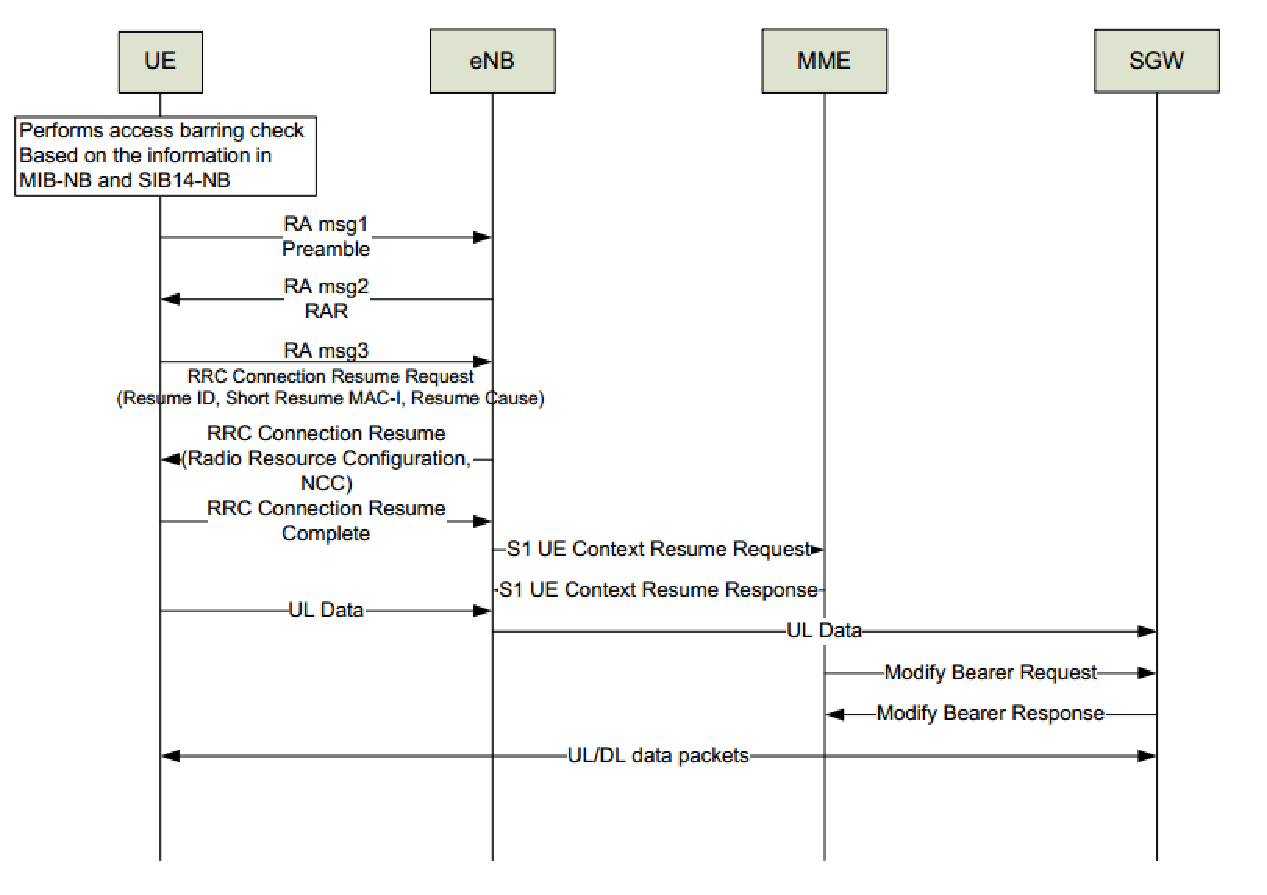
\includegraphics[width=0.8\columnwidth]{Images/dataRRCresume.pdf}
    \caption{Data transmission in RRC resume operation \cite{ratasuk2016overview}}
    \label{fig:Sequence diagram of RRC resume cycle}
\end{figure}
 %--- end of Architecture------
 


\subsubsection{Security}

The question of security for NB-IoT is very critical since data from sensor devices are sent over wireless network. The network system should be able to take care of large amount of sensitive data without causing any data loss due to network congestion, eavesdropping and, should offer proper security counter measures these high demand data. As NB-IoT devices have limited resources, they are more vulnerable to security attacks.\par

NB-IoT derive two security levels from conventional LTE,
namely: 1) AS and 2) non access stratum (NAS) security. AS establishes security between the devices and the eNB, whereas NAS security is established and managed by the devices and the mobility management entity (MME). AS and NAS provide security that are offered through ciphering and integrity algorithms listed in \cite{3GPPsecurity}. Specifically, 3GPP defines four ciphering algorithms, referred as EPS encryption algorithm (EEAs), and four integrity algorithms, referred as EPS integrity algorithm (EIA).The security configuration is performed after a negotiation between the device and, respectively, the eNB or MME. Thus, the eNB and the MME have high priority for the ciphering and integrity algorithms, which are finally selected based on the security capabilities of the device, whereas, NAS security is always configured before AS security, and both encryption and integrity algorithms are applied in NAS, the ciphering in AS is used for RRC and user plane (UP) while the integrity algorithm is applied only to RRC \cite{martinez2019exploring}.

%\subsubsection{Over the Air Update (OTA)}


\section{Related Work}\label{related work}

\subsection{Overview and Surveys}
There have been many studies on LPWAN which have described the various available LPWAN technologies and given detailed overviews and insights. In \cite{raza2017low}, the author has compared various LPWAN technologies based on technological specification, network topology, hardware cost and throughput, and in the end, the author concludes from the observation that most of the LPWAN technologies focus on MAC and physical layer and there is still a gap at the upper layer that needs to be bridged, the study also concludes by referencing that all LPWAN technologies hace their own pros and cons as per their technological principles. In general, there is not appropriate technology for specific use case. Each use case has it's own specific requirement which fits specific technology choice. In \cite{mekki2019comparative}, the author has done comparative study on three leading LPWAN technologies: Sigfox, LoRa and NB-IoT for large scale IoT deployments. Their conclusion was Sigfox and LoRa have advantage in terms of long battery life, network deployment and end device cost, while NB-IoT has benefit over in terms of QOS and latency.Similarly, in \cite{morin2017comparison}, the author has published a study on lifetime of devices for various wireless networks in Internet of Things, according to observations both Sigfox and LoRa extend the device lifetime but Sigfox matches to the mark with small payload which is valuable insight. The authors in \cite{mekki2018overview} made a comprehensive overview of the LPWAN technologies and concluded that Sigfox achieves highest network coverage among all the available LPWAN technologies.\par

\subsection{Coverage Analysis on NB-IoT and Sigfox}

Although many efforts have been put to compare the various performance parameters of the available LPWAN technologies, they are limited in the sense that most of the conclusions are based on very few or restricted number of parameters. For example, the authors in \cite{malik2019nb} produced empirical results for NB-IoT network trial, but their conclusions were based on only one performance indicator i.e., RSSI. Based on their one-factor conclusions they claimed that NB-IoT provides good connectivity in an indoor and outdoor scenario but do not provide any good performance in deep-indoor/underground scenarios. The same authors in \cite{khan2019dorm} claimed good performance of NB-IoT coverage in an indoor scenario at different elevation levels, but their conclusions were based on only two factors i.e. RSSI and SNR. Similarly, the authors in \cite{lauridsen2017coverage} produced simulation-based coverage analysis of GPRS, Sigfox, LoRa and NB-IoT for indoor and outdoor scenarios but provided no details on how these simulation-based results could be related to real-world scenarios. However, the same authors in their work \cite{vejlgaard2017coverage} compared the coverage and capacity analysis of SigFox, LoRa, GPRS, and NB-IoT  using a real site deployment covering 8000 km\textsuperscript{2} in Northern Denmark. Similarly, in \cite{nolan2016evaluation}, the author had conducted an experiment in Ireland that showed Sigfox end devices were able to communicate to the base station as far as 25 km with a RSSI as high as -145 dB.


\section{Results and Methodology}\label{Results and Methodology}

\subsection{Experimental Setup}
\begin{figure}[!h]
    \centering
    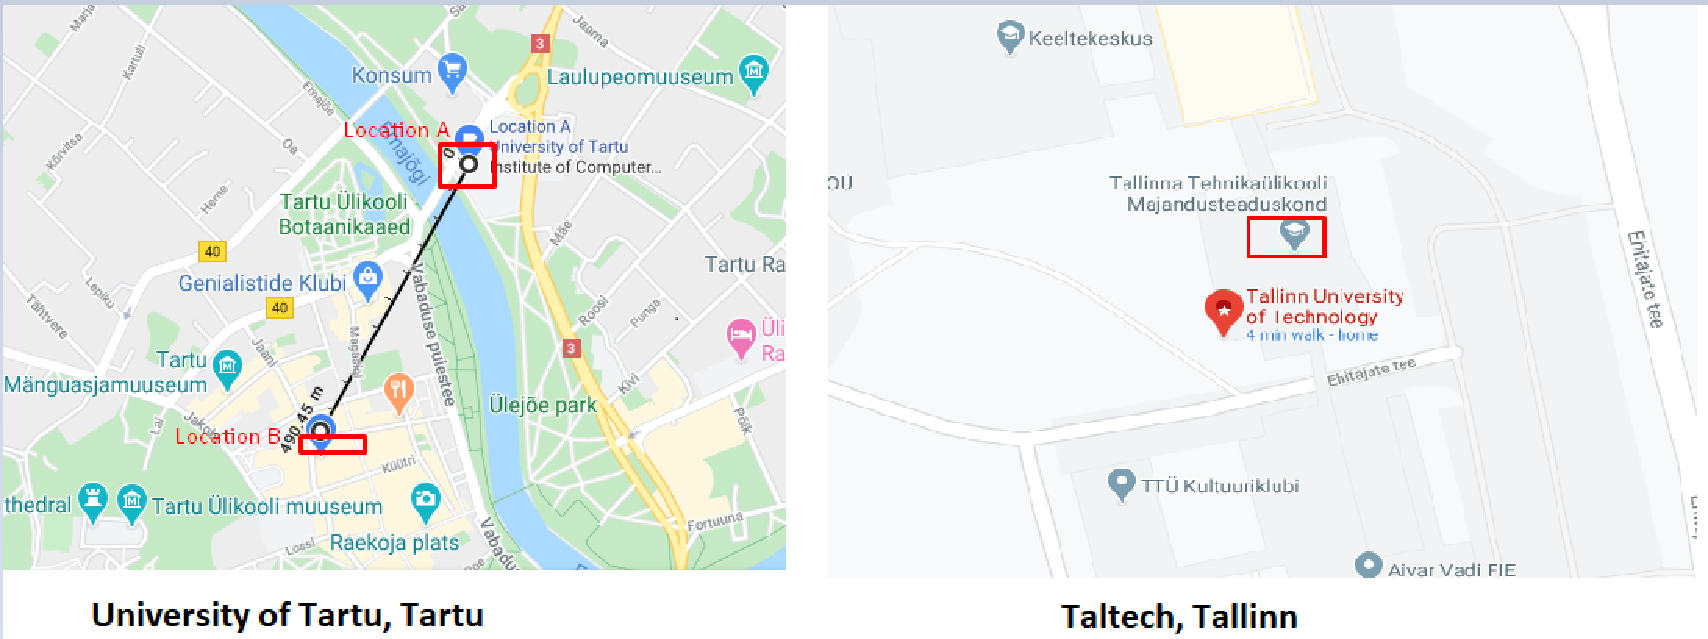
\includegraphics[width=0.9\columnwidth]{Images/locations.pdf}
    \caption{Location  of  measuring  points  in  Tartu  (Location A  and  Location  B  at  University  of  Tartu,  left)  and  Tallinn(TalTech, right)}
    \label{fig:Observation locations}
\end{figure}

During the measurement campaign in two universities i.e., University of Tartu, Delta and Paabel building, and in Tallinn University of Technology,Thomas Johann Seebeck Department of Electronics (location in Google map Figure \ref{fig:Observation locations}), a series of field tests were performed. The purpose of these field tests were to measure the RF  values i.e., RSSI in case of Sigfox and RSSI, RSRP, and RSRQ in case of NB-IoT, in three different scenarios i) Outdoor ii) Indoor,and iii) Deep-Indoor. For the analysis, below following hard-wares, devkits were utilized (see Figure \ref{fig:Experimental Setup}); discussed in below subsections respectively \ref{sigfox experimental setup} and \ref{NB-IoT experimental setup}. The measurement cycle were kept short (half-day/day), and all the measurement values were stored in a single cloud platform \\Ubidots \cite{ubidots}.

\begin{comment}


%----fig 22 deployment figures---
\begin{figure}[H]
\centering
\begin{subfigure}[t]{0.3\linewidth}
  \centering
  % include first image
  \includegraphics[width=\linewidth,origin=c,height=3cm]{images/deployment images/Outdoor.pdf}  
  \caption{Outdoor}
\end{subfigure}
\begin{subfigure}[t]{0.3\linewidth}
  \centering
  % include second image
  \includegraphics[width=\linewidth,height=3cm]{images/deployment images/Indoor.pdf}  
  \caption{Indoor}
\end{subfigure}
\begin{subfigure}[t]{0.3\linewidth}
  \centering
  % include third image
  \includegraphics[width=\linewidth, height=3cm]{images/deployment images/deep Indoor.pdf}  
\caption{Deep-Indoor}
 \end{subfigure}
\caption{Examples of deployment scenarios (a) outdoor, (b) indoor, and (c) deep-indoor}
 \label{Deployment}
\end{figure}
%---fig 22 deployment figure ends here-----

%---fig 23 experimental setup-----
\end{comment}
\begin{figure}[h]
    \centering
    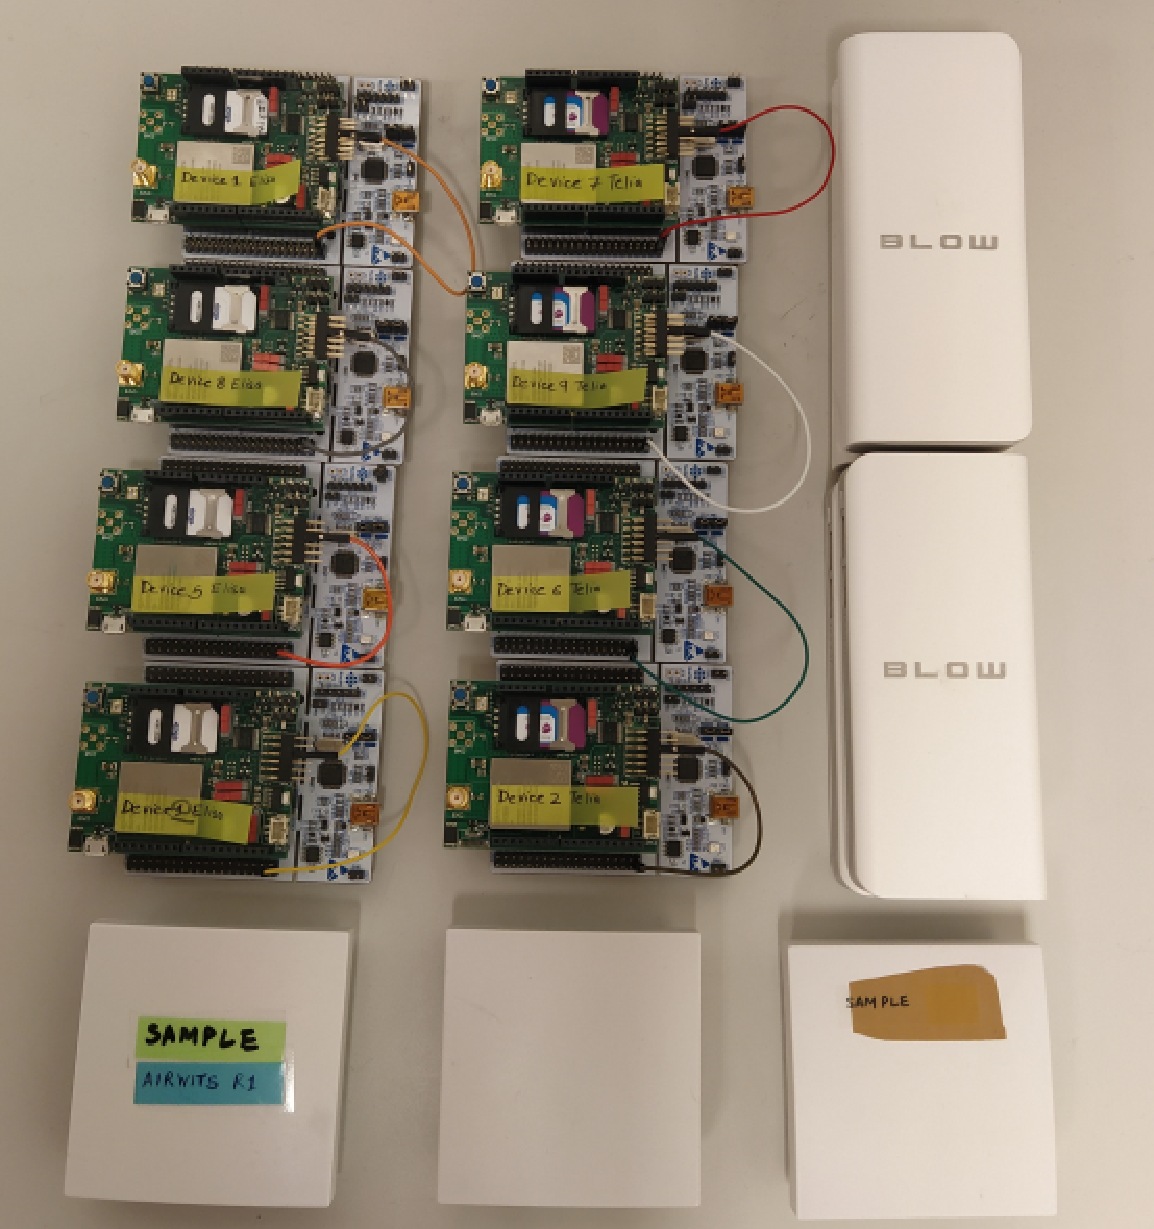
\includegraphics[trim=1cm 0cm 2cm 1cm,clip=true,width=0.9\columnwidth,totalheight=7.5cm ,width=0.9\columnwidth,keepaspectratio]{Images/experimentSetup.pdf}
    \caption{Some of the  NB-IoT (uncased) and Sigfox nodes, and batteries}
    \label{fig:Experimental Setup}
\end{figure}
%---fig 23 ends here----------



\subsubsection{Sigfox}\label{sigfox experimental setup}
For our measurement campaign,we have used proprietary Sigfox device Airwits \cite{airwits}, that is class 0, as per the specifications and has a better antenna design. Each device is deployed along with other NB-IoT nodes and transmit data to the nearest base station in every 30 minutes interval. This data upon receiving at base stations are forwarded to Sigfox core network i.e., Sigfox backend which further forwards as a callback to Ubidots \cite{ubidots} in JSON format that includes the RSSI, SNR, and the timestamps.Figure \ref{fig:Sigfox-Ubidots data flow} refers to the callback settings and Ubidots dashboard and Figure \ref{fig:Sigfox Airwits flowchart} refers to the flow chart explaining the working of the Airwits.
%---- fig 23-------
\begin{figure}[H]
  \begin{subfigure}[h]{\columnwidth}
  \centering
    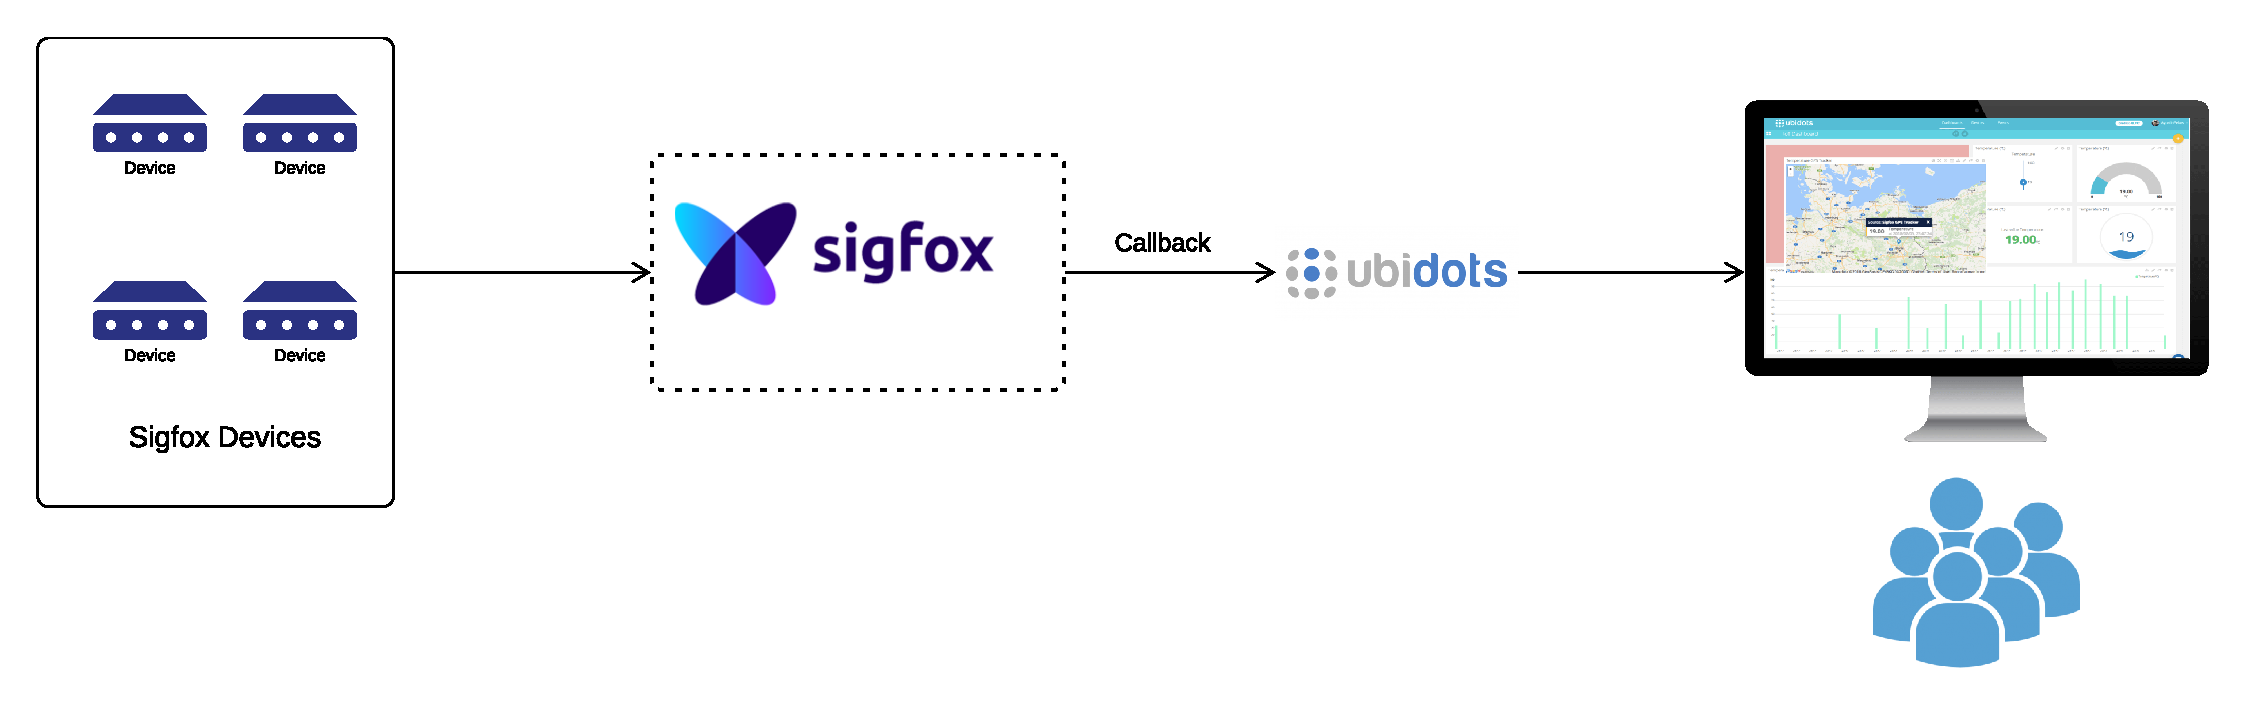
\includegraphics[width=0.8\columnwidth,height= 6cm,keepaspectratio]{Images/sigfox-ubidotsArchitecture.pdf}
    \label{fig:Sigfox and Ubidots basic architecture}
    \caption{Sigfox and Ubidots basic architecture}
\end{subfigure}
  
  \begin{subfigure}[t]{\columnwidth}
\centering
    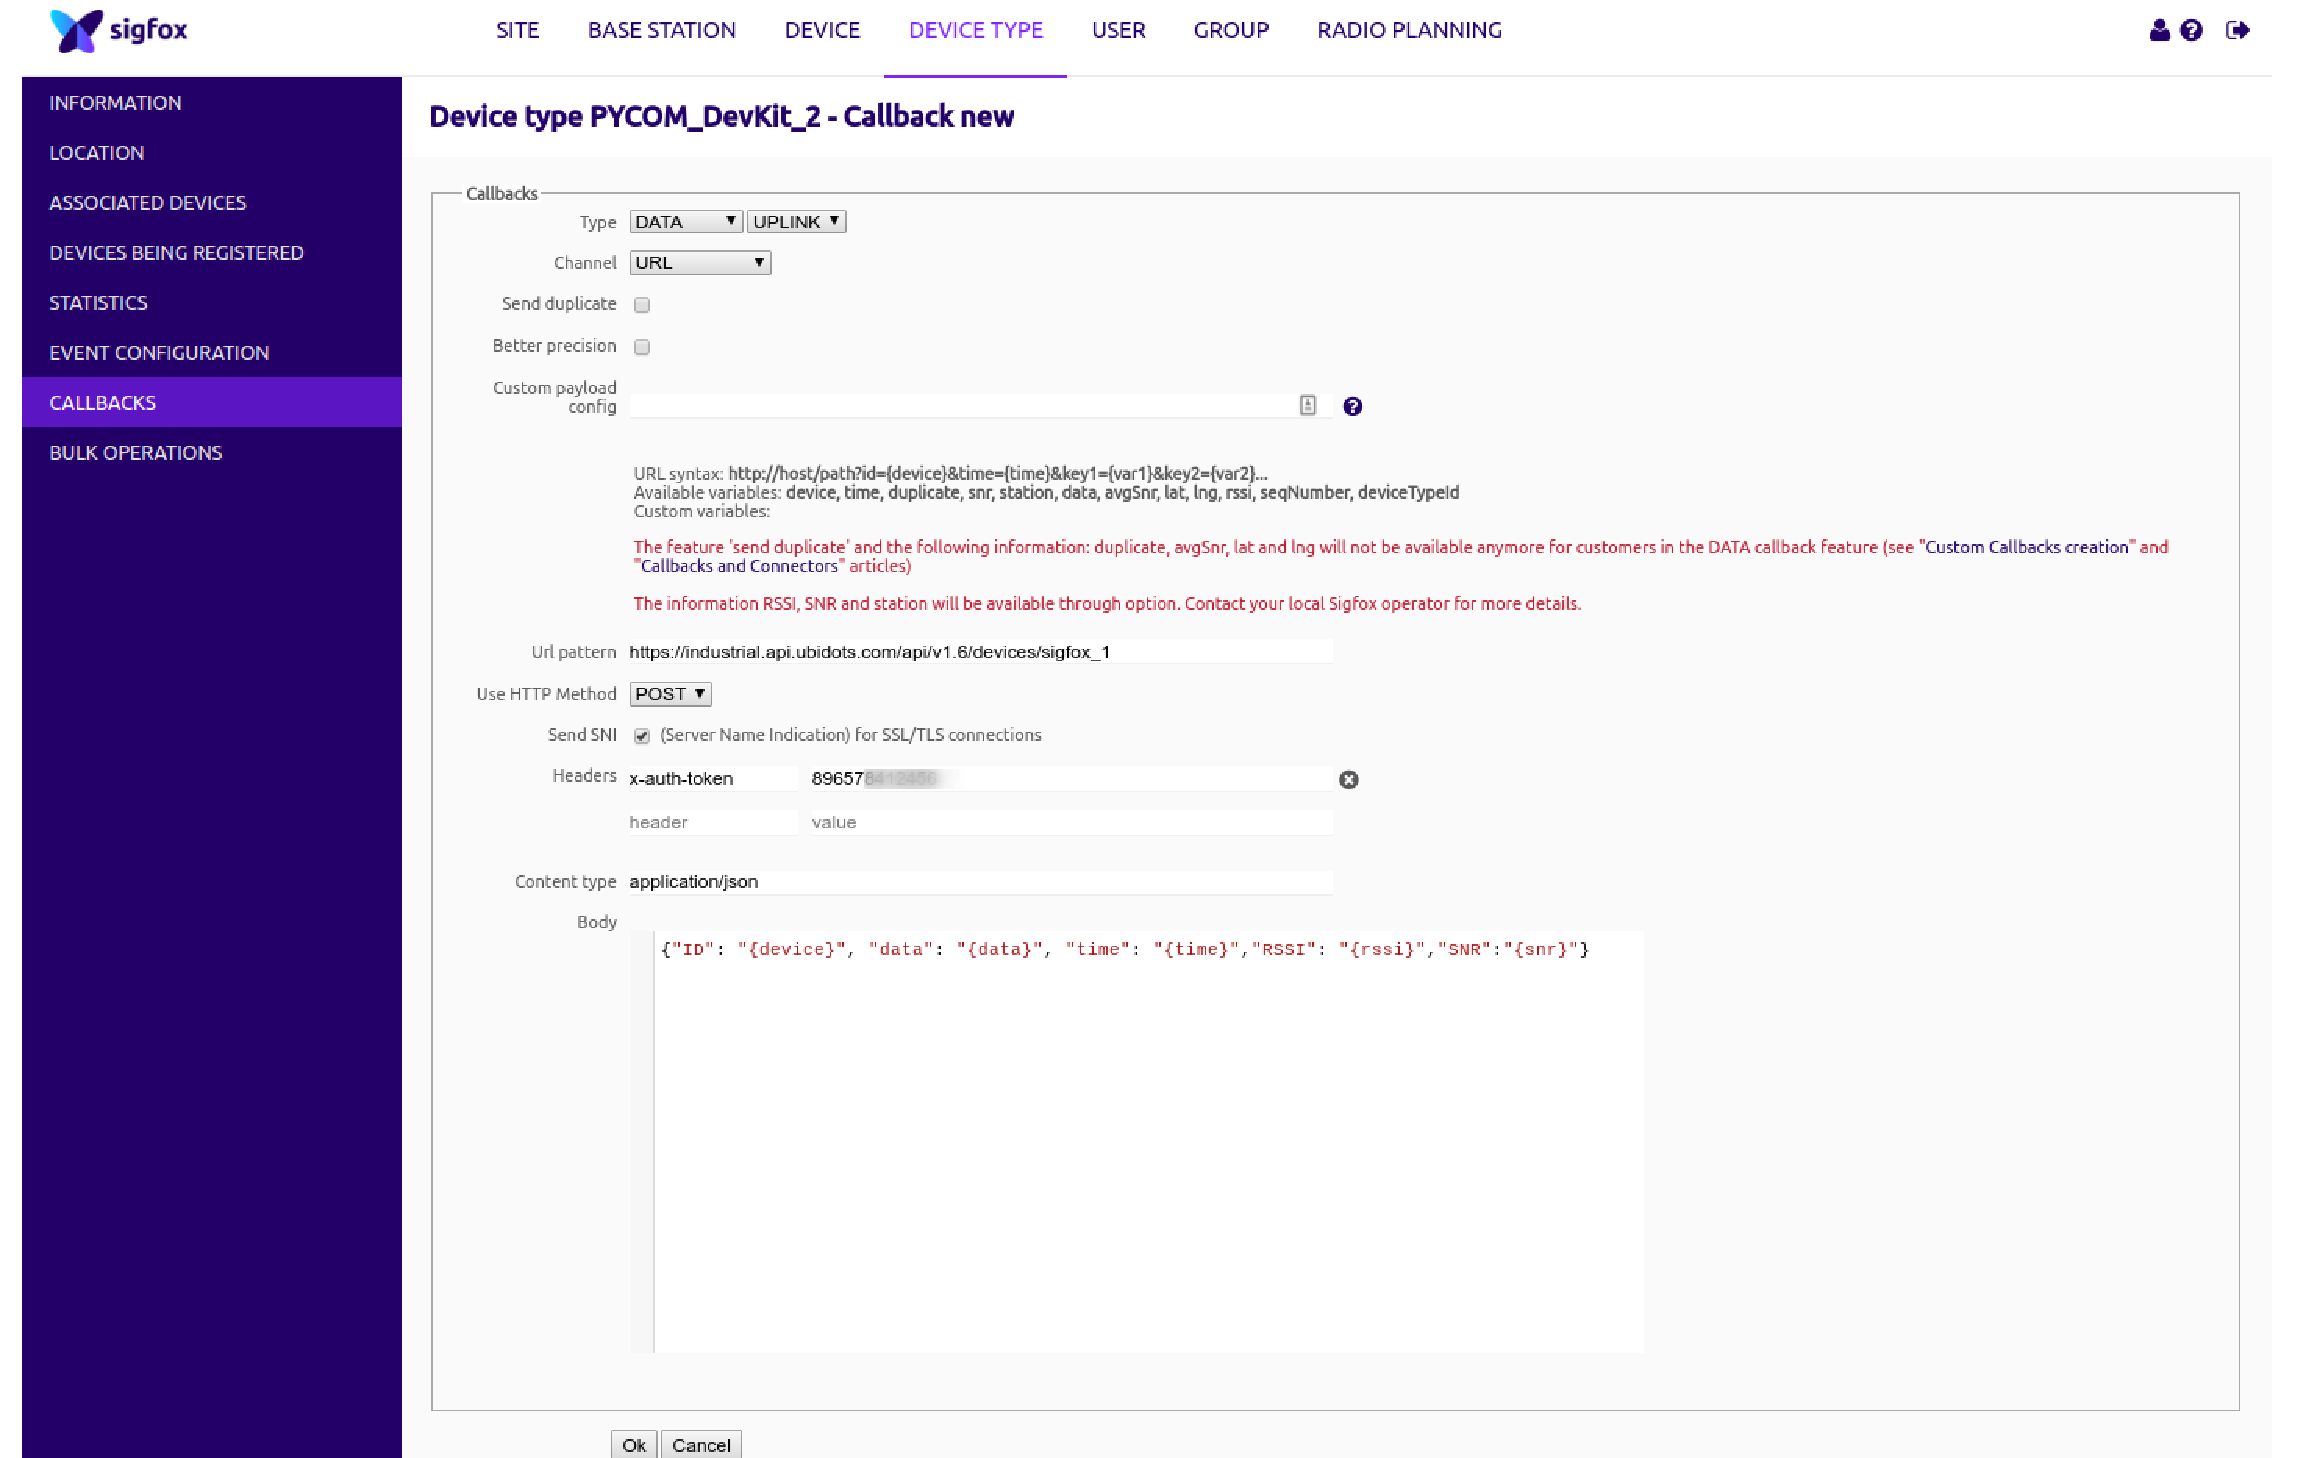
\includegraphics[trim=0.5cm 6cm 1cm 0cm,clip=true,width=0.8\columnwidth,totalheight=6cm,keepaspectratio ]{Images/SigfoxUbidotsCallback.pdf}
    \caption{Ubidots callback definition at Sigox backend}
  \end{subfigure}
  
  
  \begin{subfigure}[t]{\columnwidth}
\centering
    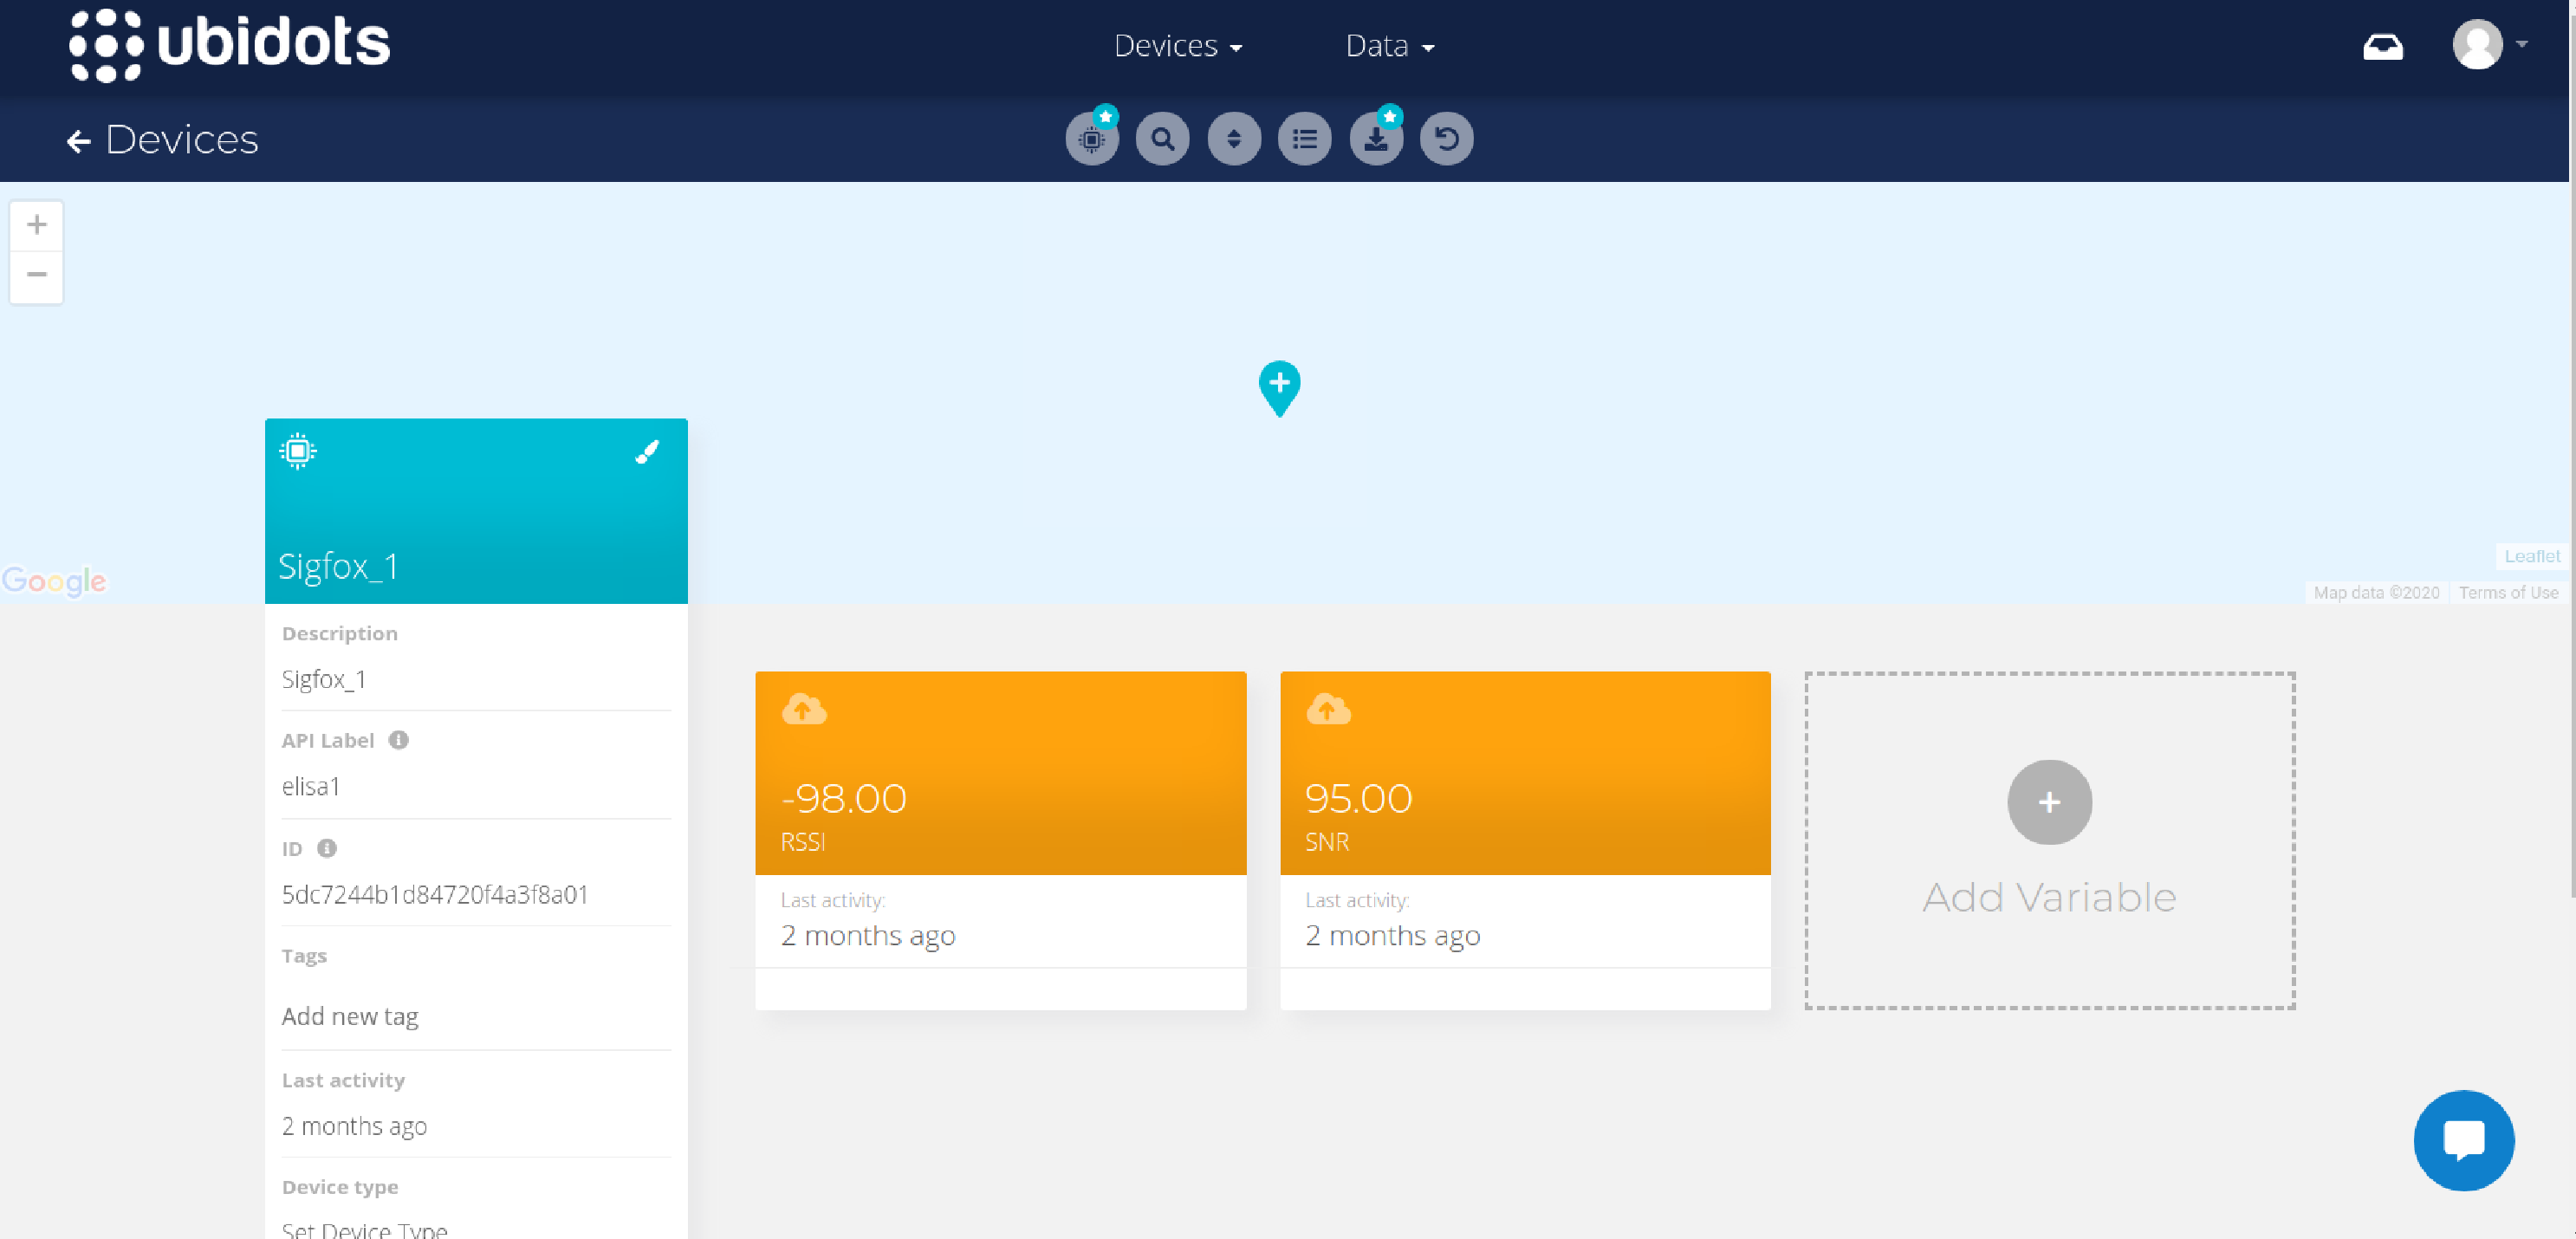
\includegraphics[trim=0.5cm 1cm 2cm 0cm,clip=true,width=0.8\columnwidth,totalheight=6cm,keepaspectratio ]{Images/UbidotsDashboard.pdf}
    \caption{Ubidots dashboard with RF parameters}
  \end{subfigure}
  
    \caption{Sigfox-Ubidots data flow}
    \label{fig:Sigfox-Ubidots data flow}
\end{figure}
%---- fig 23 ends here----



%---Fig 24 Airwits flow chart
\begin{figure}[H]
    \centering
    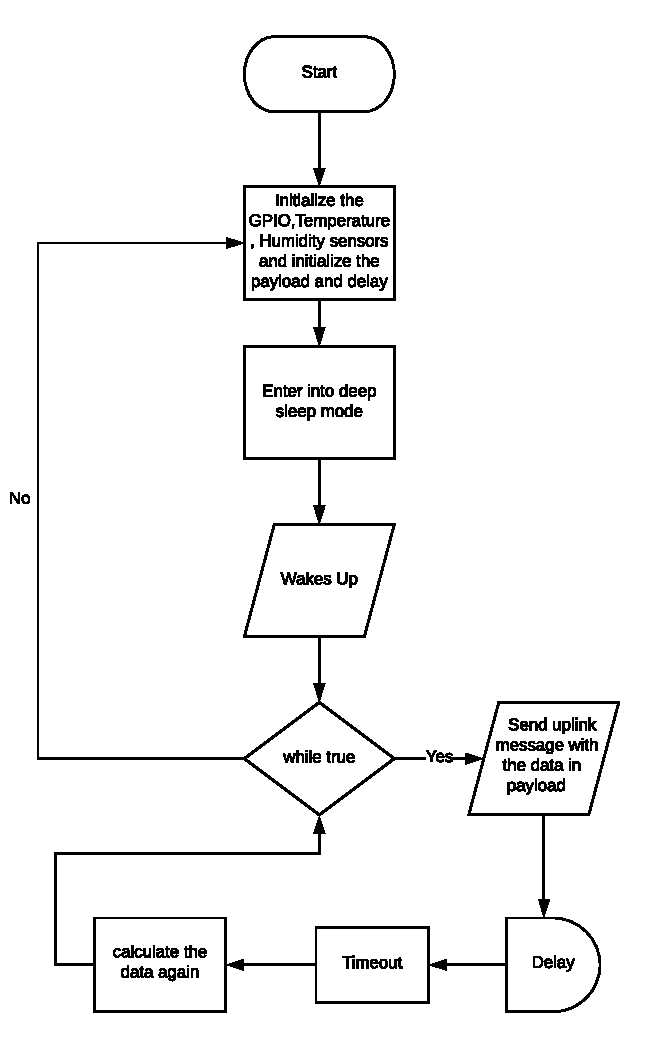
\includegraphics[width=0.9\columnwidth,height=10cm,keepaspectratio]{Images/AirwitsFlowchart.pdf}
    \caption{Sigfox Airwits flowchart}
    \label{fig:Sigfox Airwits flowchart}
\end{figure}
%---fig 25 ends here--------



\subsubsection{NB-IoT}\label{NB-IoT experimental setup}
For our measurement campaign, we have used the Avnet Silica NB-IoT shield which is embedded with Quectel BG96 radio chipset that features ultra-low power consumption and supports various communication channels i.e., LTE CAT NB1 (i.e. 3GPP Release 13 NB-IoT) along with other standard interfaces such as USB/UART/I2C/Status Indicator) \cite{avnetBG96}. The shield is combined with the STM32 based micro-controller, i.e., Nucleo-L476RG(CORTEX M4) \cite{STM} which is used as the processing unit as they are highly affordable and at the same time can be combined with wide varieties of sensors. Figure \ref{fig:NB-IoT node with Avnet BG96 shield and STM-32 L476RG micro-controller} illustrates the working setup of NB-IoT which is powered by 20,000 mAh external battery. \par

%----fig 25 -------------
\begin{figure}[H]
    \centering
    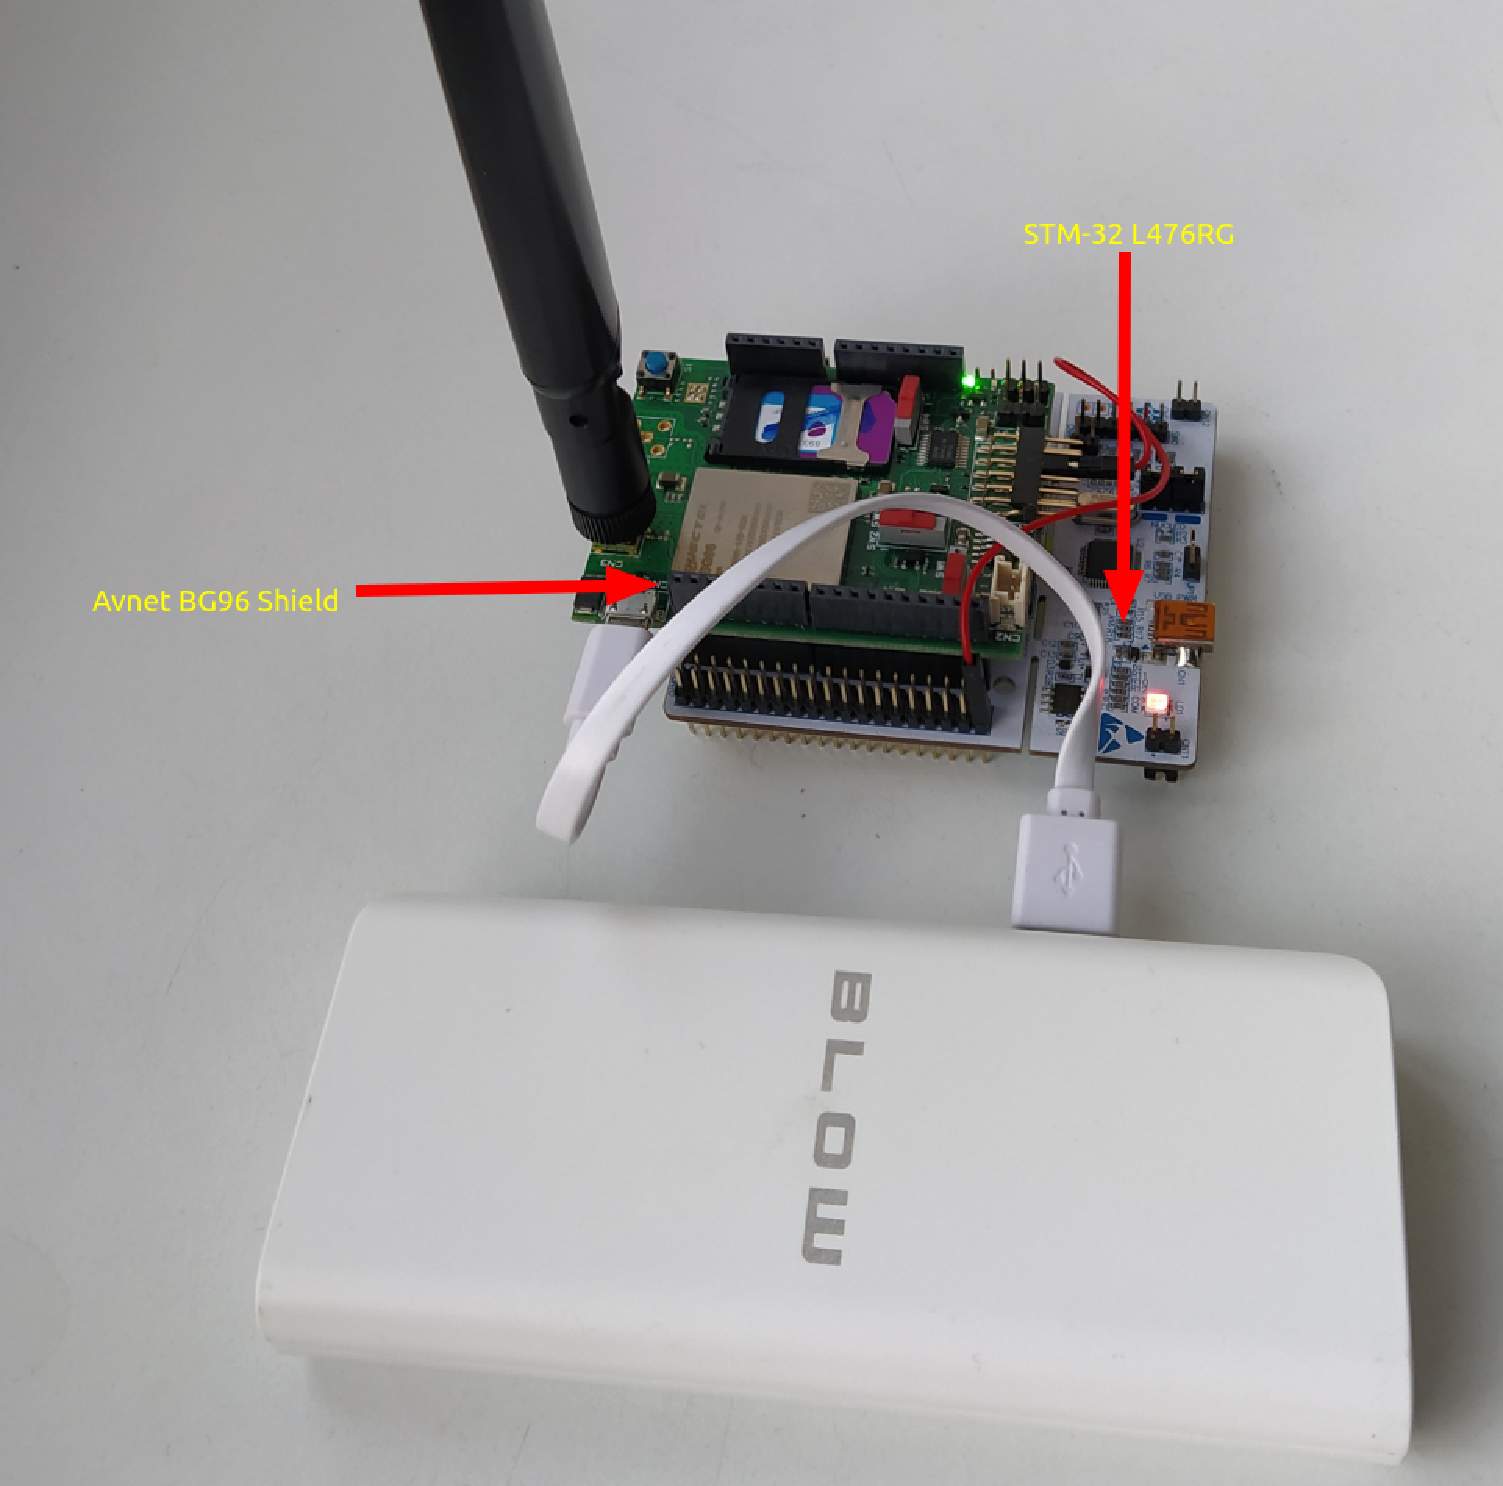
\includegraphics[trim=1cm 0cm 2cm 1cm,clip=true,width=0.9\columnwidth,totalheight=8cm ,width=0.9\columnwidth,keepaspectratio]{Images/nb-iotNode.pdf}
    \caption{NB-IoT node with Avnet BG96 shield and STM-32 L476RG micro-controller}
    \label{fig:NB-IoT node with Avnet BG96 shield and STM-32 L476RG micro-controller}
\end{figure}
%-----fig25 ends here------

These nodes are inserted with NB-IoT SIM cards from the two different NB-IoT operators (referred to as Operator A and Operator B in the rest of this thesis), and are programmed to send the RF parameters to Ubidots \cite{ubidots} at 30 minutes interval containing RSSI, SNR, RSRP, RSRQ, and RSRP. The algorithm of the node is designed such a way that it goes into power saving mode (deep-sleep) after transmitting the the packet, thus saving the battery.The working of these nodes are explained by the help of flow chart, see Figure \ref{fig:NB-IoT node code flowchart diagram}. 


%---fig 26 ---nbiot flowchart----
\begin{figure}[H]
    \centering
    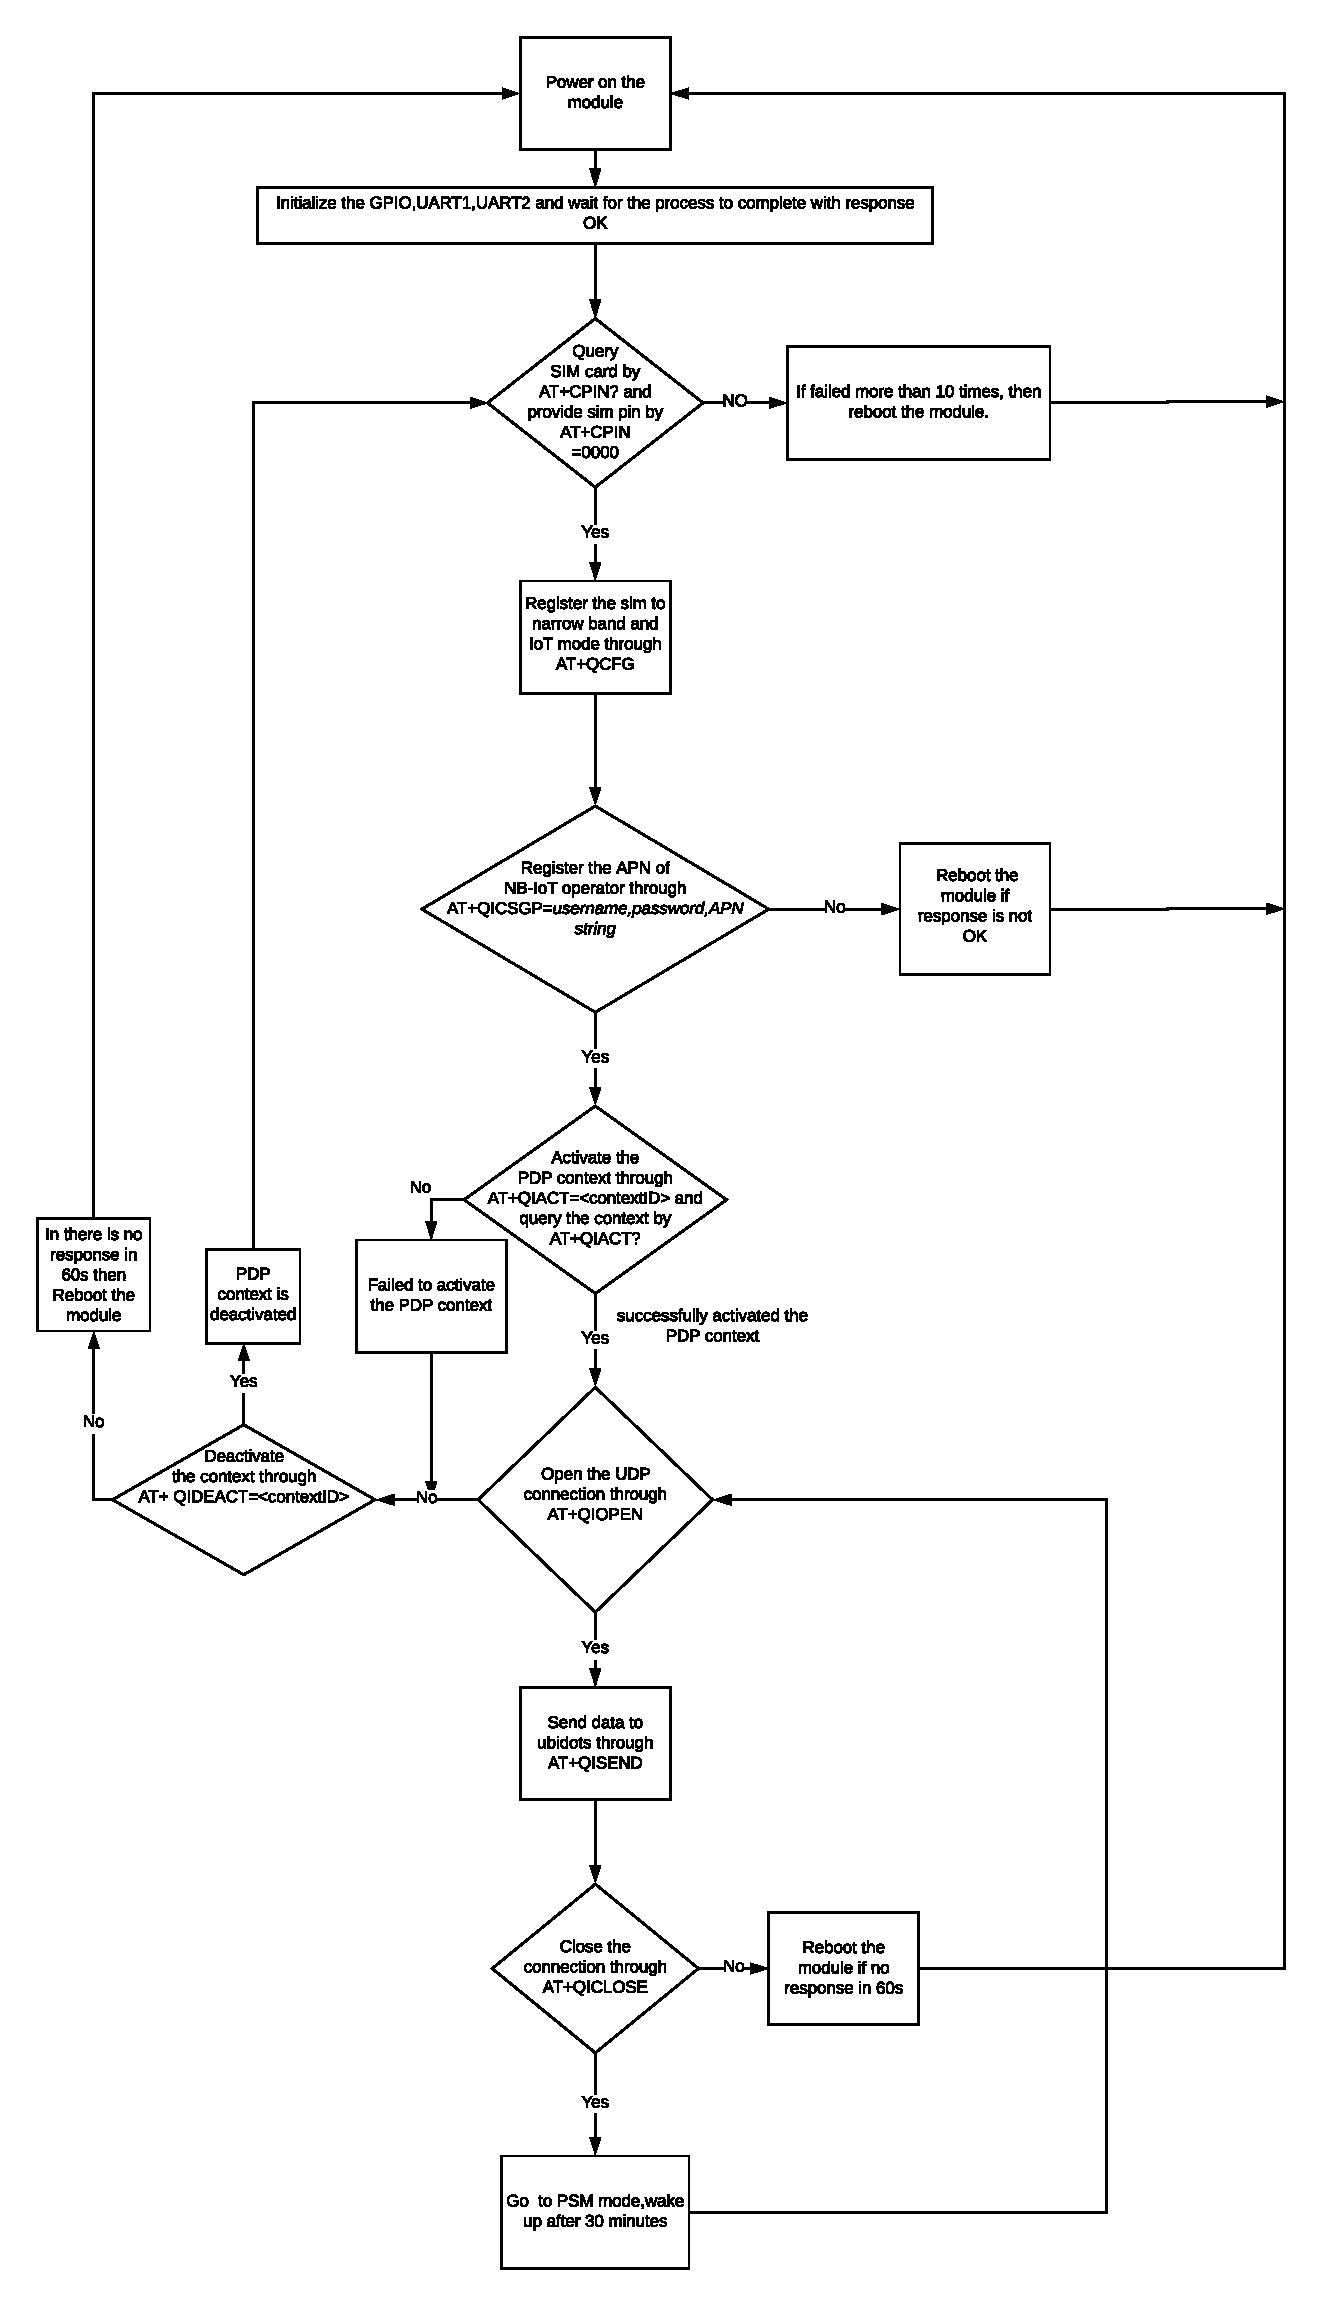
\includegraphics[width=0.5\columnwidth,height=12cm]{nbiotFlowchart.pdf}
    \caption{NB-IoT node code flowchart diagram}
    \label{fig:NB-IoT node code flowchart diagram}
\end{figure}
%---fig 27 nbiot flow chart ends here---

\subsection{Results}\label{results}

This section evaluates the RF results of Sigfox and NB-IoT in three different scenarios i) Outdoor ii) Indoor, and iii) Deep-Indoor/Basement in two University campuses, University of Tartu and TalTech as aforementioned. The radio coverage depends on link budget and other radio parameters for e.g., transmission power, connector loss, antenna gain, the height of antenna that directly affects the overall coverage. Factors like free space path loss, fading reflection, refraction, building structure, and Fresnel zone also affects the coverage \cite{sikora2019test,sikora2019performance}. Therefore, results are outlined on the basis of 3-factor analysis by considering i) RSSI ii) RSRP and iii) RSRQ of the received signal as explained briefly below. Further, these RF metrics i.e., RSSI, RSRP and RSRQ are categorized into four distinct classes of link quality: POOR, FAIR, GOOD and EXCELLENT. The exact corresponding values differ for NB-IoT and Sigfox in the results; the respective values have been detailed in Tables \ref{nbiotRSSI}-\ref{sigfoxRSSI} for RSSI;  Table \ref{nbiotRSRP} for RSRP; and Table \ref{nbiotRSRQ} for RSRQ and Table \ref{nbiotSINR} for SINR.


\paragraph{RSSI:}
Received Signal Strength Indicator (RSSI) or "Total  Power", is the radio  signal  strength  within  the  receive bandwidth. It is usually the power received by antenna, and is  calculated in dBm using an equation \ref{RSSI} \cite{3GPP}.

\begin{equation}
      RSSI = {12 \times N \times RSRP}
      \label{RSSI}
\end{equation}
Where, N= Number of PRBs and RSRP is reference signal received power.

%----table 4----
\begin{table}[h]

\centering
\caption {RSSI reference values for NB-IoT as per 3GPP standards \cite{3GPP,sikora2019performance}}

\begin{tabular}{|p{5cm}|p{5cm}|}
\hline
\multicolumn{2}{|c|}{NB-IoT RSSI REFERENCES} \\ \hline
 > −65 dBm                           & EXCELLENT                     \\ \hline
−65 to −75 dBm                      & GOOD                          \\ \hline
−75 to −85 dBm                      & FAIR                          \\ \hline
< -85 dBm                           & POOR                          \\ \hline
\end{tabular}
\label{nbiotRSSI}

\end{table}
%----table 4 ends here----


%----table 5-------
\begin{table}[H]
\caption {RSSI reference values for Sigfox \cite{sigfoxRSSI}}
\centering
\resizebox{0.744\columnwidth}{!}{
\begin{tabular}{|c|c|}
\hline
\multicolumn{2}{|c|}{SIGFOX RSSI REFERENCES} \\ \hline
> -122dBm                    & EXCELLENT     \\ \hline
-135dBm < RSSI ≤ -122dBm     & GOOD          \\ \hline
-122dBm < RSSI               & GOOD          \\ \hline
\begin{tabular}[c]{@{}c@{}}-135dBm < RSSI ≤ -122dBm\\ (if data received by 1 or 2 base stations)\end{tabular} & FAIR \\ \hline
RSSI ≤ -135dBm               & POOR          \\ \hline
\end{tabular}}
\label{sigfoxRSSI}
\end{table}

%----table 5 ends here----

\paragraph{RSRP:}
Reference Signal Received Power (RSRP) is similar to RSSI and refers to the average received power over the resource elements that carry cell-specific reference signals within  certain  frequency  bandwidth. RSRP is applicable to RRC\_idle and RRC\_connected  states. It is measured in dBm and is calculated using the equation \ref{RSRP equation}.

\begin{equation}
    RSRP = {{RSSI - 10\times log (12\times N) }}
    \label{RSRP equation}
\end{equation}
Where, 
\begin{itemize}
    \item N = Number of PRBs 
    \item RSSI= Received Signal Strength Indicator(explained above).
\end{itemize}



%---table 6-----
\begin{table}[h]
\caption {RSRP reference values for NB-IoT as per 3GPP standards \cite{3GPP,sikora2019performance}}
\centering

\begin{tabular}{|p{5cm}|p{5cm}|}
\hline
\multicolumn{2}{|c|}{NB-IoT RSRP REFERENCE} \\ \hline
> −84 dBm                            & EXCELLENT                    \\ \hline
−85 to −102 dBm                      & GOOD                         \\ \hline
−103 to −111 dBm                     & FAIR                         \\ \hline
< -112                               & POOR                         \\ \hline
\end{tabular}
\label{nbiotRSRP}
\end{table}

%---table 6 ends here-----



It should be noted in the below results that at higher values of RSRP, the BG96 has not calculated the RSSI, it should not be interpreted as packet loss; the same characteristics have been observed in other radio modules e.g., SARA-N210 \cite{basu2019experimental}, therefore the graphs below have breaks in RSSI values. Therefore, RSRP is a more suitable parameter to be considered. Nevertheless, we have tried to analyse the corresponding RSSI measurement as well whenever possible.

\paragraph{RSRQ:}
Reference Signal Received Quality (RSRQ) indicates the quality of received reference signal and is applicable only in RRC\_connected state. It is calculated in dB as per equation \ref{RSRQ equation}. 
\begin{equation}
     RSRQ= {{N\times} RSRP/ RSSI}
     \label{RSRQ equation}
\end{equation}
\\ Where,
\begin{itemize}
    \item N: indicates the number of PRBs.
\end{itemize}

%---table 7 ----
\begin{table}[!h]
\caption {RSRQ reference values for NB-IoT as per 3GPP standards\cite{3GPP,sikora2019performance}}
\centering

\begin{tabular}{|p{5cm}|p{5cm}|}
\hline
\multicolumn{2}{|c|}{NB-IoT RSRQ REFERENCE} \\ \hline
>−5 dB                 & EXCELLENT          \\ \hline
-5 to -8 dB            & GOOD               \\ \hline
-8 to -11 dB           & FAIR               \\ \hline
< -11 dB               & POOR               \\ \hline
\end{tabular}

\label{nbiotRSRQ}
\end{table}
%---table 7 ends here ----

\paragraph{SINR:} Signal to Interference Noise Ratio, is the ratio of signal power and the noise power. It is measured in dB, and calculated using the equation \ref{SINR equation}. \par

\begin{equation}
       SINR={\dfrac{P}{(I+N)}}
     \label{SINR equation}
\end{equation}
where, 
\begin{itemize}
    \item P: indicates the power of reference signal
    \item I: indicates the average interference power
    \item N: indicates the number of PRBs
\end{itemize}

%---table 8 SINR ----
\begin{table}[H]
\caption {SINR reference values for NB-IoT as per 3GPP standards\cite{3GPP,sikora2019performance}}
\centering

\begin{tabular}{|p{5cm}|p{5cm}|}
\hline
\multicolumn{2}{|c|}{NB-IoT SINR REFERENCE} \\ \hline
> 12 dB                 & EXCELLENT          \\ \hline
10 to 12.5 dB            & GOOD               \\ \hline
7 to 10 dB           & FAIR               \\ \hline
< 7 dB               & POOR               \\ \hline
\end{tabular}

\label{nbiotSINR}
\end{table}
%---table 8 ends here ----

Furthermore, the results have been categorised below into three subsections based on the above three deployment scenarios.

\subsubsection{Coverage Analysis in Outdoor Scenario}\label{Outdoor Analysis}

The test-beds were deployed in outside locations of both campuses. Specifically, in case of UT, devices were deployed on the roof top of Delta building; in TalTech campus, devices were deployed in outside campus ground as can be seen in the Figure \ref{fig:Outdoor deployment}.\par



%---figure 28----
\begin{figure}[h]
\centering
\begin{subfigure}[t]{0.42\linewidth}
  \centering
  % include first image
   \includegraphics[width=6cm,height=6cm,angle=-90]{Images/sitePictures/Tartu/outdoor.jpg} 
  \caption{UT outdoor scenario}
\end{subfigure}
\begin{subfigure}[t]{0.42\linewidth}
  \centering
  % include second image
  \includegraphics[height=6cm,width=6cm,angle=-90]{Images/sitePictures/Tallinn/outdoor.jpg} 
  \caption{TalTech outdoor scenario}
\end{subfigure}

\caption{Outdoor deployment}
 \label{fig:Outdoor deployment}
\end{figure}
%---figure 28 ends here----








%----figure 29 tartu outside-----

\begin{figure}[!h]
\begin{subfigure}[t]{\linewidth}
  \centering
  % include first image
  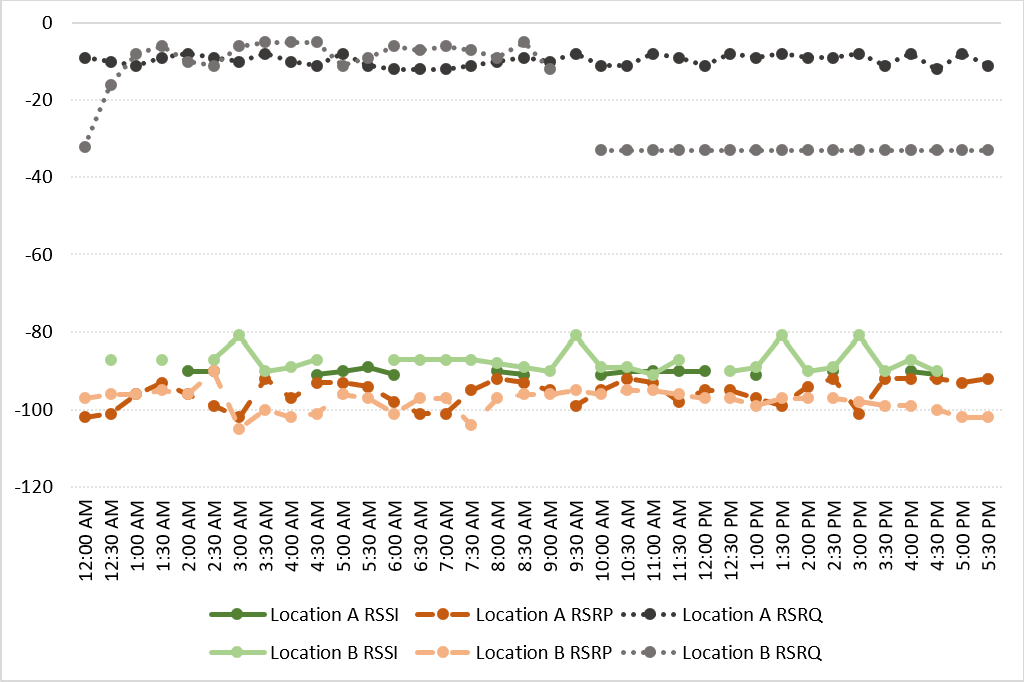
\includegraphics[width=.5\linewidth]{Images/tartu/ATartuOut.pdf}  
  \caption{NB-IoT Operator A}
\end{subfigure}
\begin{subfigure}[t]{\linewidth}
  \centering
  % include second image
  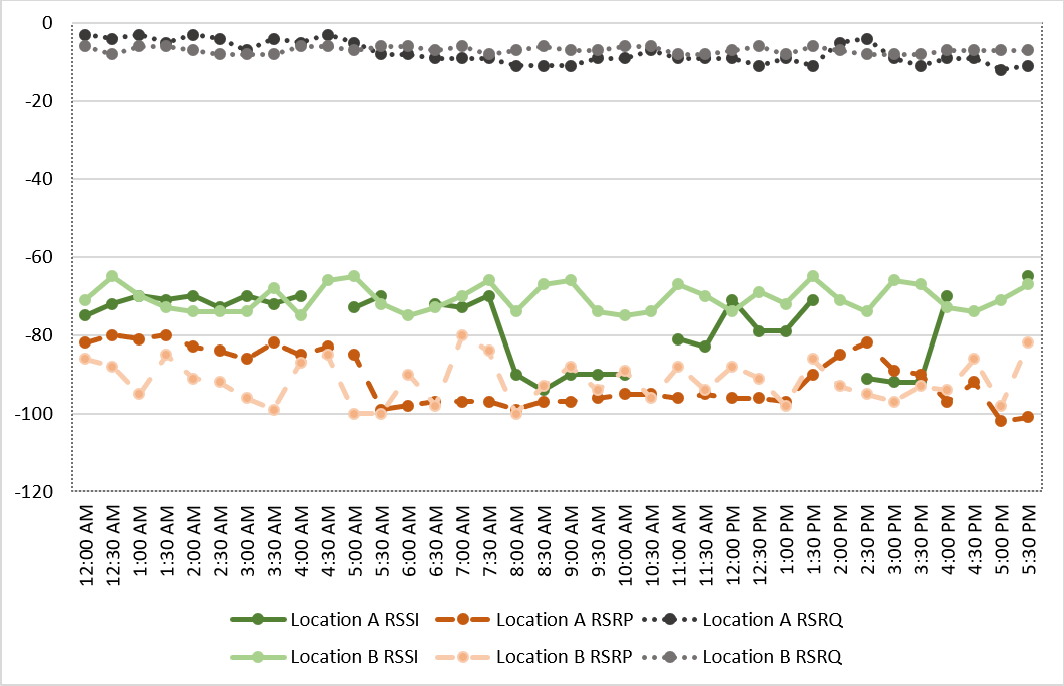
\includegraphics[width=.5\linewidth]{Images/tartu/BTartuOut.pdf}  
  \caption{NB-IoT Operator B}
\end{subfigure}

\begin{subfigure}[t]{\linewidth}
  \centering
  % include third image
  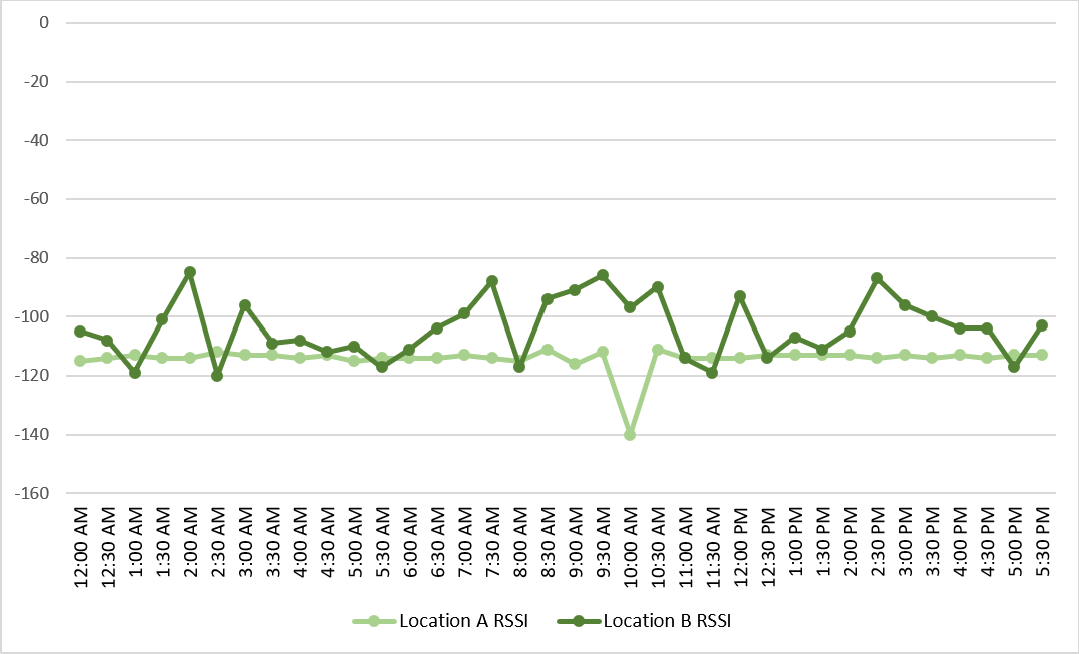
\includegraphics[width=.5\linewidth]{Images/tartu/STartuOut.pdf}  
\caption{Sigfox}
 \end{subfigure}
\caption{RF coverage and signal quality: outdoor scenario at University of Tartu}
 \label{RFOutdoor UT}
\end{figure}
%---figure 29 ends here-----


%---figure 30 tallinn outdoor ---
\begin{figure}[!h]
\begin{subfigure}[t]{\linewidth}
  \centering
  % include first image
  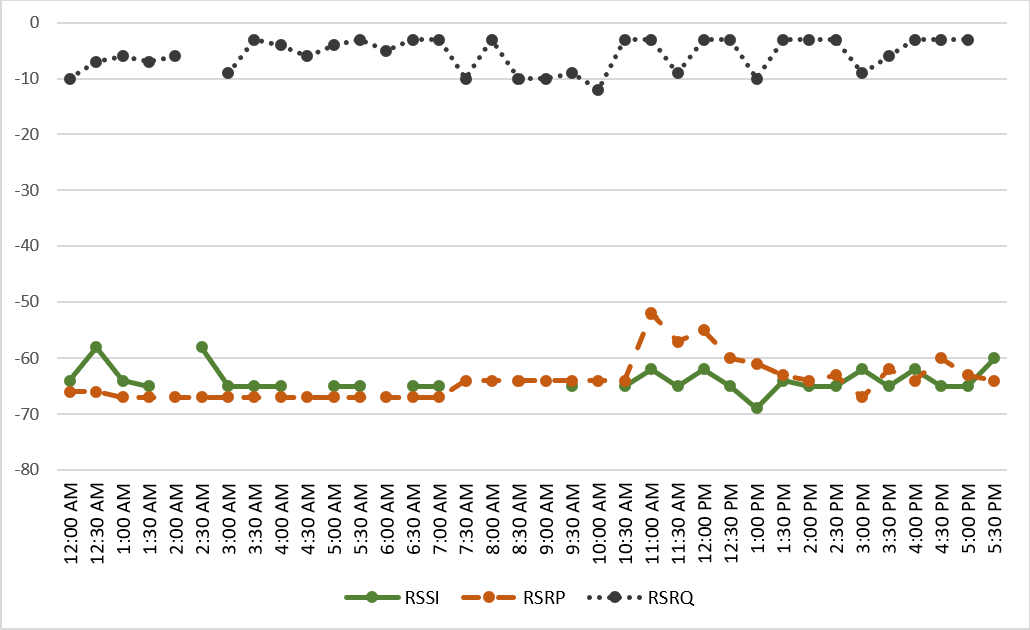
\includegraphics[width=.5\linewidth]{Images/tallinn/ATallinnOut.pdf}  
  \caption{NB-IoT Operator A}
\end{subfigure}
\begin{subfigure}[t]{\linewidth}
  \centering
  % include second image
  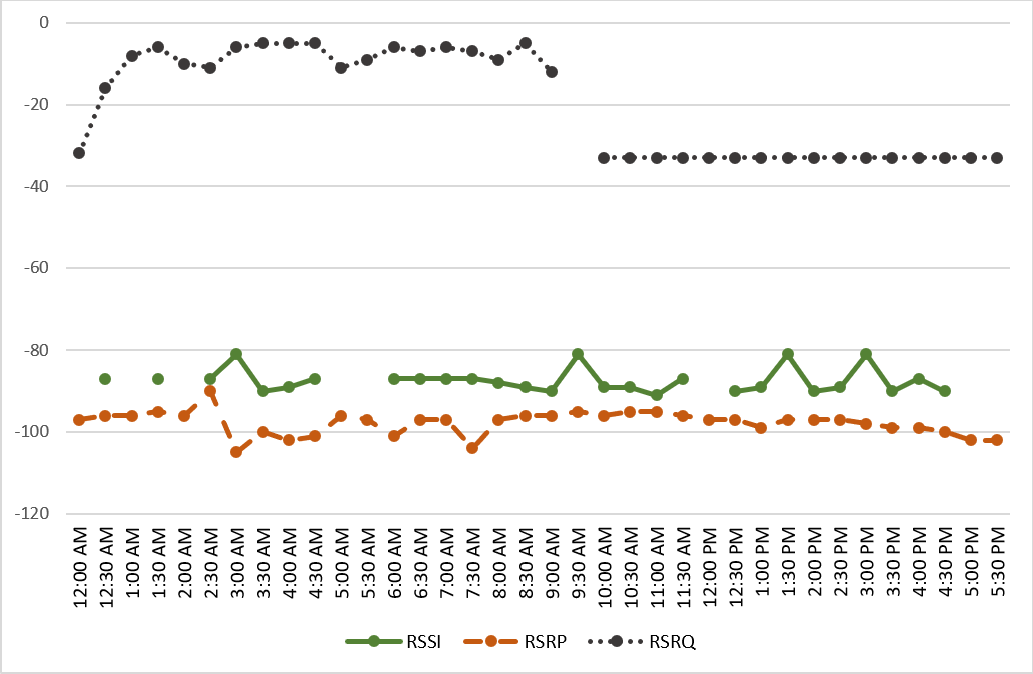
\includegraphics[width=.5\linewidth]{Images/tallinn/BTallinnOut.pdf}  
  \caption{NB-IoT Operator B}
  
\end{subfigure}
\begin{subfigure}[t]{\linewidth}
  \centering
  % include third image
  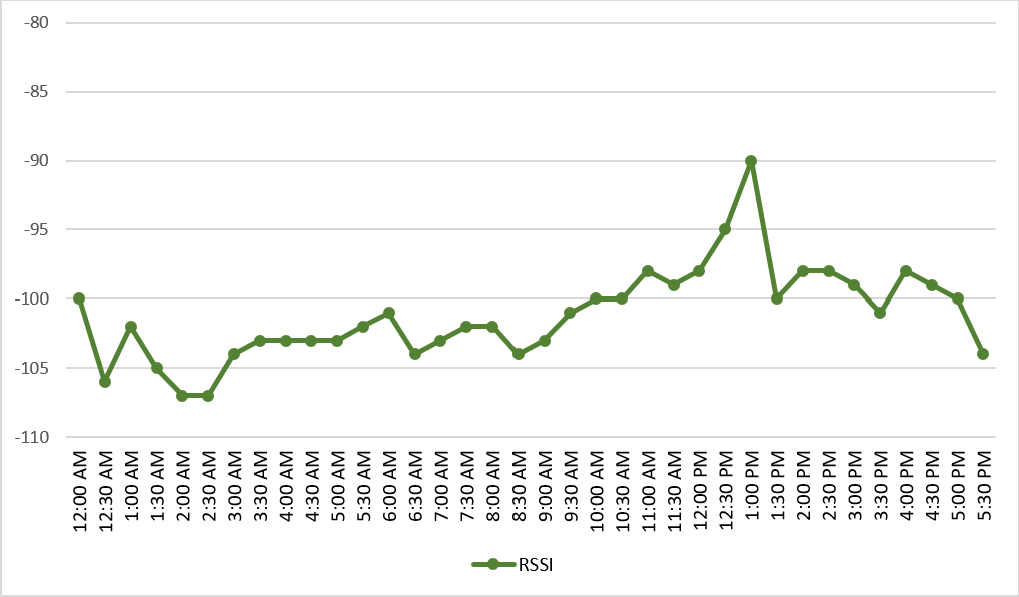
\includegraphics[width=.5\linewidth]{Images/tallinn/STallinnOut.pdf}  
\caption{Sigfox}
 \end{subfigure}
\caption{RF coverage and signal quality: outdoor scenario at TalTech}
 \label{RFOutdoor Taltech}
\end{figure}
%---figure 30 tallinn outdoor ends here ---

%-- figure 31 RSRP Boxplot figure
 \begin{figure}[h!]
\begin{subfigure}[t]{\linewidth}
  \centering
  % include first image
  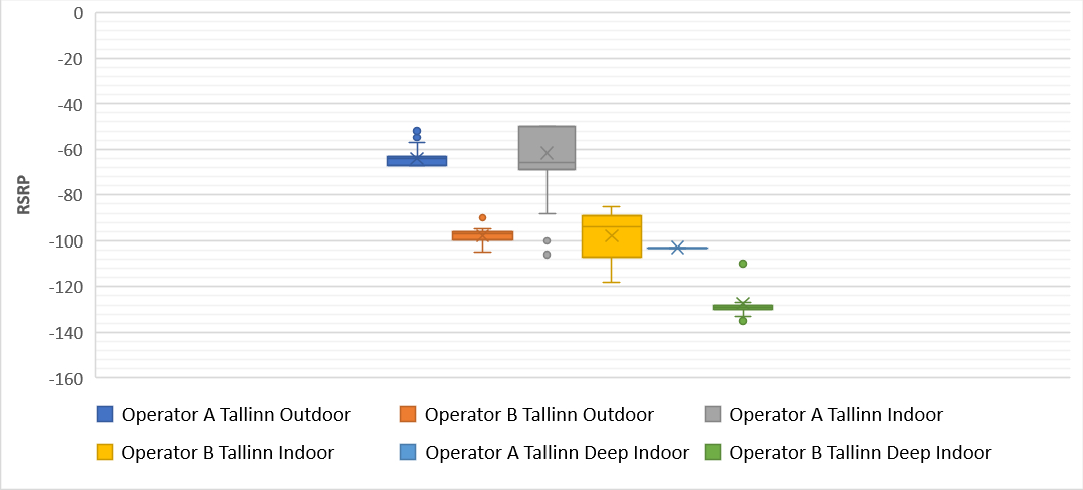
\includegraphics[width=.5\linewidth]{Images/tallinn/TallinnRSRPboxplot.pdf}  
  \caption{TalTech campus, Tallinn}
\end{subfigure}
\begin{subfigure}[t]{\linewidth}
  \centering
  % include second image
  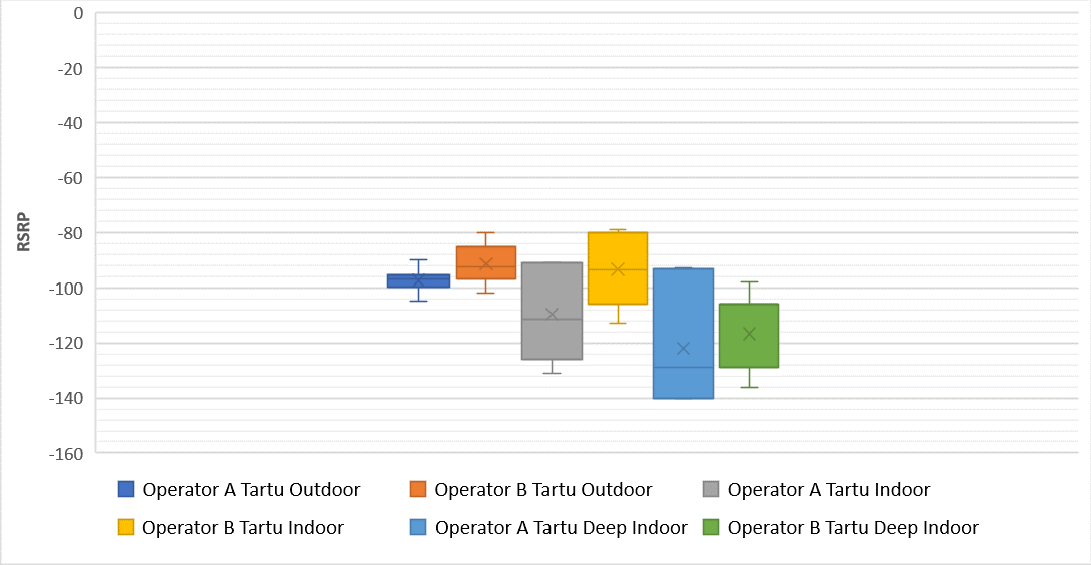
\includegraphics[width=.5\linewidth]{Images/tartu/TartuRSRPboxplot.pdf}  
  \caption{University of Tartu campus, Tartu}
  
\end{subfigure}
\caption{NB-IoT RSRP distribution in Tallinn and Tartu}
 \label{boxplot}
\end{figure}
%-----figure 31 end here-----

Furthermore, Figure \ref{RFOutdoor UT} presents the RF coverage results  in $University\ of\  Tartu$ in Locations A and B (refer to Fig. \ref{fig:Observation locations} to see locations on map). During the analysis, it was observed that $operator\ B$ has slightly better outdoor coverage than $operator\ A $ with average RSRP -91.2 dBm compared to -97.4 dBm, as shown in Figure \ref{boxplot}. For RSSI, $operator\ B$ has shown good performance with average RSSI of -77 dBm at location A and -69 dBm RSSI recorded at location B, compared to -90 dBm and -87 dBm, respectively, in case of $operator\ A$. On the other hand, for Sigfox the average RSSI values recorded at Locations A and B were -114 dBm and -103 dBm respectively, which reflects excellent coverage as per \cite{sigfoxRSSI}. For RSRQ, which is defined as quality of received signal \cite{3GPP}, $Operator\ A$ has showed lower RSRQ index at location B compared to $operator\ B$ which shows the weak coverage of $operator\ A$ at this location.\par
%----figure 30 tartu outdoor----



In addition to the above, in $Taltech$ Figure \ref{RFOutdoor Taltech}, $operator\ A$ has good coverage with average RSSI value -64 dBM whereas $operator\ B$ has fair coverage with average RSSI value -87 dBm. Similar to RSSI, other parameters RSRP and RSRQ showed similar patterns for $operator\ A$ having median RSRP value -64 dBm compared to -97 dBm in case of $operator\ B$, refer to Figure \ref{boxplot}, and Sigfox on the other hand has good RSSI strength with -101 dBm which reflects excellent coverage as per Table \ref{sigfoxRSSI}.\par
It is important to highlight NB-IoT and Sigfox both had 0\% packet loss for the outdoor scenario.




\subsubsection{Coverage Analysis in Indoor Scenario}
To observe the indoor coverage, test-beds were deployed in 3\textsuperscript{rd} floor of UT's , Delta and Paabel building and similar setup was deployed at 1\textsuperscript{st} and 2\textsuperscript{nd} floor of TalTech's Thomas Johann Seebeck Department of Electronics (see Figure \ref{fig:Indoor deployment}).


%---Figure 32 Indoor deployment-----
\begin{figure}[h!]
\centering
\begin{subfigure}[t]{0.42 \linewidth}
  \centering
  \includegraphics[width=6cm,height=6cm]{Images/sitePictures/Tartu/indoor.jpg}
  \caption{University of Tartu indoor scenario}
  \end{subfigure}
  
  \begin{subfigure}[t]{0.42\linewidth}
    \centering
    \includegraphics[height=6cm,width=6cm,angle=-90]{Images/sitePictures/Tallinn/indoor.jpg}
    \caption{TalTech indoor scenario}
  \end{subfigure}
   
    \caption{Indoor deployment}
    \label{fig:Indoor deployment}
\end{figure}
%---Figure 32 ends here-----

Figure \ref{RFIndoor Tartu} illustrates the RSSI, RSRP and RSRQ values in indoor scenarios in both campuses. In our measurement, at $University\ of\ Tartu$ Location A, for NB-IoT $operator\ A$, our nodes did not measured any RSSI strength, which is result of RSRP above the threshold value.The average RSRP and RSRQ index measured were -128 dBm and -14 dB, which reflects poor coverage as per Table \ref{nbiotRSRP}. However, interestingly, even with weaker coverage strength there were no packet loss which shows NB-IoT reliability and robustness which is due to the fact that a packet can be re-transmitted (up to 128 repetitions in uplink), which increases the success probability at the price of energy consumption.

%----figure 33 starts here----
 \begin{figure}[h!]
\begin{subfigure}[t]{\linewidth}
  \centering
  % include first image
  \includegraphics[width=.5\linewidth]{Images/tartu/ATartuIndoor.pdf}  
  \caption{NB-IoT Operator A}
\end{subfigure}
\begin{subfigure}[t]{\linewidth}
  \centering
  % include second image
  \includegraphics[width=.5\linewidth]{Images/tartu/BTartuIndoor.pdf}  
  \caption{NB-IoT Operator B}
  
\end{subfigure}
\begin{subfigure}[t]{\linewidth}
  \centering
  % include third image
  \includegraphics[width=.5\linewidth]{Images/tartu/STartuIndoor.pdf}  
\caption{Sigfox}
 \end{subfigure}
\caption{RF coverage and signal quality: indoor scenario at UT}
 \label{RFIndoor Tartu}
\end{figure}
%----figure 33 ends here----

It was also observed in Location A that with the increase in human occupancy in the building, which is directly proportional to active mobile users, there were fluctuations in the RSSI in both NB-IoT operators, This is due to the many reasons such as sampling rate, inter-PRB interference due to power leakage between NB-IoT and LTE PRBs \cite{mwakwata2019narrowband}. However, the same was not observed with Sigfox, which shows that Sigfox is unaffected by neighboring LTE interference and noises which is due to its ultra narrow band modulation.


%--- figure 34 starts here---
 \begin{figure}[h!]
\begin{subfigure}[t]{\linewidth}
  \centering
  % include first image
  \includegraphics[width=.5\linewidth]{Images/tallinn/ATallinnIndoor.pdf}  
  \caption{NB-IoT Operator A}
\end{subfigure}
\begin{subfigure}[t]{\linewidth}
  \centering
  % include second image
  \includegraphics[width=.5\linewidth]{Images/tallinn/BTallinnIndoor.pdf}  
  \caption{NB-IoT Operator B}
  
\end{subfigure}
\begin{subfigure}[t]{\linewidth}
  \centering
  % include third image
  \includegraphics[width=.5\linewidth]{Images/tallinn/STallinnIndoor.pdf}  
\caption{Sigfox}
 \end{subfigure}
\caption{RF coverage and signal quality: indoor scenario at in TalTech}
 \label{RFIndoor Tallinn}
\end{figure}
%--- figure 34 ends here---
Furthermore, at TalTech campus, see Figure \ref{RFIndoor Tallinn}, it was observed that NB-IoT $operator\ A$ had better coverage compared to $Operator\ B$. During the measurement cycle, the average RSRP calculated  was -68 dBm for $Operator\ A$ with respect -88 dBm at level 1 for $operator\ B$. For the same settings at level 2 the average RSRP value for $operator\ B$ increased to -107 dBM compared to -54 dBm in case of $operator\ A$. 


For both campuses in indoor scenario, we have observed few packet losses in Sigfox compared to NB-IoT, which shows that even with weaker signal strength NB-IoT is reliable and resilient.\par

\subsubsection{Coverage Analysis in Deep-Indoor Scenario}
To observe the coverage in Deep-Indoor scenario we had deployed the test-beds in basements or parking spots in Delta and Paabel building of UT and Taltech. The deployment is illustrated through the help of Figure \ref{fig:Deep-Indoor deployment}.

%----figure 35 starts here----
\begin{figure}[h!]
\centering
\begin{subfigure}[t]{0.42 \linewidth}
  \centering
  \includegraphics[width=6cm,height=6cm,angle=-90]{Images/sitePictures/Tartu/deepIndoor.jpg}
  \caption{UT deep-indoor scenario}
  \end{subfigure}
  
  \begin{subfigure}[t]{0.42 \linewidth}
    \centering
    \includegraphics[height=6cm,width=6cm]{Images/sitePictures/Tallinn/depIndoor.jpg}
    \caption{TalTech deep-indoor scenario}
  \end{subfigure}
   
    \caption{Deep-Indoor deployment}
    \label{fig:Deep-Indoor deployment}
\end{figure}
%----figure 35 ends here----

Furthermore, Figure \ref{RFDeepIndoorTartu} and Figure \ref{RFDeepIndoorTallinn} presents the RF coverage of NB-IoT and Sigfox in deep-indoor. It is interesting to note that NB-IoT $operator\ A$ had NB outage in $University\ of\ Tartu$ location A. Therefore, it has been assigned value 0 for all corresponding RF parameters. However, on the other hand $operator\ B$ had maximum packet loss of 61\%, followed by Sigfox for same location that had 9\% packet loss. The average RSRP observed, see Figure \ref{boxplot}, at this site was -133 dBm for $operator\ B$ which quantifies to\ poor coverage. In addition to the above, at location B of $University\ of\ Tartu$ there were 33\% of packet loss in case of NB-IoT $Operator\ B$, followed by 0\% packet loss in case of $operator\  A$, which confirms that $operator\ B$ has weaker deep indoor coverage penetration at this location.This observation also confirms, NB-IoT performances are affected by building structure and material used.\par
Furthermore, the same outage and high packet loss was not observed in TalTech campus for NB-IoT which shows both operators $operator\ A$ and $operator\ B$ have dense narrow band network in that area at the time of writing this paper.


%---figure 36 starts here----
 \begin{figure}[h!]
\begin{subfigure}[t]{\linewidth}
  \centering
  % include first image
  \includegraphics[width=.5\linewidth]{Images/tartu/ATartuDeepIndoor.pdf}  
  \caption{NB-IoT Operator A}
\end{subfigure}
\begin{subfigure}[t]{\linewidth}
  \centering
  % include second image
  \includegraphics[width=.5\linewidth]{Images/tartu/BTartuDeepIndoor.pdf}  
  \caption{NB-IoT Operator B}
  
\end{subfigure}
\begin{subfigure}[t]{\linewidth}
  \centering
  % include third image
  \includegraphics[width=.5\linewidth]{Images/tartu/STartuDeepIndoor.pdf}  
\caption{Sigfox}
 \end{subfigure}
\caption{RF coverage and signal quality: deep indoor scenario in UT}
 \label{RFDeepIndoorTartu}
\end{figure}
%---figure 36 ends here----


%---figure 37 starts here----
 \begin{figure}[h!]
\begin{subfigure}[t]{\linewidth}
  \centering
  % include first image
  \includegraphics[width=.5\linewidth]{Images/tallinn/ATallinnDeepIndoor.pdf}  
  \caption{NB-IoT Operator A}
\end{subfigure}
\begin{subfigure}[t]{\linewidth}
  \centering
  % include second image
  \includegraphics[width=.5\linewidth]{Images/tallinn/BTallinnDeepIndoor.pdf}  
  \caption{NB-IoT Operator B}
  
\end{subfigure}
\begin{subfigure}[t]{\linewidth}
  \centering
  % include third image
  \includegraphics[width=.5\linewidth]{Images/tallinn/STallinnDeepIndoor.pdf}  
\caption{Sigfox}
 \end{subfigure}
\caption{RF coverage and signal quality: deep indoor scenario in TalTech}
 \label{RFDeepIndoorTallinn}
\end{figure}


%---figure 37 ends here----
\newpage \subsubsection{Interference Analysis in Co-existence scenario} \label{interferenceExp}
Predicting interference, estimation or cancellation of inferences for NB-IoT is challenging. This is due to the sharing of spectrum resources between NB-IoT and conventional LTE, co-axial interference due to neighboring devices, inferences due to small and macro cells; and interference due to environmental and surrounding conditions are some of the main causes of inferences \cite{mwakwata2019narrowband}. To observe this behavior, a small scale level, experiment was conducted where devices were deployed in single room; in two cluster A and B; a distance of approx 5m was maintained from each other as shown in Figure \ref{fig:Example of device deployment in heterogeneous case}.

%---figure 38 starts here----
\begin{figure}[h!]
    \centering
    \includegraphics[width=0.8\linewidth]{Images/hetrogenousCase.pdf}
    \caption{Example of device deployment in heterogeneous case.}
    \label{fig:Example of device deployment in heterogeneous case}
\end{figure}
%---figure 38 ends here----

Figure \ref{fig:SINR distribution} present the signal to interference noise ratio distribution for small heterogeneous environment created in TalTech lab. During the analysis, it was observed, $operator\ A$, the median SINR ratio for cluster A was 14 dB compare to 17.8 dB in case of cluster B; a difference of 3.8 dB. For similar setup in case of $operator\ B$, a difference of 4 dB was recorded for $operator\ B$; this indicates co-axial interference between the neighboring devices do exist during the deployment scenarios.


%---figure 39 starts here----
\begin{figure}[h]
    \centering
    \includegraphics[width=.8\linewidth]{Images/SINRBoxplot.pdf}
    \caption{NB-IoT SINR distribution in heterogeneous scenario}
    \label{fig:SINR distribution}
\end{figure}
%---figure 39 ends here----
\newpage
\section{Conclusion and Future Work} \label{conclusion}
This thesis provides empirical study investigated under current deployment of Sigfox and NB-IoT network operated by two LTE operators and single Sigfox operator in Estonia. Experiments have been conducted in two Estonian university campuses in the two main cities of Estonia (Tartu and Tallinn). In Chapter \ref{technology background}, we have described the LPWAN technology particularly, Sigfox and NB-IoT in depth and at the same time given the overview of current state of LPWAN technologies in Estonia.\par

Chapter \ref{related work}, discusses the related works and surveys that have been carried out in regard to Sigfox or NB-IoT, or together Sigfox and NB-IoT in Estonia and abroad.This helped us to define the foundation of this thesis.\par

We then, in Chapter \ref{Results and Methodology} explained our experimental setup that we used. The last step was included with conducting the experiments and analysing the results at various spots in three different deployment scenarios; outdoor, indoor, and deep-indoor of University of Tartu and Tallinn University of Technology. Measured RF parameters include; received signal strength indicator (RSSI) in case of Sigfox and NB-IoT; reference signal received power (RSRP), reference signal received quality (RSRQ), and signal to interference noise ratio (SINR) in case of NB-IoT. Further processing  of these parameters leaded to useful metrics that helped us in understanding the behaviour of RF signals in above deployment scenarios.

As far as results are concerned, it was observed that both technologies; sigfox and NB-IoT had a good to excellent coverage with 0\% packet losses in both campuses which was expected. Some of IoT use-cases for e.g., GPS tracking, city bikes tracking, smart city application; monitoring environmental parameters can benefit largely from the current deployment.\par

In case of indoor coverage, the most phenomenon case was observed at location A of University of Tartu, where there were no packet losses even though with very weaker coverage strength. This indicates NB-IoT is reliable over other competitive LPWAN technologies. However, this feature comes at the price of energy consumption due to repetitions of packets. Another, important observation was noted, some spots at University of Tartu had NB-IoT outages in-spite of good LTE coverage strength which indicates NB-IoT device registration depends on PRB of base station; also on deployment scheme i.e., in band, guard band or standalone by the LTE vendor. Furthermore, to the above observations, it was also noted that coverage quality of NB-IoT is significantly affected by interference of the neighbouring LTE users; and also by neighbouring NB-IoT devices which we showed in this sub-section \ref{interferenceExp}. However, the same observations were not observed in Sigfox due to the UNB technology.\par

As for deep-indoor coverage, the results were not impressive in UT campus; at UT the both operators had outages or packet losses as high as 61\%. The packet losses were more in Paabel compare to Delta  building which indicates thick walls contribute to higher radio penetration losses as compare to newer dwelling structures.Similar observation were not recorded at TalTech campus which further indicates that there is dense narrow band coverage in Tallinn compare to Tartu at the time of writing this thesis. Unfortunately, variation in coverage in deeper coverage are the main cause of concern. It is proposed that LTE vendors and device manufacturer pursue together to build optimum solutions, considering that much of the use-cases for e.g., electricity, water and gas meters resides in deep-indoor environments and they will be largely benefited. 


This thesis produces comprehensive overview of NB-IoT and Sigfox coverage recorded in different scenarios and the results  can  be  further  used as a reference point by operators, telecom engineers, students and researchers who are currently working on or interested in LPWAN technology.\par 

As a part of future works, there are many research topics that can be carried further:
\begin{itemize}
    \item In this research, we have only considered the uplink messages, it will be interesting to see the results for down-link messages.
    \item Due to time constraint, only results were produced in two location, it can further be extended to other location with different hardware setups.
    \item Future works can also involve optimizing the energy consumption and proposing the optimisation algorithms to enhance the battery life of these LPWAN devices.
    \item Another extension of the work can be done in security of Sigfox, as mentioned, the application layer of Sigfox is left to end user for encryption and this vulnerability has high security risks. 
    \item Another area of research could be with over the air firmware updates for various LPWAN technologies as most popular ones supports bi-directional communication.

\end{itemize}


The work carried out in this thesis is submitted as a research paper in 16\textsuperscript{th} International  Wireless Communications \& Mobile computing Conference (IWCMC 2020).


\newpage

% BibTeX bibliography
%\bibliographystyle{alpha} %plain=[1], alpha=[BGZ09]
%\bibliography{bachelor-thesis}

\addcontentsline{toc}{section}{\refname}


% Use Biblatex if you have problems with Estonian keywords
%\printbibliography %biblatex



% Use alternative local LaTeX bibliography
\begin{comment}
\begin{thebibliography}{9}
\bibitem{proVerif} 
  Bruno Blanchet. 
  Proverif: Cryptographic protocol verifier in the formal model.
  \url{http://www.proverif.ens.fr/}.
  (checked 15.05.2012)
\bibitem{GameB_1} GameB1
\bibitem{GameB_2} GameB2
\bibitem{certicrypt} certicrypt
\bibitem{kamm12} kamm12
\end{thebibliography}
\end{comment}


\newpage
%\appendix
%\section*{\appendixname}
\iflanguage{english}%
  {\section*{Appendix}
  \addcontentsline{toc}{section}{Appendix}
  }%
  {\section*{Lisad}
  \addcontentsline{toc}{section}{Lisad}}


\section*{I. Glossary}
\addcontentsline{toc}{subsection}{I. Glossary}

\newpage

%=== Licence in English
\newcommand{\licencehint}[2]{\\\hspace*{#1}\textsl(#2)\par}
\newcommand\EngLicence{{%
\selectlanguage{english}
\section*{II. Licence}

\addcontentsline{toc}{subsection}{II. Licence}

\subsection*{Non-exclusive licence to reproduce thesis and make thesis public}

I, \textbf{Nishant Poddar}, %author's name
  \licencehint{10mm}{author's name}

\begin{enumerate}
\item
herewith grant the University of Tartu a free permit (non-exclusive licence) to
\par
reproduce, for the purpose of preservation, including for adding to the DSpace digital archives until the expiry of the term of copyright,
\par
\textbf{ Coverage Analysis of NB-IoT and Sigfox:Two Estonian University Campuses as a Case Study}, %
  \licencehint{10mm}{title of thesis}
\par
supervised by Jakob Mass and co-supervised by Sikandar Khan. %supervisor's name
  \licencehint{10mm}{supervisor's name}
\item
I grant the University of Tartu a permit to make the work specified in p. 1 available to the public via the web environment of the University of Tartu, including via the DSpace digital archives, under the Creative Commons licence CC BY NC ND 3.0, which allows, by giving appropriate credit to the author, to reproduce, distribute the work and communicate it to the public, and prohibits the creation of derivative works and any commercial use of the work until the expiry of the term of copyright.
\item
I am aware of the fact that the author retains the rights specified in p. 1 and 2.
\item
I certify that granting the non-exclusive licence does not infringe other persons' intellectual property rights or rights arising from the personal data protection legislation. 
\end{enumerate}

\noindent
Nishant Poddar\\ %author's name
\textbf{\textsl{12/03/2020}}
}}%\newcommand\EngLicence


%=== Licence in Estonian
\newcommand\EstLicence{{%
\selectlanguage{estonian}
\section*{II. Litsents}

\addcontentsline{toc}{subsection}{II. Litsents}

\subsection*{Lihtlitsents lõputöö reprodutseerimiseks ja üldsusele kättesaadavaks tegemiseks}

Mina, \textbf{Alice Cooper}, %author's name
  \licencehint{10mm}{autori nimi}

\begin{enumerate}
\item
annan Tartu Ülikoolile tasuta loa (lihtlitsentsi) minu loodud teose
\par
\textbf{Tüübituletus neljandat järku loogikavalemitele}, %title of thesis
    \licencehint{10mm}{lõputöö pealkiri}
\par
mille juhendaja(d) on Axel Rose ja May Flower, %supervisor's name(s)
  \licencehint{10mm}{juhendaja nimi}
\par
reprodutseerimiseks eesmärgiga seda säilitada, sealhulgas lisada digitaalarhiivi DSpace kuni autoriõiguse kehtivuse lõppemiseni.
\par
\item
Annan Tartu Ülikoolile loa teha punktis 1 nimetatud teos üldsusele kättesaadavaks Tartu Ülikooli veebikeskkonna, sealhulgas digitaalarhiivi DSpace kaudu Creative Commonsi litsentsiga CC BY NC ND 3.0, mis lubab autorile viidates teost reprodutseerida, levitada ja üldsusele suunata ning keelab luua tuletatud teost ja kasutada teost ärieesmärgil, kuni autoriõiguse kehtivuse lõppemiseni.
\item
Olen teadlik, et punktides 1 ja 2 nimetatud õigused jäävad alles ka autorile.
\item
Kinnitan, et lihtlitsentsi andmisega ei riku ma teiste isikute intellektuaalomandi ega isikuandmete kaitse õigusaktidest tulenevaid õigusi. 
\end{enumerate}

\noindent
Nishant Poddar\\ %author's name
\textbf{\textsl{pp.kk.aaaa}}
}}%\newcommand\EstLicence


%===Choose the licence in active language
\iflanguage{english}{\EngLicence}{\EstLicence}
\newpage

%\bibliographystyle{unsrtnat}
\bibliographystyle{vancouver}
\bibliography{reference}


\end{document}

